\pagestyle{mat}
\chapter{O que dizem os números}
\markboth{Módulo 1}{}

\colorsec{Habilidades do SAEB}

\begin{itemize}
  \item Escrever números racionais (naturais de até 6 ordens, representação
fracionária ou decimal finita até a ordem dos milésimos) em sua
representação por algarismos ou em língua materna ou associar o registro
numérico ao registro em língua materna.

  \item Identificar a ordem ocupada por um algarismo ou seu valor posicional
(ou valor relativo) em um número natural de até 6 ordens.

  \item Comparar ou ordenar números racionais (naturais de até 6 ordens,
representação fracionária ou decimal finita até a ordem dos milésimos),
com ou sem suporte da reta numérica.

  \item Compor ou decompor números naturais de até 6 ordens na forma aditiva,
ou em suas ordens, ou em adições e multiplicações.

  \item Comparar diferentes sentenças de adições ou de subtrações de dois
números naturais.

  \item Determinar o número desconhecido que torna verdadeira uma igualdade
que envolve as operações fundamentais com números naturais de até 6
ordens.
\end{itemize}

\coment{Habilidades da BNCC: EF03MA01, EF03MA04.}

\conteudo{Neste módulo, é necessário revisar os conceitos de montagem 
de números, frisando muito as classes e até a 6º ordem. É muito importante
os alunos saírem deste módulo sabendo o valor posicional e relativo de
cada algarismo quando estão em determinada ordem. Além disso, também
é necessário trabalhar a decomposição dos números e sua escrita por extenso.

%Produzir uma tabela igual a de baixo utilizando padrão de cores que o material seguirá

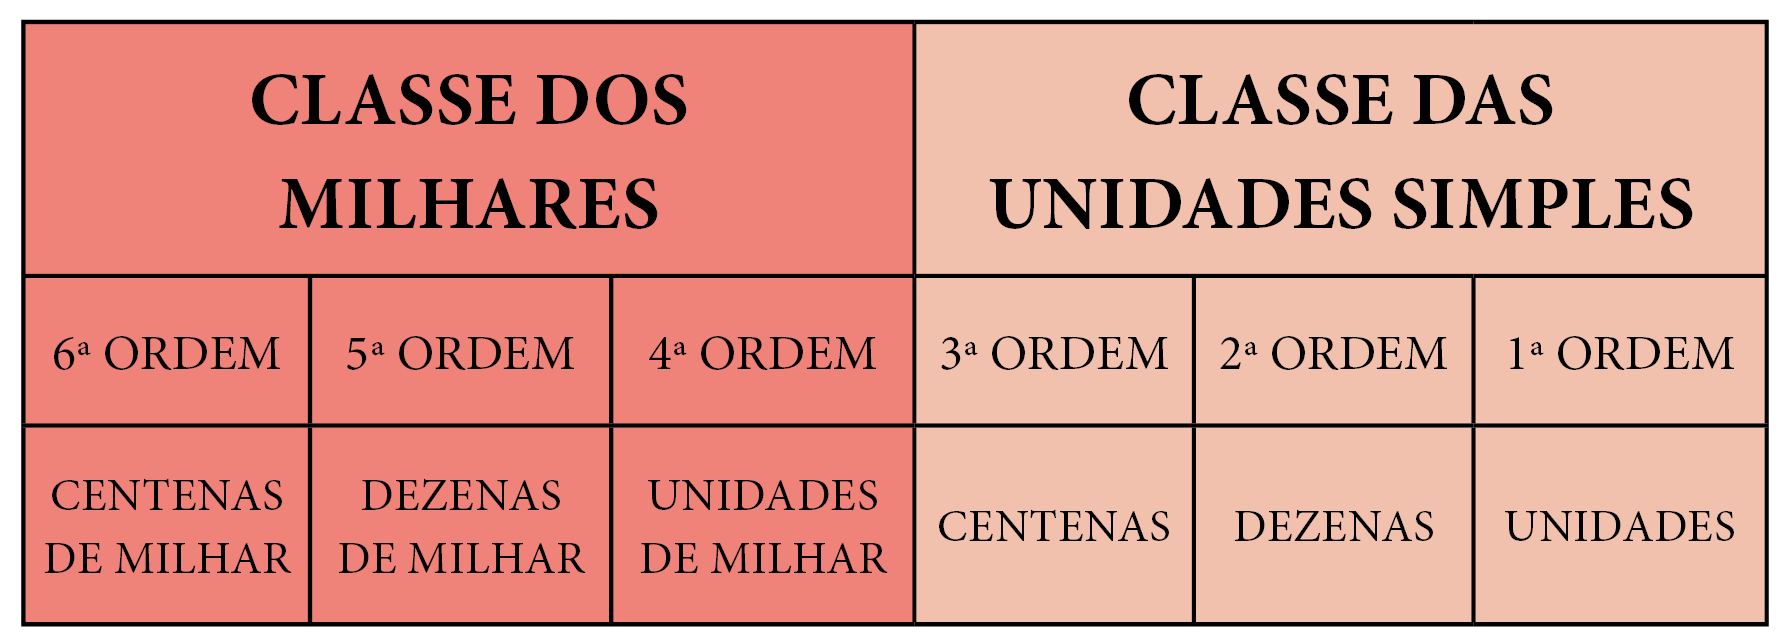
\includegraphics[width=3.55128in,height=1.66618in]{media/image1.png}

Valor posicional ou relativo: é o valor que o algarismo assume
dependendo da classe e da ordem em que ele está posicionado no número.

Exemplo: No número 352.146, o algarismo 5 possui valor posicional ou
relativo igual a 50.000, pois ocupa a 5º ordem, a qual está dentro da
classe dos milhares; ou seja, está na posição da dezena de milhar. Sendo
assim, 5 x 10.000 = 50.000.

Decomposição numérica de acordo com a posição do algarismo:

Exemplo: 389 = 3 x 100 + 8 x 10 + 9}

\colorsec{Atividades}

\num{1} Vilma encontrou um pedaço de papel em sua bolsa com um número escrito:

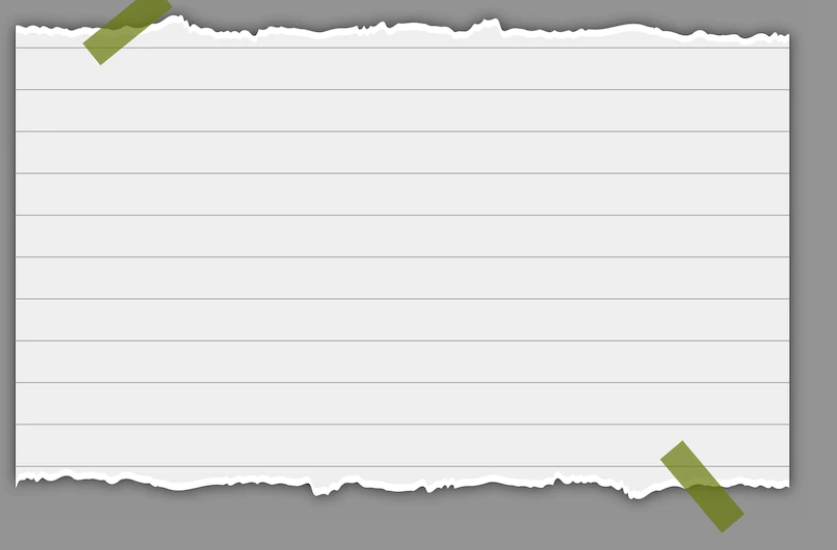
\includegraphics[width=3.30833in,height=2.17391in]{media/image2.png}

%\url{https://img.freepik.com/vetores-gratis/vetor-de-fundo-de-design-de-pedaco-de-papel-rasgado_1055-13108.jpg?w=900\&t=st=1677434705~exp=1677435305~hmac=787f679840c02b57af4cb87ef851030bb83880366602641e4486462d6d3553f8}

%Escrever o número 46 em um pedaço de papel, produzindo assim, a imagem.

\begin{escolha}
\item
  Escreva por extenso como se lê esse número.

\reduline{Quarenta e seis\hfill}

\item
  Se for necessário dividir esse número em grupos de 10, quantos grupos conseguiríamos formar?

\reduline{Conseguiríamos dividir em 4 grupos com 10 unidades e sobrariam 6 unidades. 4 x 10 + 6.\hfill}
\end{escolha}

\num{2} Arnaldo estava contando suas figurinhas e, para isso, montou 8 grupos com
10 figurinhas mais 4 figurinhas em cada um deles.

\begin{escolha}
\item
  Quantas figurinhas Arnaldo possui?

\reduline{8 x 10 + 4 = 84.\hfill}
\linhas{3}

\item
  Como se escreve a quantidade de figurinhas que ele tem por extenso?

\reduline{Oitenta e quatro.\hfill}
\end{escolha}

\num{3} Treine sua criatividade escrevendo:

\begin{escolha}
\item Um número formado por três algarismos iguais.

\reduline{Resposta pessoal. Exemplo: 222.\hfill}

\item Um número formado por três algarismos no qual o 0 (zero) seja o terceiro algarismo.

\reduline{Resposta pessoal. Exemplo: 390.\hfill}

\item Um número formado por três algarismos diferentes.

\reduline{Resposta pessoal. Exemplo: 159.\hfill}

\item Um número com mais de três algarismos.

\reduline{Resposta pessoal. Exemplo: 1.477.\hfill}

\item Mostre os números que você criou para um colega e veja os que ele criou também.
\end{escolha}

\num{4} Escreva os números escritos em cada item e, depois, decomponha esse número conforme o exemplo.

\begin{quote}
Cento e vinte e sete.

127 = 100 + 20 + 7
\end{quote}


\begin{escolha}
\item Trezentos e cinquenta e quatro.

\reduline{300 + 50 + 4\hfill}

\item Duzentos e vinte e oito.

\reduline{200 + 20 + 8\hfill}

\item Quatrocentos e setenta e seis.

\reduline{400 + 70 + 6\hfill}
\end{escolha}

\num{5} Complete a tabela seguindo as instruções.

\begin{longtable}[]{@{}lll@{}}
\toprule
Número escrito por extenso & Número escrito com algarismos & Número
decomposto\tabularnewline
\midrule
\endhead
Quinhentos e vinte e seis & &\tabularnewline
& 435 &\tabularnewline
& & 800 + 30 + 2\tabularnewline
& & 700 + 20 + 9\tabularnewline
\bottomrule
\end{longtable}

\coment{Quinhentos e vinte e seis: 526 = 500 + 20 + 6

Quatrocentos e trinta e cinco: 435 = 400 + 30 + 5

Oitocentos e trinta e dois: 832 = 800 + 30 + 2

Setecentos e vinte e nove: 729 = 700 + 20 + 9}

\num{6} Gabriel, durante sua aula, estava aprendendo a montar números utilizando o
material dourado e montou o seguinte número:

%Produzir uma imagem semelhante a essa abaixo com 5 barras de 10 cubinhos cada e 9 cubinhos separados. Deixar a figura melhor apresentável e, se possível, numa cor parecida com o dourado.

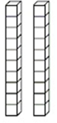
\includegraphics[width=0.47504in,height=1.02509in]{media/image3.png}
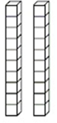
\includegraphics[width=0.47504in,height=1.02509in]{media/image3.png}
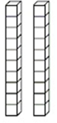
\includegraphics[width=0.47504in,height=1.02509in]{media/image3.png}
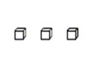
\includegraphics[width=0.75006in,height=0.55838in]{media/image4.png}
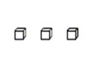
\includegraphics[width=0.75006in,height=0.55838in]{media/image4.png}
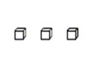
\includegraphics[width=0.75006in,height=0.55838in]{media/image4.png}

Qual é o número representado pelo material dourado na figura?

\reduline{Temos 6 dezenas e 9 unidades, portanto: 6 x 10 + 9 = 69\hfill}
\linhas{1}

\num{7} Complete os quadros abaixo com os número que indicam as quantidades e, em
seguida, escreva por extenso o número encontrado.

\begin{escolha}

\item
  Fernando tem 4 dezenas de lápis mais 2 unidades.

\begin{longtable}[]{@{}ll@{}}
\toprule
Dezena & Unidade\tabularnewline
\midrule
\endhead
&\tabularnewline
\bottomrule
\end{longtable}

Total de lápis que Fernando possui:

\reduline{4 x 10 + 2 = 42. Quarenta e dois lápis.\hfill}

\item Thiago tem 8 dezenas de bolinhas de gude mais 5 unidades.

\begin{longtable}[]{@{}ll@{}}
\toprule
Dezena & Unidade\tabularnewline
\midrule
\endhead
&\tabularnewline
\bottomrule
\end{longtable}

Total de bolinhas de gude que Thiago possui:

\reduline{8 x 10 + 5 = 85. Oitenta e cinco bolinhas de gude.\hfill}
\end{escolha}

\num{8} Realize a decomposição dos números indicados em cada item.

\begin{escolha}
\item 56: \reduline{5 x 10 + 6 = 56\hfill}

\item 73: \reduline{7 x 10 + 3 = 73\hfill}

\item 94: \reduline{9 x 10 + 4 = 94\hfill}

\item 14: \reduline{1 x 10 + 4 = 14\hfill}

\item 81: \reduline{8 x 10 + 1 = 81\hfill}

\item 158: \reduline{1 x 100 + 5 x 10 + 8 = 158\hfill}

\item 649: \reduline{6 x 100 + 4 x 10 + 9\hfill}

\item 784: \reduline{7 x 100 + 8 x 10 + 4\hfill}
\end{escolha}

\num{9} Richard encontrou as seguintes peças de um material dourado:

%Produzir uma imagem semelhante a abaixo mantendo as quantidades pois são importantes para a resolução.

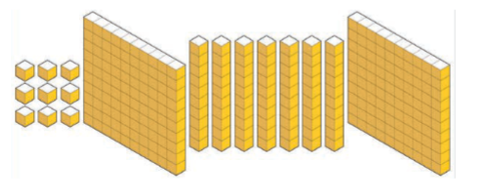
\includegraphics[width=4.02535in,height=1.55013in]{media/image5.png}

Utilizando todas as peças, qual o maior número que Richard conseguirá
representar? Após encontrar o número, escreva-o por extenso.

\reduline{2 x 100 + 7 x 10 + 9 = 279 (Duzentos e setenta e nove)\hfill}
\linhas{2}

\num{10} Monte os números compostos e registre-os nos locais correspondentes.

\begin{escolha}
\item 5 centenas e 4 unidades:

\reduline{504\hfill}

\item 7 dezenas e 2 unidades:

\reduline{72\hfill}

\item 9 centenas, 5 dezenas e 6 unidades:

\reduline{956\hfill}

\item 2 centenas, 6 dezenas e 3 unidades:

\reduline{263\hfill}

\end{escolha}

\num{11} Ligue os retângulos da coluna 1 a um corresponde da coluna 2 que
represente a escrita por extenso do número indicado na primeira coluna.

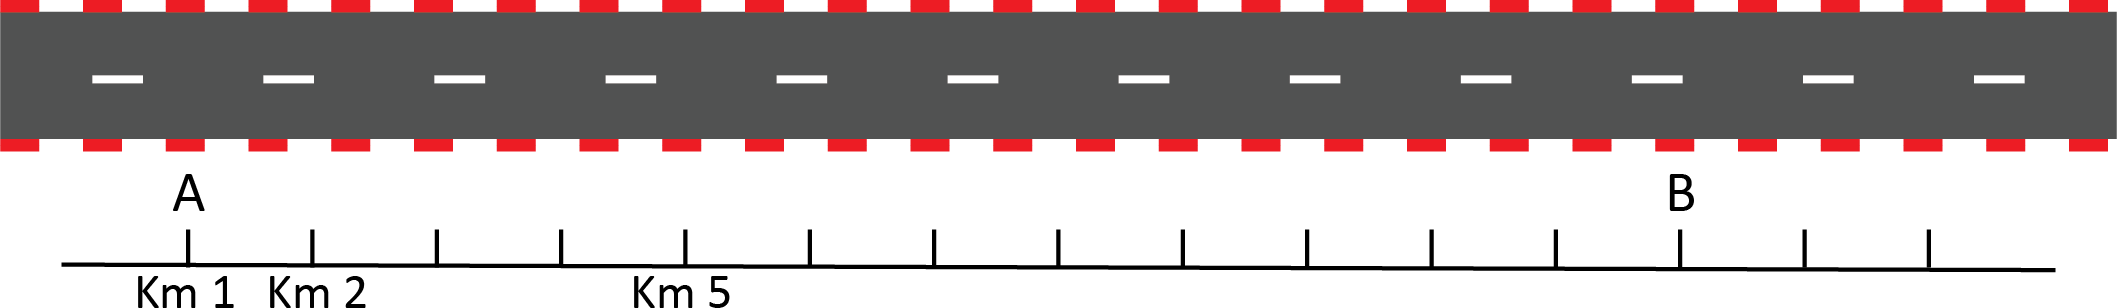
\includegraphics[width=3.85033in,height=1.64181in]{media/image6.png}

%Produzir uma figura conforme a indicada acima: (não colocar os pontos em vermelho que aparecem na figura acima). Não precisa ser colorido. Pose ser feito no padrão e cores do projeto.

\coment{88 deve estar ligado ao oitenta e oito.

283 deve estar ligado ao duzentos e oitenta e três.

57 deve estar ligado a ciquenta e sete.

316 deve estar ligado ao trezentos e dezesseis.}

\num{12} Felipe quer realizar uma corrida e resolveu planejá-la. Para isso, fez
uma linha reta e nela marcou intervalos de 1 km, conforme representado na imagem.

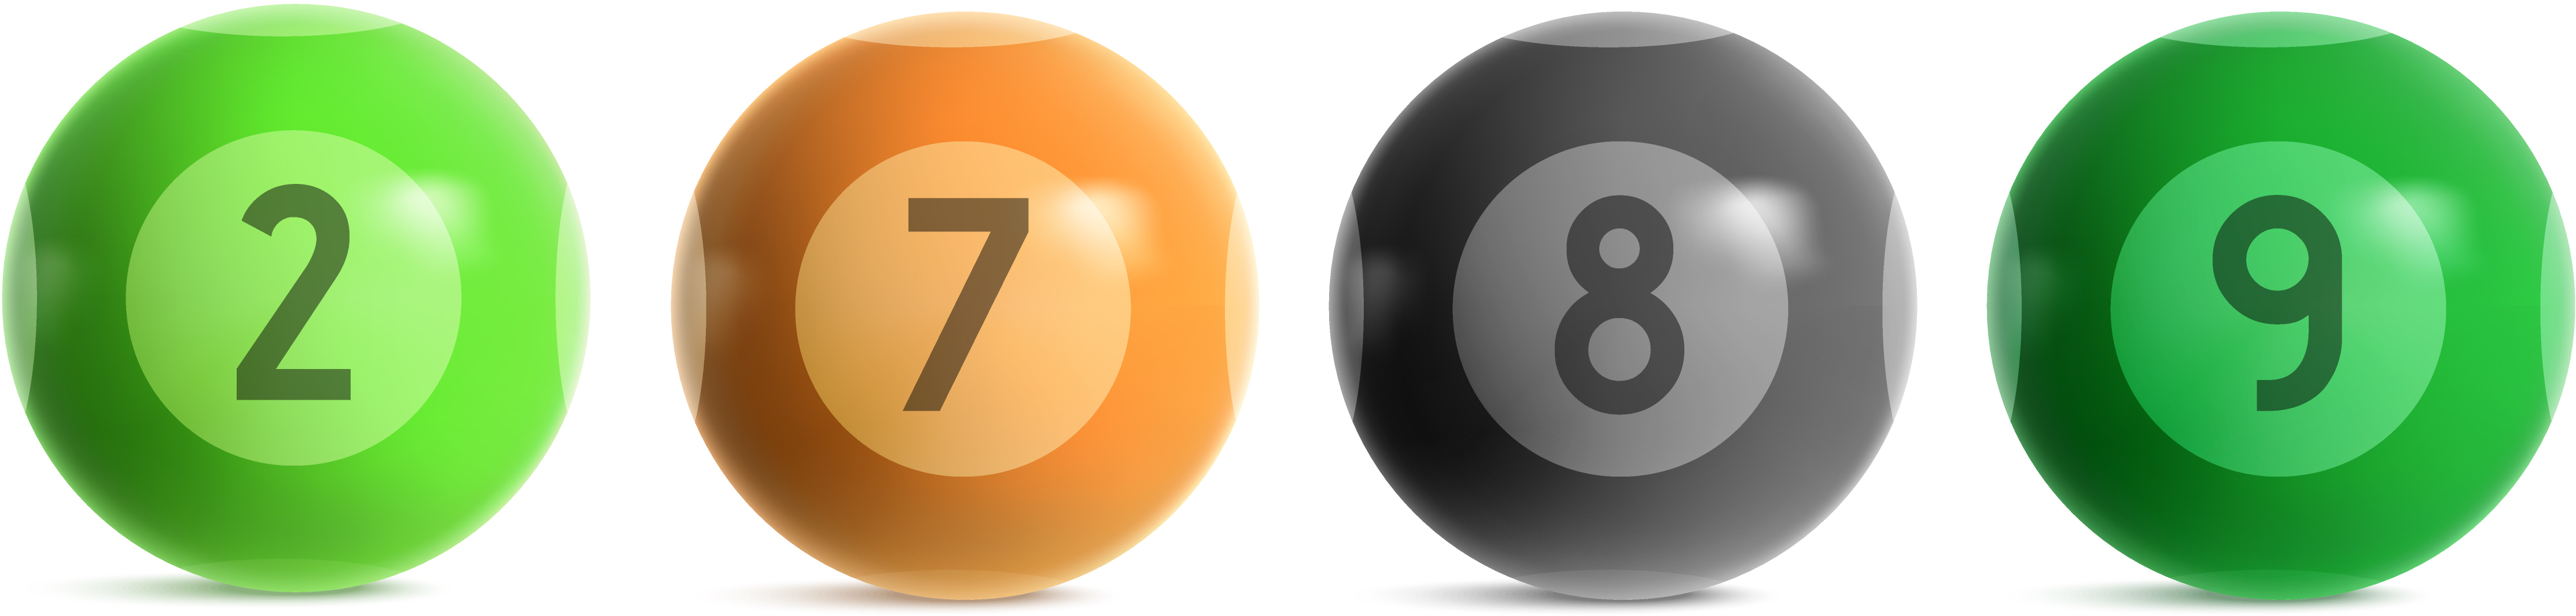
\includegraphics[width=5.90556in,height=0.79514in]{media/image7.png}

%Colocar B no lugar do X no desenho pedido.

%Colocar um desenho de uma pista de corrida com as marcações da forma que estão apresentadas acima. O ponto A deve estar no km 0 e o número de marcações até o ponto B não pode ser alterado.

Ele pretende começar no ponto A e terminar no ponto B. Se Felipe
conseguiu completar a corrida, ele parou na marcação

\begin{minipage}{.5\textwidth}
\begin{escolha}
\item Km 9.

\item Km 10.

\item Km 11.

\item Km 12.
\end{escolha}
\end{minipage}
\sidetext{Como ele saiu do ponto A, que está em cima da marcação km 0, e chegou ao
ponto B, que está a 12 marcações de distância do ponto, podemos concluir
que ele parou no km 12; ou seja, percorreu 12 km.

Explore ao máximo com os alunos a colocação dos números na reta numérica,
já que é um conceito essencial em outros assuntos.}

\num{13} A bolas representadas fazem parte de um jogo conhecido como
bilhar ou sinuca.

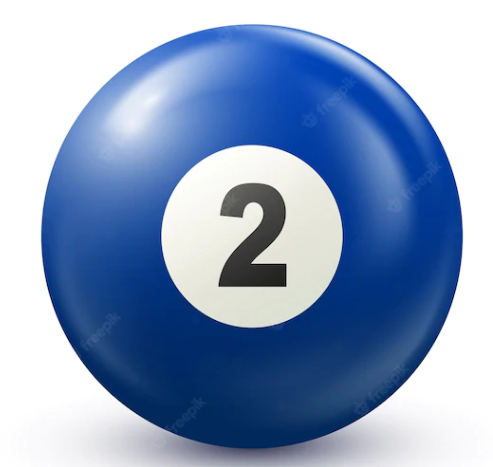
\includegraphics[width=1.40833in,height=1.33406in]{media/image8.png}

%\url{https://img.freepik.com/vetores-premium/bola-de-bilhar-azul-com-numero-2-snooker-ou-bola-de-loteria-em-fundo-branco-ilustracao_390775-925.jpg?w=740}

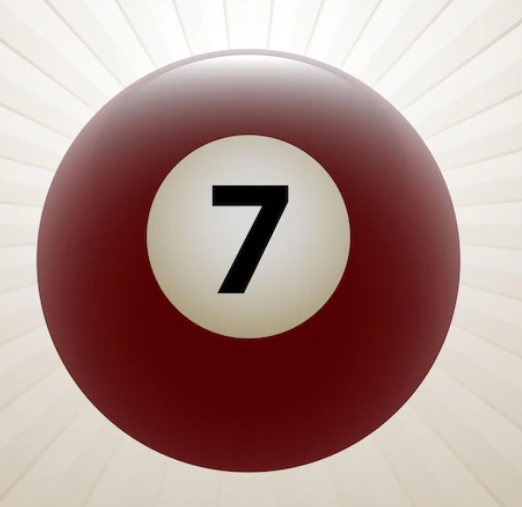
\includegraphics[width=1.66667in,height=1.61877in]{media/image9.png}

%\url{https://img.freepik.com/vetores-premium/bilhar_672017-1383.jpg?w=740}

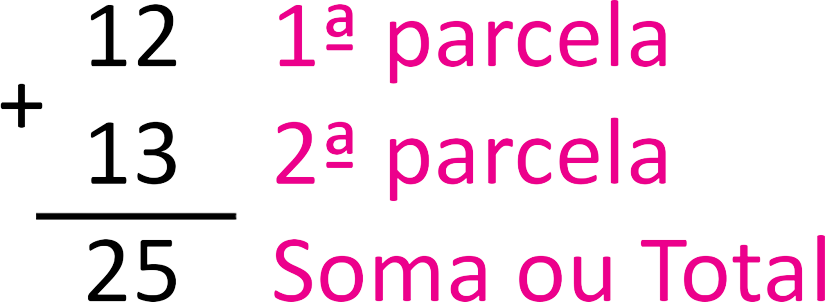
\includegraphics[width=1.68333in,height=1.36449in]{media/image10.png}

%\url{https://img.freepik.com/psd-premium/ilustracao-3d-da-bola-de-bilhar-oito_446709-517.jpg?w=740}

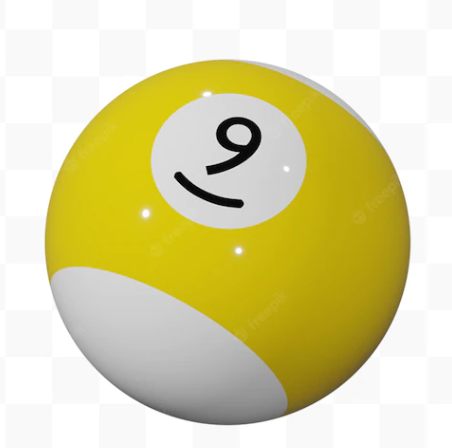
\includegraphics[width=1.61667in,height=1.60236in]{media/image11.png}

%\url{https://img.freepik.com/psd-premium/bola-de-bilhar-3d-numero-9_592419-130.jpg?w=740}

%Colocar as bolinhas na mesma linha

Observando os números representados em cada bola, responda:

\begin{escolha}
\item Qual o maior número?

\reduline{9 (nove)\hfill}

\item Qual o menor número com 3 exatamente ordens que podemos formar?

\reduline{278 (duzentos e setenta e oito)\hfill}

\item Qual o maior número par que podemos formar?

\reduline{9.872 (nove mil oitocentos e setenta e dois)\hfill}

\end{escolha}

\coment{Explore mais exemplos com os alunos para estimular a criatividade
e a formação de números.}

\colorsec{Treino}

\num{1} Amanda estava brincando no escritório de seu pai quando
encontrou um pedaço de papel com uma anotação.

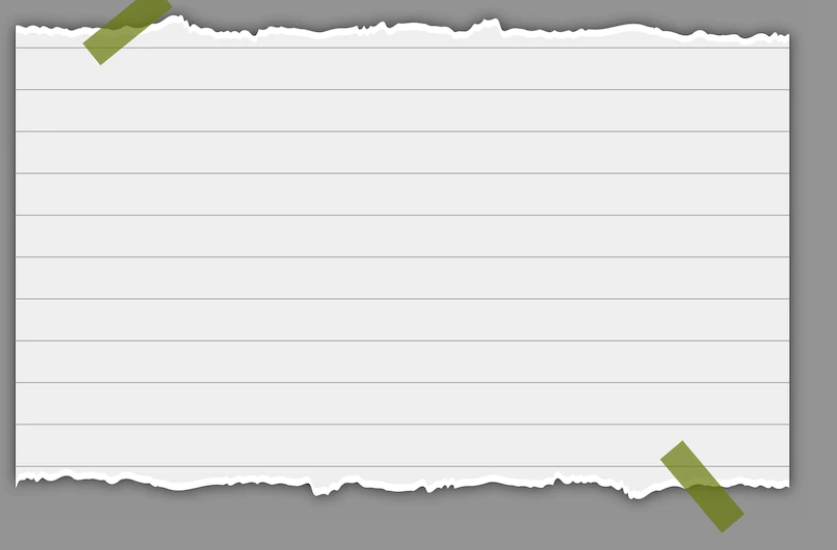
\includegraphics[width=3.30833in,height=2.17391in]{media/image2.png}

%\url{https://img.freepik.com/vetores-gratis/vetor-de-fundo-de-design-de-pedaco-de-papel-rasgado_1055-13108.jpg?w=900\&t=st=1677434705~exp=1677435305~hmac=787f679840c02b57af4cb87ef851030bb83880366602641e4486462d6d3553f8}

%Um pedaço de papel com a frase abaixo escrita

Faturamento diário: 734 reais

Lembrando das aulas de matemática, ela resolveu decompor o número escrito
no papel. Qual a decomposição correta que Amanda deverá fazer desse
número?

\begin{minipage}{.5\textwidth}
\begin{escolha}
\item
  700 + 30 + 4
\item
  70 + 3 + 4
\item
  700 + 40 + 3
\item
  70 + 300 + 4
\end{escolha}
\end{minipage}
\sidetext{SAEB: Compor ou decompor números naturais de até 6 ordens na forma aditiva, ou em suas ordens, ou em adições e multiplicações.
BNCC: EF03MA04 -- Estabelecer a relação entre números naturais e pontos da reta numérica para
utilizá-la na ordenação dos números naturais e também na construção de fatos da adição e da
subtração, relacionando-os com deslocamentos para a direita ou para a esquerda.}

\num{2} Na reta numérica a seguir, o ponto P representa o número 540 e o ponto U representa o número 590.

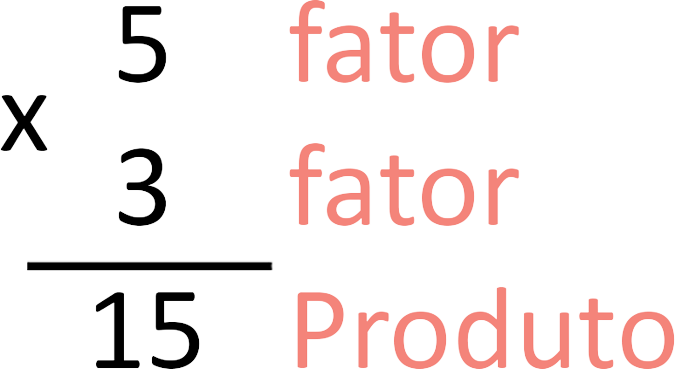
\includegraphics[width=3.03205in,height=0.81228in]{media/image12.png}

%Na figura acima ao invés de 960 favor colocar 540 e no lugar de 1 010 colocar 590.

Em qual ponto temos a representação do número 570, sabendo-se que a
distância entre dois pontos consecutivos é de 10 unidades?

\begin{minipage}{.5\textwidth}
\begin{escolha}

\item
  Q
\item
  R
\item
  S
\item
  T
\end{escolha}
\end{minipage}
\sidetext{SAEB: Identificar a ordem ocupada por um algarismo ou seu valor posicional (ou valor relativo) em um número natural de até 6 ordens.
BNCC: EF03MA01 -- Ler, escrever e comparar números naturais de até a ordem de unidade de milhar, estabelecendo relações entre os registros numéricos e em língua materna.}

\num{3} Utilizando o material dourado, Ana Letícia montou a seguinte número:

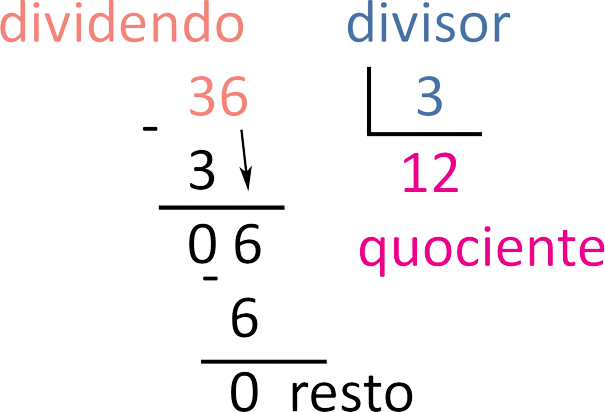
\includegraphics[width=4.13369in,height=0.83341in]{media/image13.png}

%Construir uma figura dessa forma mantendo a quantidade de 5 placas (10 cubinhos x10 cubinhos) e 9 cubinhos pequenos.

Qual o número representado por Ana Letícia?

\begin{minipage}{.5\textwidth}
\begin{escolha}
\item
  59
\item
  159
\item
  509
\item
  1.509
\end{escolha}
\end{minipage}
\sidetext{SAEB: Compor ou decompor números naturais de até 6 ordens na forma aditiva, ou em suas ordens, ou em adições e multiplicações.
BNCC: EF03MA01 -- Ler, escrever e comparar números naturais de até a ordem de unidade de milhar, estabelecendo relações entre os registros numéricos e em língua materna.}

\chapter{Cálculos}
\markboth{Módulo 2}{}

\colorsec{Habilidades do SAEB}

\begin{itemize}
\item Calcular o resultado de adições ou subtrações envolvendo números
naturais de até 6 ordens.

\item Calcular o resultado de multiplicações ou divisões envolvendo números
naturais de até 6 ordens.

\item Associar o quociente de uma divisão com resto zero de um número
natural de até 6 ordens por 2, 3, 4, 5 e 10 às ideias de metade, terça,
quarta, quinta e décima parte.

\item Resolver problemas de adição ou de subtração, envolvendo números
naturais de até 6 ordens, com os significados de juntar, acrescentar,
separar, retirar, comparar ou completar.

\item Resolver problemas de multiplicação ou de divisão, envolvendo números
naturais de até 6 ordens, com os significados de formação de grupos
iguais (incluindo repartição equitativa e medida), proporcionalidade ou
disposição retangular.
\end{itemize}

\coment{Habilidades da BNCC: EF03MA06, EF03MA07, EF03MA08.}

\conteudo{
Assim como todos os conteúdos que envolvem as quatro operações básicas, este módulo é essencial e seu estudo deve ser feito com tempo para bastante treino. Relembre com os alunos cada detalhe
e os algoritmos de adição, subtração, multiplicação e divisão, dando 
ênfase à divisão, que geralmente é o maior desafio enfrentado pelos alunos.

Adição:

%Fazer a imagem abaixo segundo os padrões do projeto.

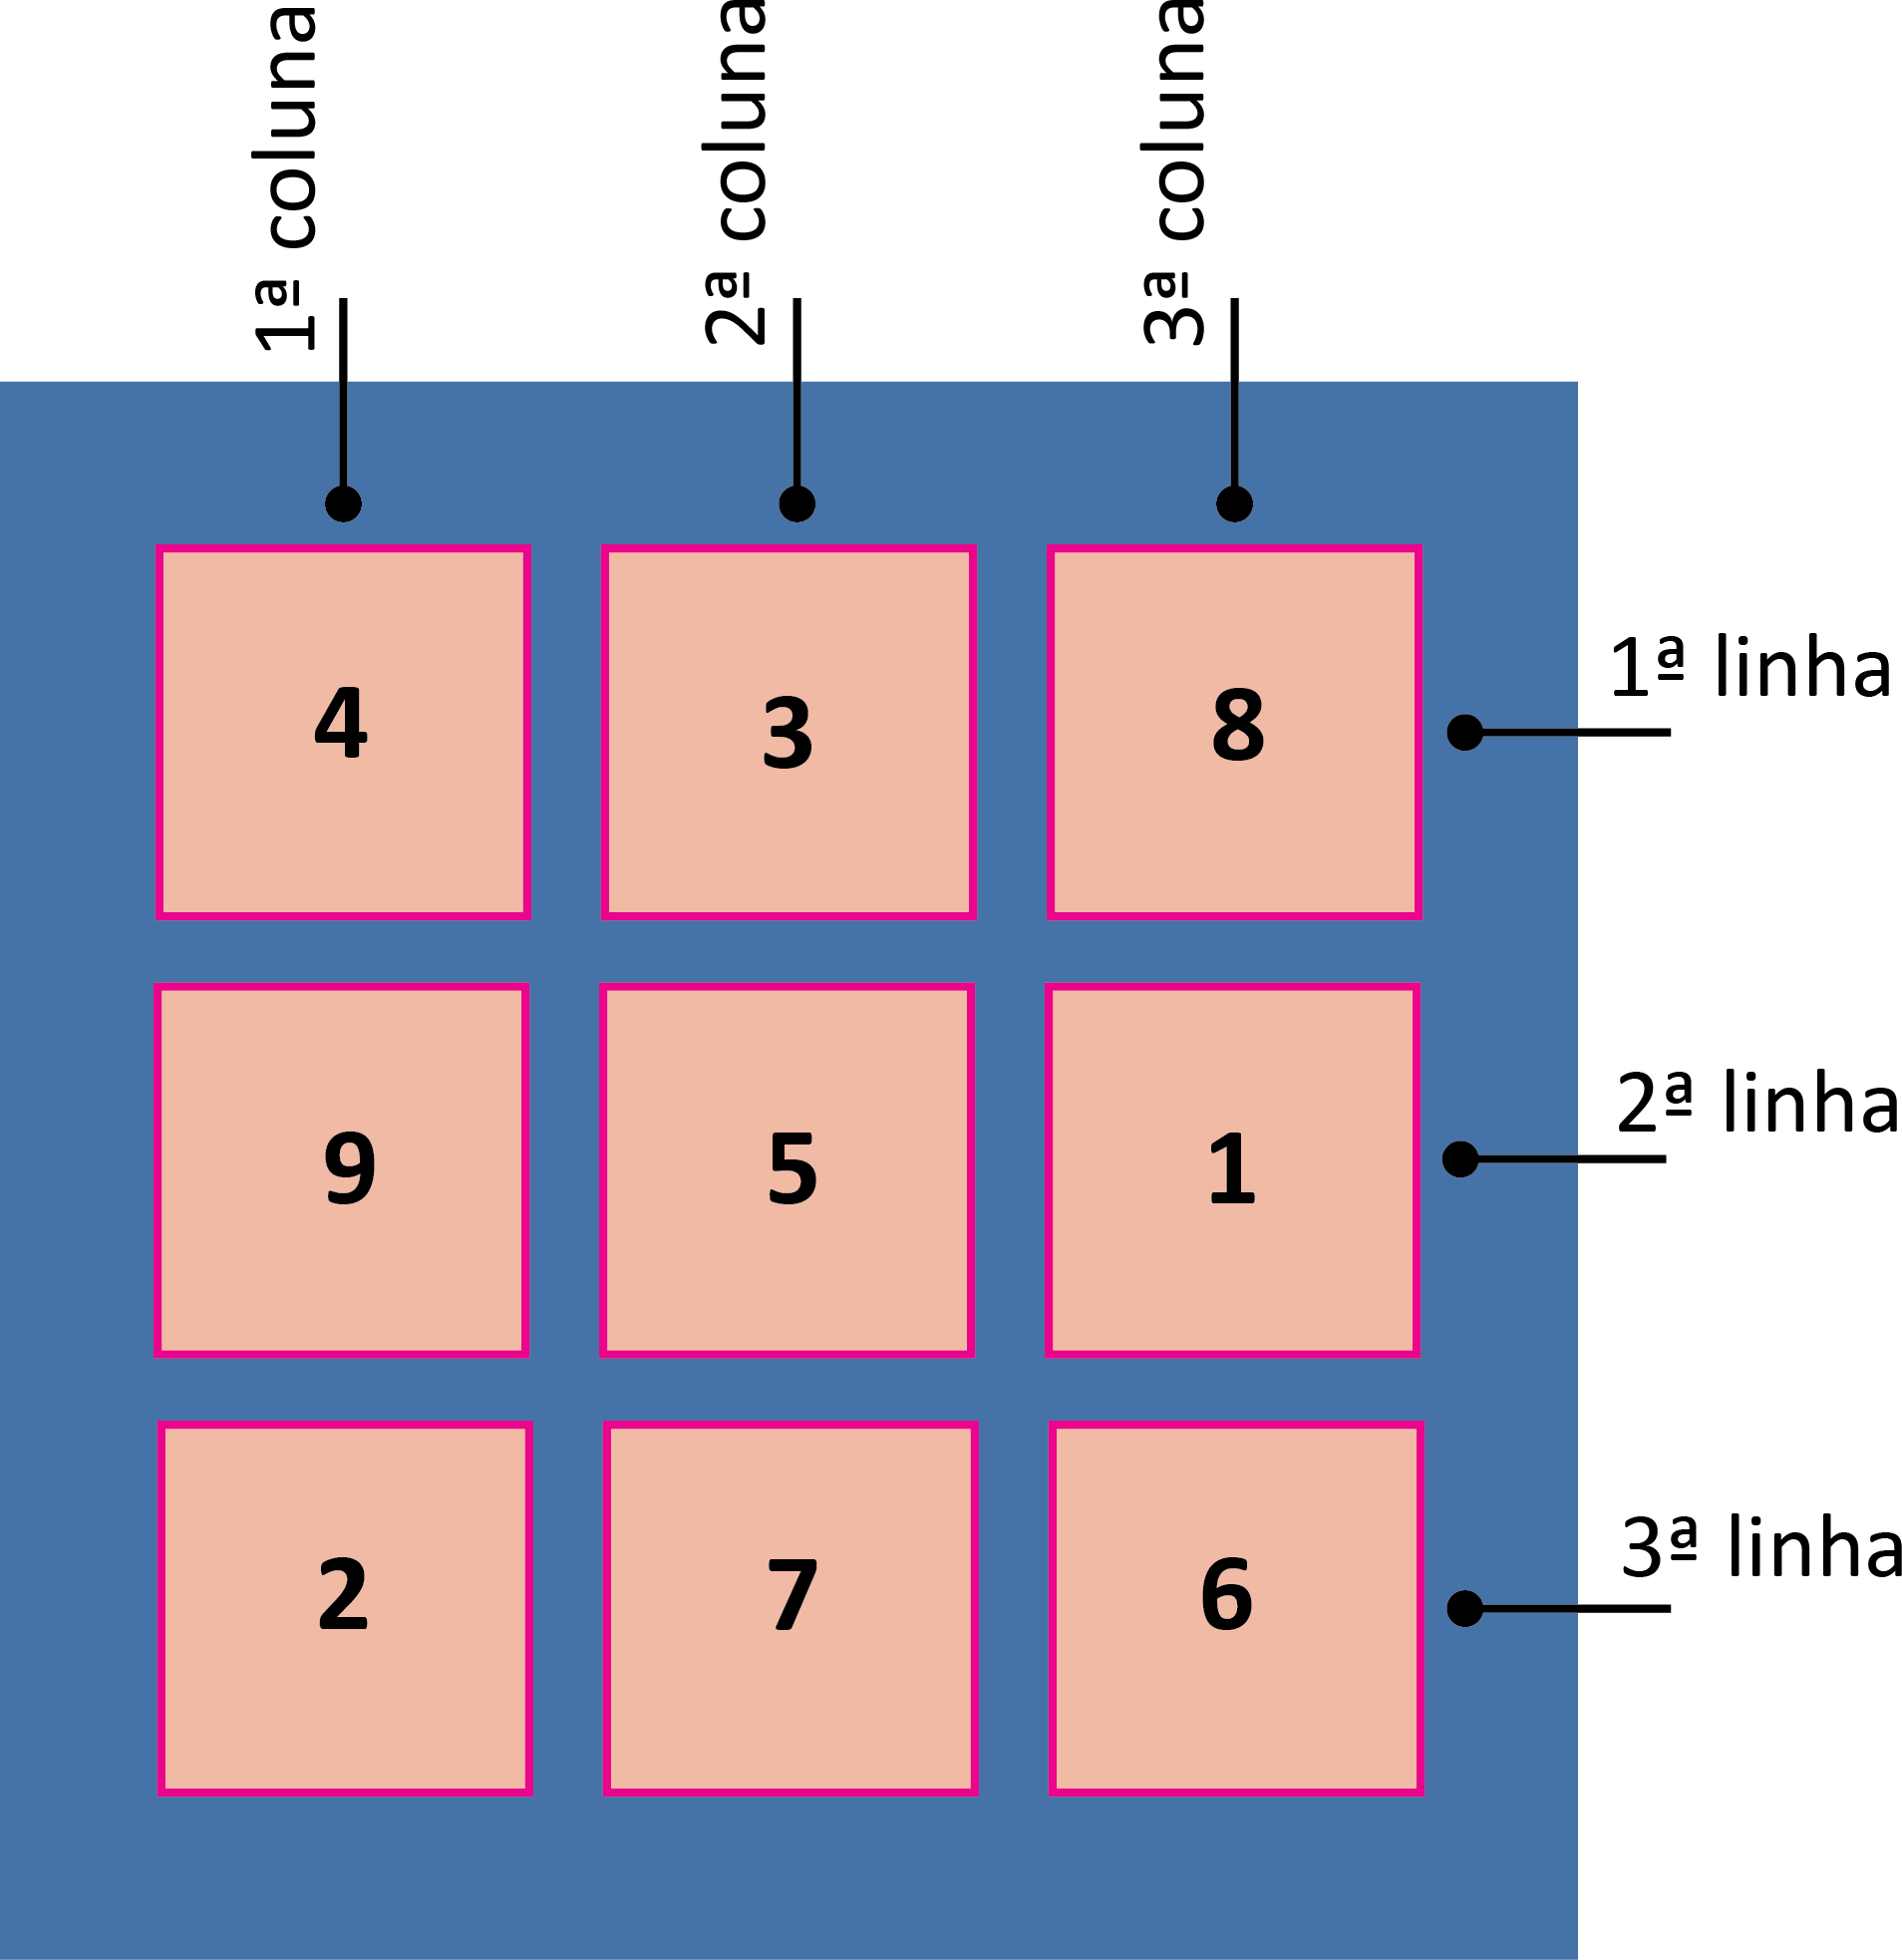
\includegraphics[width=2.26282in,height=1.19473in]{media/image14.png}

Subtração:

%Fazer a imagem abaixo segundo os padrões do projeto.

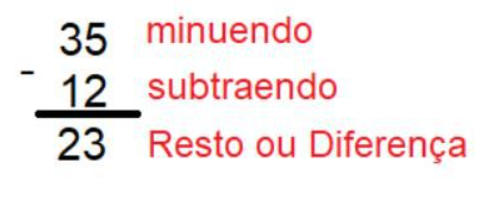
\includegraphics[width=2.55128in,height=1.04961in]{media/image15.png}

Multiplicação:

%Fazer a imagem abaixo segundo os padrões do projeto.

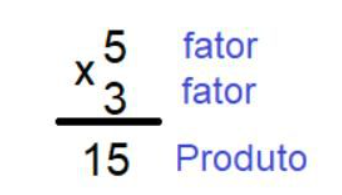
\includegraphics[width=1.92308in,height=1.09649in]{media/image16.png}

Divisão:

%Fazer a imagem abaixo segundo os padrões do projeto.

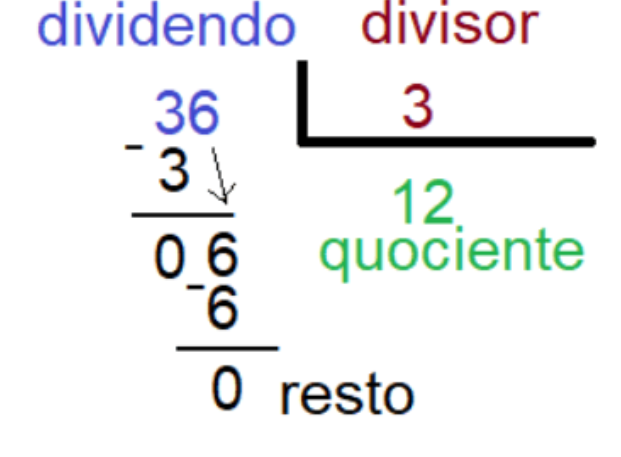
\includegraphics[width=2.26923in,height=1.66995in]{media/image17.png}
}

\colorsec{Atividades}

\num{1} Assinale o que deve ser feito em cada item para que ocorra o que se pede.

\begin{escolha}

\item
  Transformar 262 em 362.

\begin{boxlist}
\boxitem[] Adicionar 1.

\boxitem[] Adicionar 10.

\boxitem[]Adicionar 100.
\end{boxlist}

\item
  Transformar 1.100 em 1.000.

\begin{boxlist}
\boxitem[] Subtrair 1.

\boxitem[] Subtrair 10.

\boxitem[]Subtrair 100.
\end{boxlist}

\item
  Transformar 238 em 239.

\begin{boxlist}
\boxitem[] Adicionar 1.

\boxitem[] Subtrair 1.

\boxitem[]Adicionar 10.
\end{boxlist}

\end{escolha}

\num{2} Utilize os sinais \textless{} (menor que), \textgreater{} (maior que) ou
= (igual a) em cada situação para comparar as quantidade representadas.

\begin{escolha}
\item
  7 \reduline{Menor que, \textless{}\hfill} 14
\item
  21 \reduline{Maior que, \textgreater{}\hfill} 5
\item
  1 + 3 \reduline{Igual a, =\hfill} 2 + 2
\item
  5 + 2 \reduline{Maior que, \textgreater{}\hfill} 7 -- 1
\item
  20 -- 1 \reduline{Igual a, =\hfill} 19
\item
  Treze \reduline{Menor que, \textless{}\hfill} quinze
\end{escolha}

\num{3} Ligue cada operação que está na coluna 1 com o seu resultado correto na coluna 2.

%Os números  devem aparecer na coluna da direita.

\begin{multicols}{2}
84 + 12

60 -- 23

67 -- 58

50 -- 2 x (5 + 15) + 2

2 + 8 -- 2 x (1 + 2)

\colunmbreak

37

9

96

4

12
\end{multicols}

%Colocar as operações acima e os resultados de ambas as colunas em retângulos

%Deixar um espaço em branco  para os alunos efetuarem os cálculos necessários

\coment{Explore ao máximo com os alunos o conceito de quais operações
devem ser realizadas primeiro e, assim, ajude na fixação desse conceito.

84 + 12 = 96

60 -- 23 = 37

67 -- 58 = 9

50 -- 2 x (5 + 15) + 2 = 50 -- 40 + 2 = 12

2 + 8 -- 2 x (1 + 2) = 2 + 8 -- 6 = 4}

\num{4} Observe atentamente a figura dada e, em seguida, responda ao que se pede em cada item.

%Produzir uma figura semelhante a abaixo nos moldes do projeto mas os números devem ser os mesmos. 
%Imagino que possa ser feita uma tabela simples.

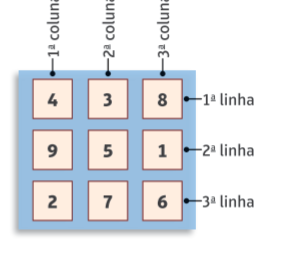
\includegraphics[width=2.37521in,height=2.18352in]{media/image21.png}

\begin{escolha}
\item Qual a soma de todos os números que estão na primeira coluna?

\reduline{4 + 9 + 2 = 15\hfill}
\linhas{2}

\item Qual a soma de todos os números que estão na segunda coluna?

\reduline{3 + 5 + 7 = 15\hfill}
\linhas{2}

\item Qual a soma de todos os números que estão na terceira coluna?

\reduline{8 + 1 + 6 = 15\hfill}
\linhas{2}

\item O que você percebe quando compara os resultados da soma dos números de cada coluna?

\reduline{A soma sempre resulta em 15.\hfill}
\linhas{2}

\item Qual a soma dos números que estão na 1º linha?

\reduline{4 + 3 + 8 = 15\hfill}
\linhas{2}

\item Qual a soma dos números que estão na 2º linha?

\reduline{9 + 5 + 1 = 15\hfill}
\linhas{2}

\item Qual a soma dos números que estão na 3º linha?

\reduline{2 + 7 + 6 = 15\hfill}
\linhas{2}

\item O que você percebe quando compara os resultados da soma dos números de cada linha?

\reduline{A soma sempre resulta em 15.\hfill}
\linhas{2}
\end{escolha}

\num{5} Vicente vendeu, em um evento que ocorreu na praça central de uma pequena
cidade do interior do Brasil, 6 sorvetes de chocolate, 8 de morango, 3
de groselha e 5 de creme. Quantas unidades de sorvete Vicente vendeu durante esse evento?

\reduline{6 + 8 + 3 + 5 = 22 unidades de sorvete foram vendidas por Vicente.\hfill}
\linhass{2}

\num{6} A receita de um bolo diz que inicialmente devemos colocar 260 g de
farinha de trigo e misturar com outros ingredientes como ovos, açúcar e
leite. Em seguida, devemos colocar mais 135 g de farinha de trigo para a
massa ficar no ponto ideal. Qual foi a quantidade total de farinha
utilizada nessa receita?

%imagem de freepik disponível no link https://br.freepik.com/fotos-premium/nao-ha-nada-que-eu-ame-mais-do-que-assar-foto-recortada-de-uma-mulher-decorando-um-bolo-em-sua-cozinha_27771468.htm#query=making\%20cake\&position=5\&from_view=search\&track=robertav1_2_sidr

\reduline{260 + 135 = 395 g\hfill}
\linhas{2}

\num{7} Raquel sempre amou confeitaria e, por isso, decidiu começar uma pequena empresa que faz doces para festas. Para o próximo final de semana, ela
recebeu a seguinte encomenda por mensagem de texto em seu celular:

\textbf{Encomenda para a festa da Maria}

\begin{itemize}
\item 275 brigadeiros

\item 165 beijinhos

\item 245 cajuzinhos
\end{itemize}

Calcule o total de unidades de doces que Raquel terá que fazer para entregar essa encomenda.

\reduline{275 + 165 + 245 = 685 unidades de doces.\hfill}
\linhas{3}

\num{8} Complete o quadro, proposto pela professora Marina, transformando
as adições em multiplicações; em seguida, encontre o resultado. Para isso, siga o modelo.

\begin{longtable}[]{@{}lll@{}}
\toprule
Adição de parcelas iguais & Multiplicação & Resultado\tabularnewline
\midrule
\endhead
8 + 8 + 8 & 3 x 8 & 24\tabularnewline
10 + 10 + 10 + 10 + 10 & &\tabularnewline
6 + 6 + 6 + 6 & &\tabularnewline
5 + 5 + 5 + 5 + 5 + 5 + 5 & &\tabularnewline
12 + 12 + 12 + 12 + 12 & &\tabularnewline
\bottomrule
\end{longtable}

\coment{
\begin{longtable}[]{@{}lll@{}}
\toprule
Adição de parcelas iguais & Multiplicação & Resultado\tabularnewline
\midrule
\endhead
8 + 8 + 8 & 3 x 8 & 24\tabularnewline
10 + 10 + 10 + 10 + 10 & 5 x 10 & 50\tabularnewline
6 + 6 + 6 + 6 & 4 x 6 & 24\tabularnewline
5 + 5 + 5 + 5 + 5 + 5 + 5 & 5 x 7 & 35\tabularnewline
12 + 12 + 12 + 12 + 12 & 5 x 12 & 60\tabularnewline
\bottomrule
\end{longtable}
}

\num{9} João possui uma distribuidora de ovos e acabou de receber 15 caixas com 252
ovos cada uma. Para que João venda essa mercadoria, ele faz embalagens
com 12 ovos cada uma. Quantas embalagens João conseguirá fazer para
colocar à venda utilizando os ovos que acabou de receber em sua distribuidora?

%\url{https://img.freepik.com/fotos-gratis/ovos-na-superficie-rosa_58702-1950.jpg?w=1060\&t=st=1677435684~exp=1677436284~hmac=6c6204dcded4c4d80a06169fee49d53df4b2636105a2c7b3dbe5365007ceae9a}

\reduline{(15 x 252):12 = 315 embalagens com 12 ovos cada uma.\hfill}

\reduline{É sempre recomendado escrever a expressão formada pela interpretação do enunciado, pois assim os alunos vão aprendendo a transformar textos em linguagem
matemática.\hfill}

\num{10} Brenda se deparou com uma divisão em sua prova de matemática. Para esse
cálculo, aparecia o número 5.192 como dividendo e o número 22 como divisor. Sabendo-se que
Brenda acertou essa questão, qual foi o quociente encontrado por ela?

\coment{Explore também divisões com dividendos maiores.}

\reduline{5.192 : 22 = 236\hfill}
\linhas{3}

\num{11} A mãe de Beatriz comprou uma caixa de bombons para presentear seus
quatro filhos. Na caixa, os bombons estavam distribuídos em 8 fileiras
com 9 bombons em cada. Se ela irá dividir a quantidade total de bombons
igualmente entre seus filhos, quantos bombons Beatriz receberá?

\reduline{(8 x 9) : 4 = 18\hfill}

\reduline{Beatriz receberá 18 bombons, assim como seus irmãos.\hfill}
\linhas{2}



\num{12} Observe a conversa entre Rebeca, Raquel e Renata no sítio do avô de Rebeca.

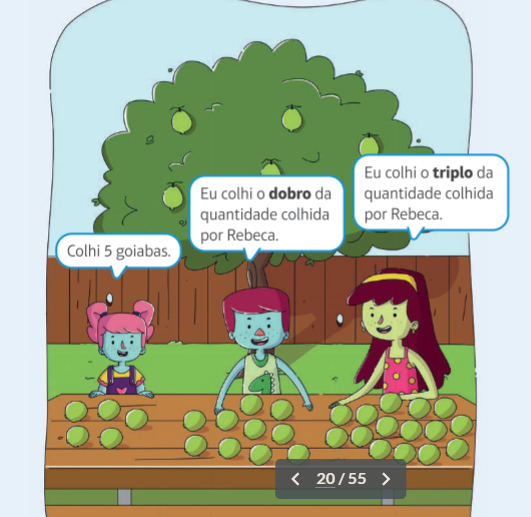
\includegraphics[width=4.42538in,height=4.30871in]{media/image24.png}

%Fazer uma ilustração nos moldes dessa, colocando o nome de cada menina na lateral da mesa a frente delas. Na fala de Renata trocar Rebeca por Raquel. Trocar goiabas por maçãs no texto e nas frutas em cima da mesa. Trocar a palavra dobro na historinha por triplo e aumentar o número de frutas da mesa para 15 na frente dessa menina. Trocar a quantidade frutas na frente da terceira menina para 45.

\begin{escolha}
\item Qual a quantidade de maçãs que Rebeca colheu?

\reduline{5\hfill}
\linhas{2}

\item Qual a quantidade de maçãs que Raquel colheu?

\reduline{3 x 5 = 15\hfill}
\linhas{2}

\item Qual a quantidade de maçãs que Renata colheu?

\reduline{3 x 15 = 45\hfill}
\linhas{2}
\end{escolha}

\num{13} Complete cada frase com a palavra dobro ou com a palavra triplo.

\begin{escolha}
\item
  O \reduline{dobro\hfill} de 10 é 20.
\item
  O \reduline{triplo\hfill} de 6 é 18.
\item
  O \reduline{dobro\hfill} de 7 é 14.
\item
  O \reduline{triplo\hfill} de 8 é 24.
\end{escolha}

\num{14} No quadro branco da professora Adriana foram escritos os seguintes números:

%Construir uma figura conforme a abaixo. Os números importam e devem ser os mesmos.

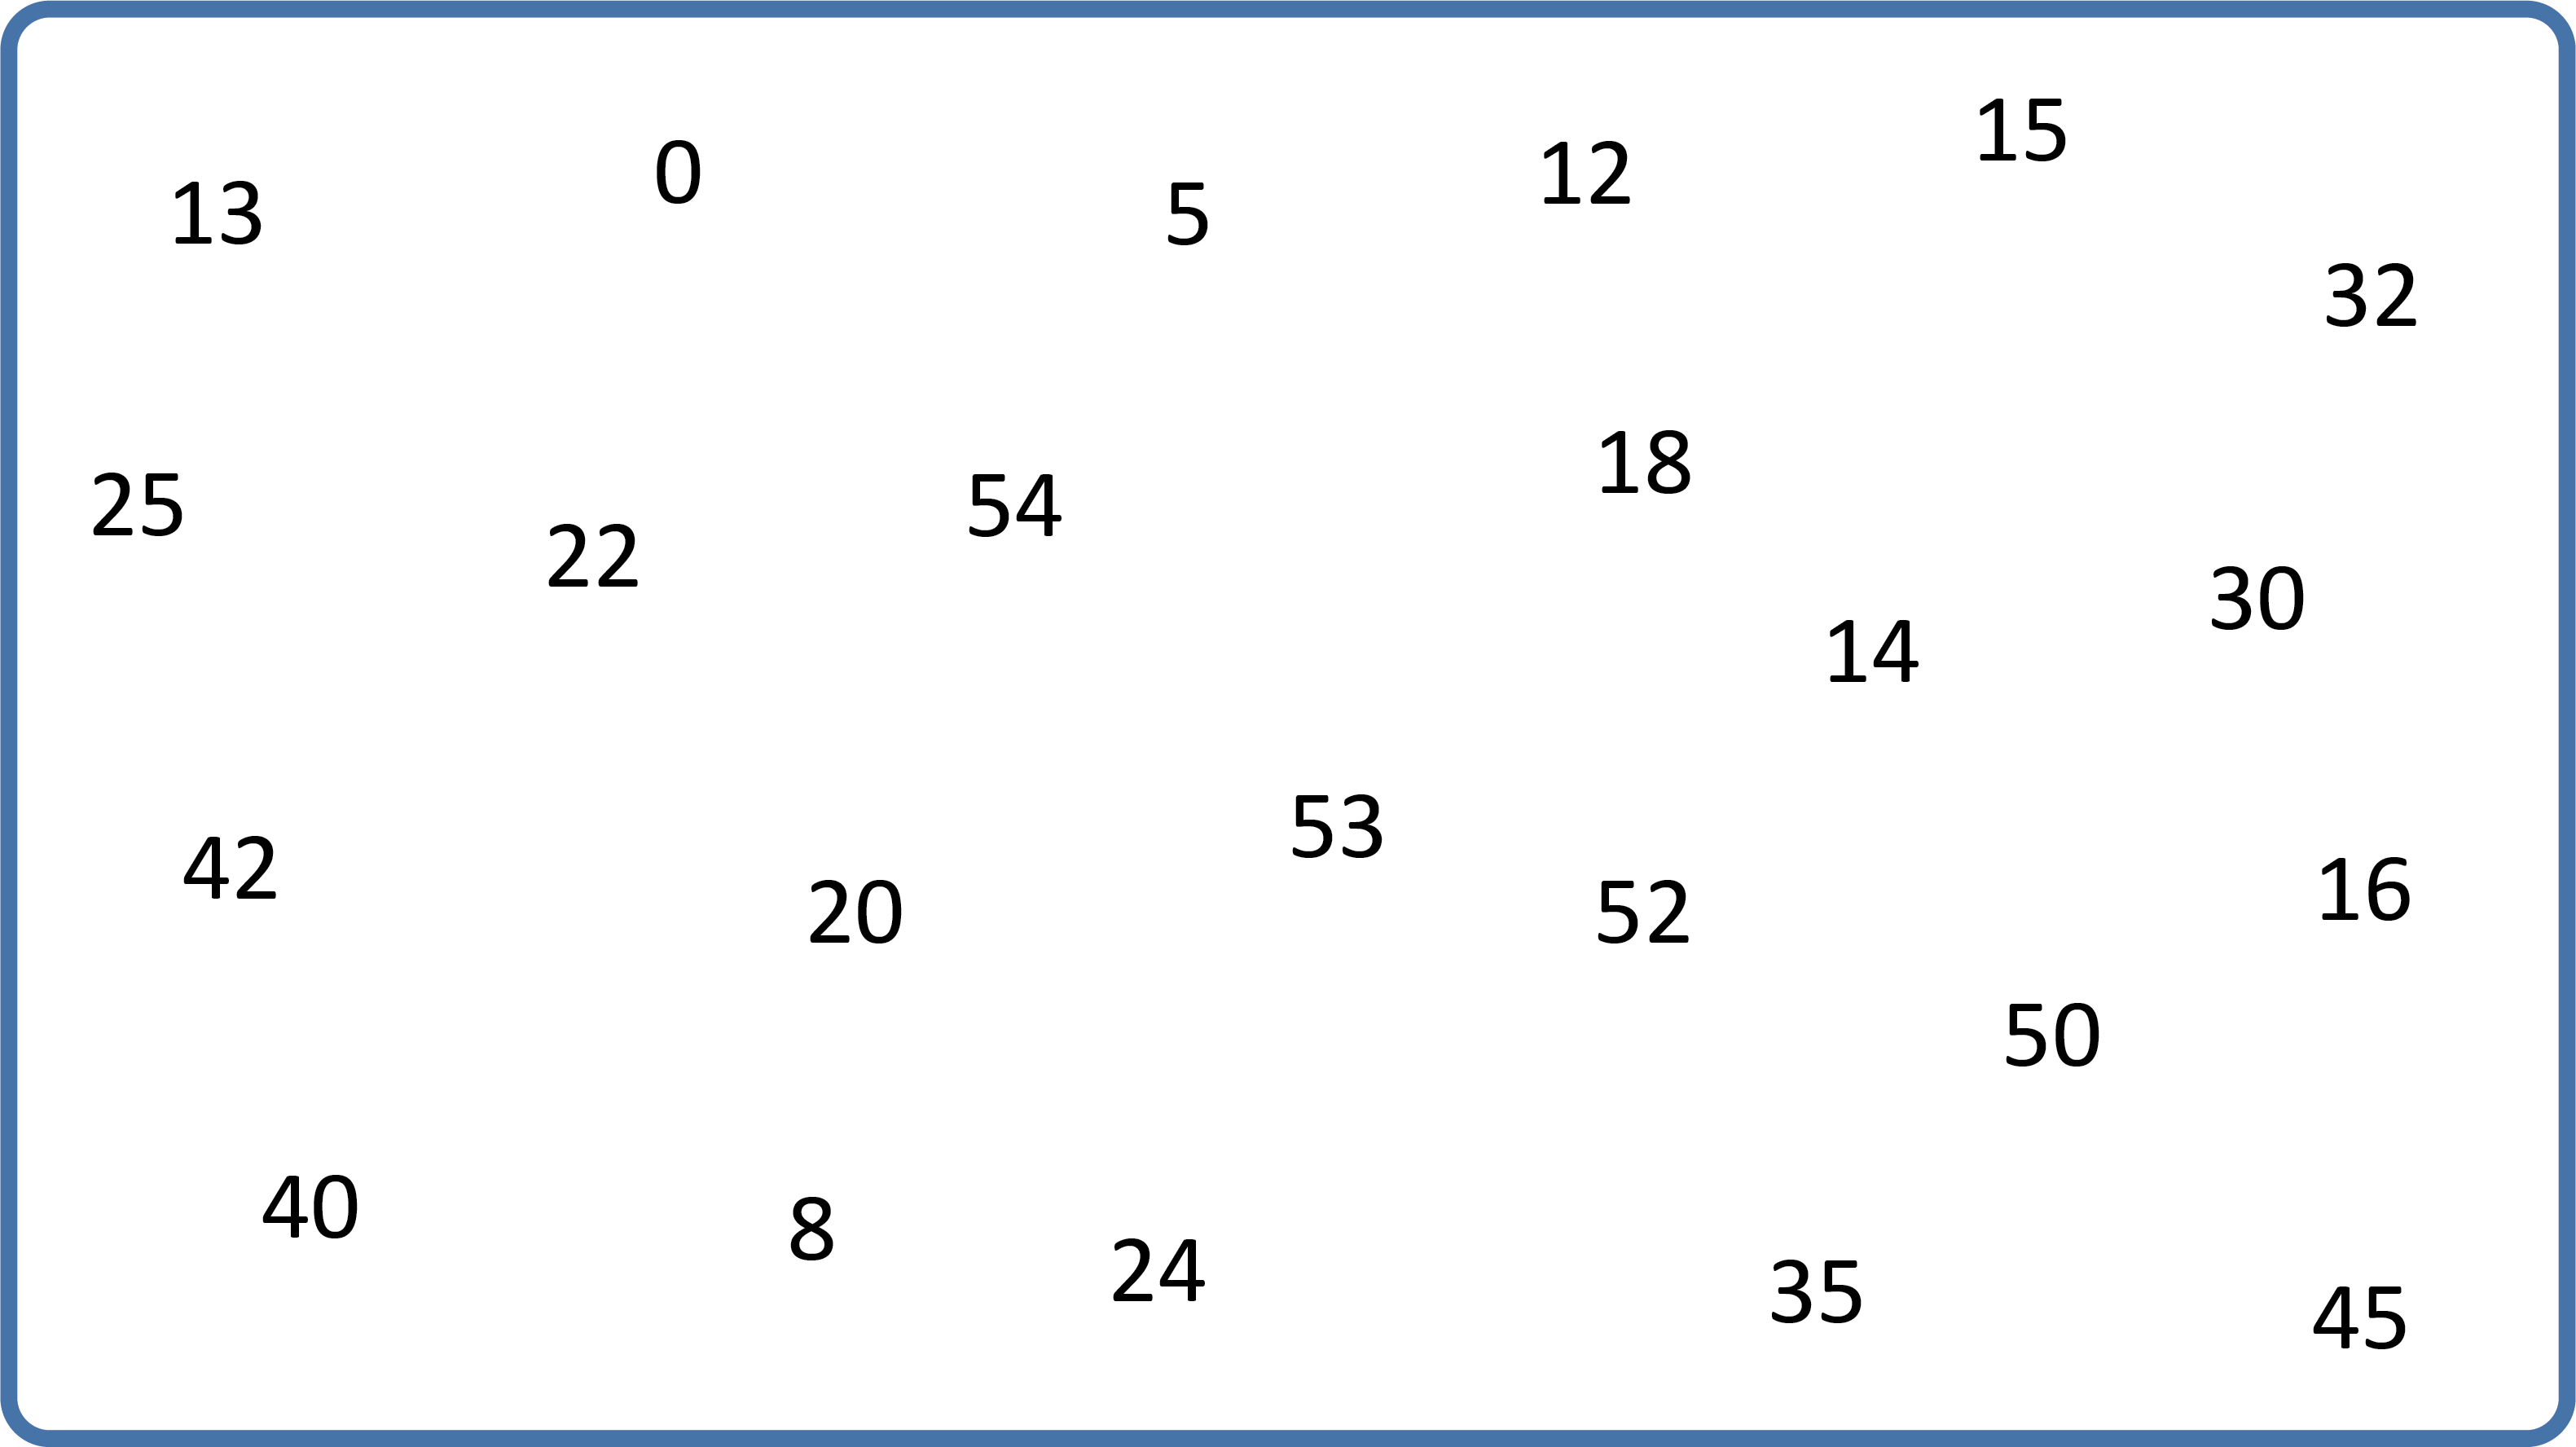
\includegraphics[width=4.51706in,height=2.09185in]{media/image25.png}

Circule aqueles que fazem parte da tabuada do 3.

\coment{12; 15; 54; 42; 24; 45.}

\colorsec{Treino}

\num{1} Uma costureira pegou uma encomenda para colocar 6 botões em
cada uma das 9 camisas que José utiliza para trabalhar. De quantos botões
ela precisará para concluir a tarefa?

\begin{minipage}{.5\textwidth}
\begin{escolha}
    \item 6
    \item 9
    \item 15
    \item 54
\end{escolha}
\end{minipage}
\sidetext{SAEB: Calcular o resultado de multiplicações ou divisões envolvendo números naturais de até 6 ordens.
BNCC: EF03MA07 – Resolver e elaborar problemas de multiplicação (por 2, 3, 4, 5 e 10) com os
significados de adição de parcelas iguais e elementos apresentados em disposição retangular,
utilizando diferentes estratégias de cálculo e registros.}

\num{2} Para uma festa familiar, a mãe de Josué comprou 12 fardos de
suco como os representados pela imagem. Pode-se considerar, então, que, para a festa, foram compradas

%Incluir imagem disponível em https://br.freepik.com/vetores-gratis/latas-em-embalagens-plasticas_11684670.htm#query=six%20pack%20soda&position=0&from_view=search&track=robertav1_2_sidr

\begin{minipage}{.5\textwidth}
\begin{escolha}
\item
  6 latas de suco.
\item
  12 latas de suco.
\item
  72 latas de suco.
\item
  144 latas de suco.
\end{escolha}
\end{minipage}
\sidetext{SAEB: Resolver problemas de multiplicação ou de divisão, envolvendo números naturais de até 6 ordens, com os significados de formação de grupos iguais (incluindo repartição equitativa e medida), proporcionalidade ou disposição retangular.
BNCC: EF03MA07 – Resolver e elaborar problemas de multiplicação (por 2, 3, 4, 5 e 10) com os
significados de adição de parcelas iguais e elementos apresentados em disposição retangular,
utilizando diferentes estratégias de cálculo e registros.}


\num{3} Um campeonato interno de basquete será promovido na escola em que Carlos
estuda. Pelas regras, cada time deverá ter 5 jogadores titulares e mais 3 reservas. Sabendo-se que serão montados 6 times, a quantidade de alunos
que poderão participar do campeonato é igual a

\begin{minipage}{.5\textwidth}
\begin{escolha}
\item
  18
\item
  30
\item
  36
\item
  48
\end{escolha}
\end{minipage}
\sidetext{SAEB: Resolver problemas de multiplicação ou de divisão, envolvendo números naturais de até 6 ordens, com os significados de formação de grupos iguais (incluindo repartição equitativa e medida), proporcionalidade ou disposição retangular.
BNCC: EF03MA07 – Resolver e elaborar problemas de multiplicação (por 2, 3, 4, 5 e 10) com os
significados de adição de parcelas iguais e elementos apresentados em disposição retangular,
utilizando diferentes estratégias de cálculo e registros.}

\chapter{Descobertas e sequências}
\markboth{Módulo 3}{}

\colorsec{Habilidades do SAEB}

\begin{itemize}
\item Inferir ou descrever atributos ou propriedades comuns que os elementos
que constituem uma sequência recursiva de números naturais apresentam.

\item Inferir o padrão ou a regularidade de uma sequência de números
naturais ordenados, objetos ou figuras.

\item Inferir os elementos ausentes em uma sequência de números naturais
ordenados, objetos ou figuras.
\end{itemize}

\coment{Habilidade da BNCC: EF03MA10.}

\conteudo{
Uma sequência ou sucessão é um conjunto numérico ordenado, no qual existe sempre uma lógica de formação.

Exemplos:

\begin{itemize}
\item
  A escalação de um time de futebol de salão em ordem alfabética:
\end{itemize}

Alan, Bruno, Fernando, Igor, Tácio.

\begin{itemize}
\item
  Sequência de números naturais pares:
\end{itemize}

(0; 2; 4; 6; 8; 10; 12; ...)

As sequências podem ser classificadas quanto ao número de elementos que apresentam ou podem apresentar.

\begin{itemize}
\item
  Finitas: sequências que apresentam um número de termos bem definido,
  ou seja, 10 termos, 20 termos, 8 termos.
\item
  Infinitas: sequências que apresentam infinitos números de termos, como a sequência dos números naturais.
\end{itemize}

Ainda podemos classificar as sequências em:

\begin{itemize}
\item
  Crescentes: aquelas em que cada termo sucessor é maior que seu antecessor.
\end{itemize}

Exemplo: (5, 10, 15, 20, 25)

\begin{itemize}
\item
  Decrescentes: aquelas em que cada termo sucessor sempre é menor do que seu antecessor.
\end{itemize}

Exemplo: (9, 7, 5, 3)

Antecessor em uma sequência numérica de números naturais: com exceção do zero,
todos os outros termos apresentam um antecessor. O antecessor é o número
imediatamente anterior àquele que está sendo analisado. Exemplo: o
antecessor de 21 é o 20, pois é o número que vem imediatamente antes do 21 na sequência dos números naturais.

Sucessor em uma sequência numérica de números naturais: todos os termos
apresentam um sucessor. O sucessor é o número que aparece imediatamente após o número que está sendo analisado. Exemplo: o sucessor de 21 é o 22, pois é o
número que vem imediatamente depois do 21 na sequência dos números naturais.
}

\colorsec{Atividades}

\num{1} A professora Mariana colocou seus alunos posicionados em uma fila, iniciada pelo aluno de tênis azul e mochila alaranjada, como na imagem.

%inserir imagem disponível em https://br.freepik.com/fotos-gratis/conjunto-de-estudio-para-criancas-diversas_18411903.htm#query=fila\%20de\%20crian\%C3\%A7as&position=12&from_view=search\&track=robertav1_2_sidr

Observe atentamente a figura e responda ao que se pede.

\begin{escolha}
\item Qual a posição na fila da criança que tem uma blusa de bolinhas coloridas?

\reduline{A criança com blusa de bolinhas coloridas está na 3º posição (terceira posição).\hfill}

\item Qual a posição na fila da criança que tem três estrelas em seu moletom?

\reduline{A criança com três estrelas no moletom está na 7º posição (sétima posição).\hfill}
\end{escolha}

\num{2} O pai de Marcelo mostrou a ele uma sequência de bolinhas pintadas com
diversas cores.

%Produzir uma imagem com essa e as cores importam. Pode ser algo bem simples, Paulo. Veja o original. Assim evitamos sobrecarga nas ilustrações.


\includegraphics[width=2.72524in,height=0.68339in]{media/image28.png}

Observando essa sequência percebemos que a bolinha pintada com a cor
verde escuro é a primeira, enquanto a bolinha pintada com a cor preta é a
última.

Quais as posições das bolinhas pintadas de cor azul?

\reduline{As bolinhas pintadas com a cor azul estão na 5º (quinta) posição e na
14º (décima quarta) posição.\hfill}

\num{3} Na prova de matemática que Manoela acabou de fazer estava o seguinte exercício:

Escreva uma sequência de números de forma crescente, de 10 em 10, começando no número 705.

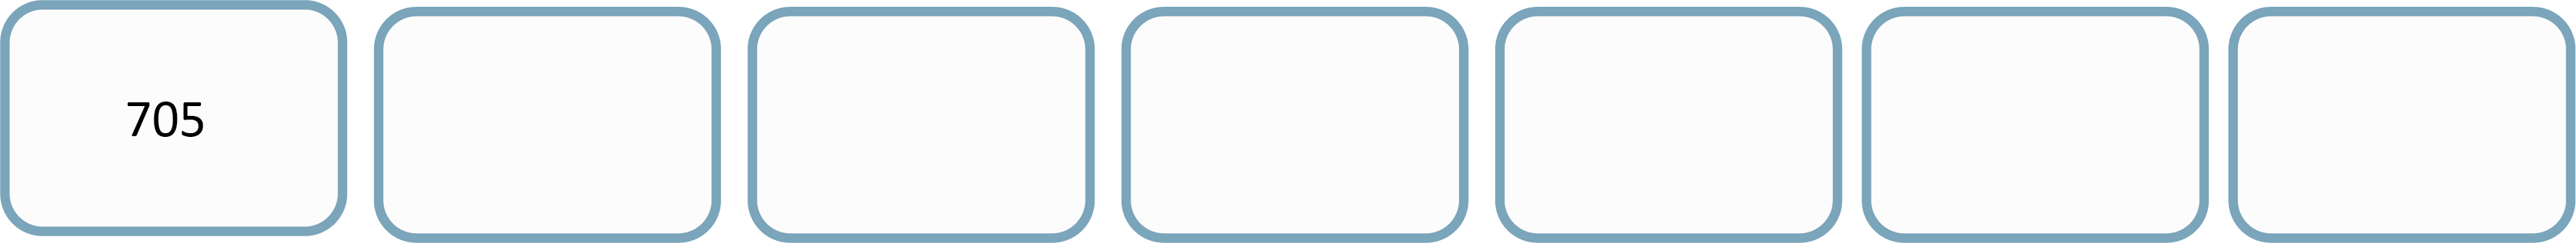
\includegraphics[width=2.95859in,height=1.10010in]{media/image29.png}

%Fazer uma figura conforme a acima, mas no lugar de 809 colocar 705. Além disso colocar os 7 retângulos na mesma linha, ou seja, um ao lado do outro
%também acho que não precisa ir para ilustração, é bem simples de fazer.

Aproveite o exercício que estava na prova de Manoela para estudar.
Escreva dentro de cada retângulo os números que completam a sequência.

\reduline{Sequência:(705; 715; 725; 735; 745; 755; 765)\hfill}

\num{4} Observe o quadro que Roberta encontrou no caderno de seu irmão.

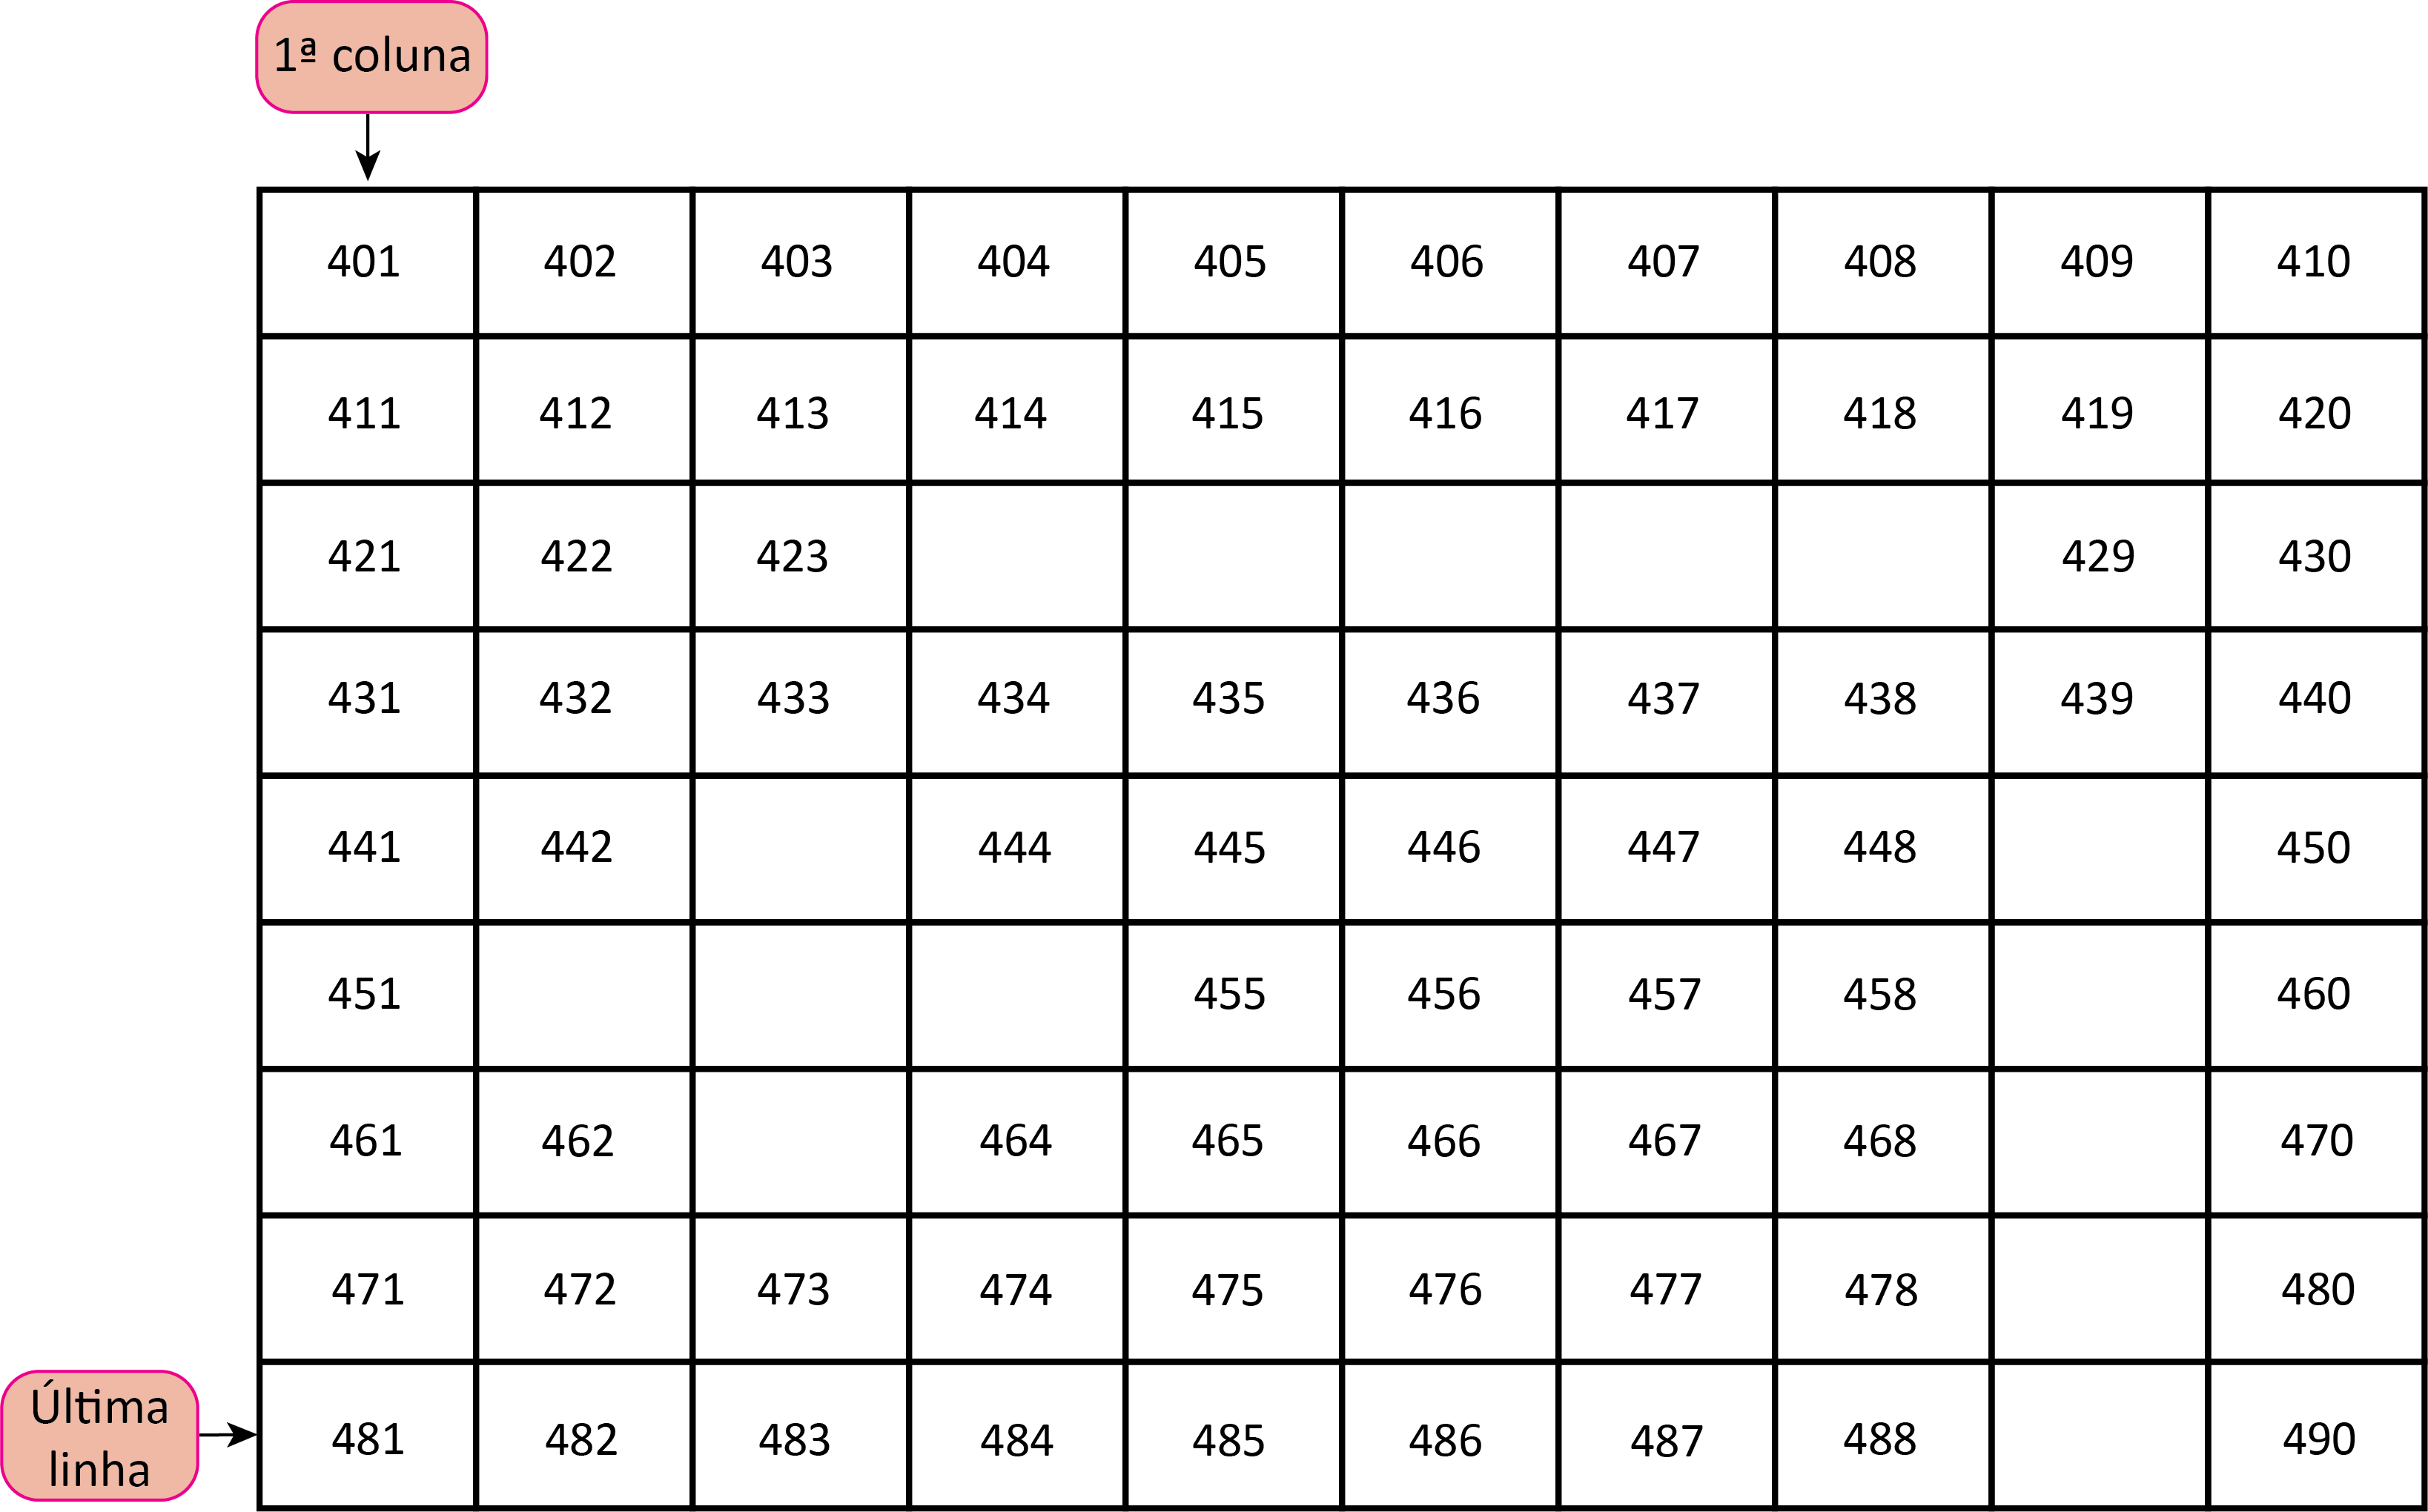
\includegraphics[width=4.05869in,height=3.09193in]{media/image30.png}

%Construir um quadro assim, nos padrões do projeto. Não precisa deixar os espaços coloridos, simplesmente deixar em branco para eles preencherem.
%Consultar o original

\begin{escolha}
\item Preencha os espaços vazios como os números que estão faltando.

\coment{424; 425; 426; 427; 428.\\
443; 449\\
452; 453; 454; 459\\
463; 469\\
479\\
489}

\item Qual o número que está na 3º coluna e na 4º linha?

\reduline{433.\hfill}

\item Qual a linha e qual a coluna em que o número quatrocentos e setenta e seis está?

\reduline{6º coluna e 8º linha.\hfill}
\end{escolha}

\num{5} Alice organizou os nomes dos amiguinhos que pretende convidar para sua
festa de aniversário em uma lista numerada.

\begin{enumerate}
\item Ana

\item Ana Clara

\item Augusto

\item Bernardo

\item Camila

\item Daniel
\end{enumerate}

Observando atentamente a lista. responda ao que se pede.

\begin{escolha}
\item Qual o nome do amigo que aparece na posição do sucessor de 4?

\reduline{Camila, pois o sucessor de 4 é o 5.\hfill}

\item Qual o nome do amigo que aparece diante do antecessor de 3?

\reduline{Ana Clara, pois o antecessor de 3 é o 2.\hfill}

\item O número diante do qual aparece o nome de Ana é antecessor de qual número?

\reduline{É Antecessor de 2, já que Ana aparece no número 1.\hfill}
\end{escolha}

\num{6} Rafaela foi a uma loja de brinquedos e, para ser atendida, pegou a senha
número 32. Todos são atendidos pela ordem numérica das senhas.

%incluir imagem disponível em https://br.freepik.com/fotos-gratis/mulher-sorridente-segurando-o-cartao-de-visita-em-branco_24488868.htm#query=senha\%20de\%20atendimento\&position=41\&from_view=search\&track=robertav1_2_sidr

\begin{escolha}
\item Qual o número da pessoa que será atendida antes de Rafaela?

\reduline{O número 31, pois é o antecessor de 32.\hfill}

\item Qual o número da pessoa que será atendida após Rafaela ser atendida?

\reduline{O número 33, pois é o sucessor de 32.\hfill}
\end{escolha}

\num{7} Observe a reta numérica com números naturais e depois responda a cada item.

%Produzir uma figura como essa, mas melhor apresentável. O número de partes e posição dos números importam.

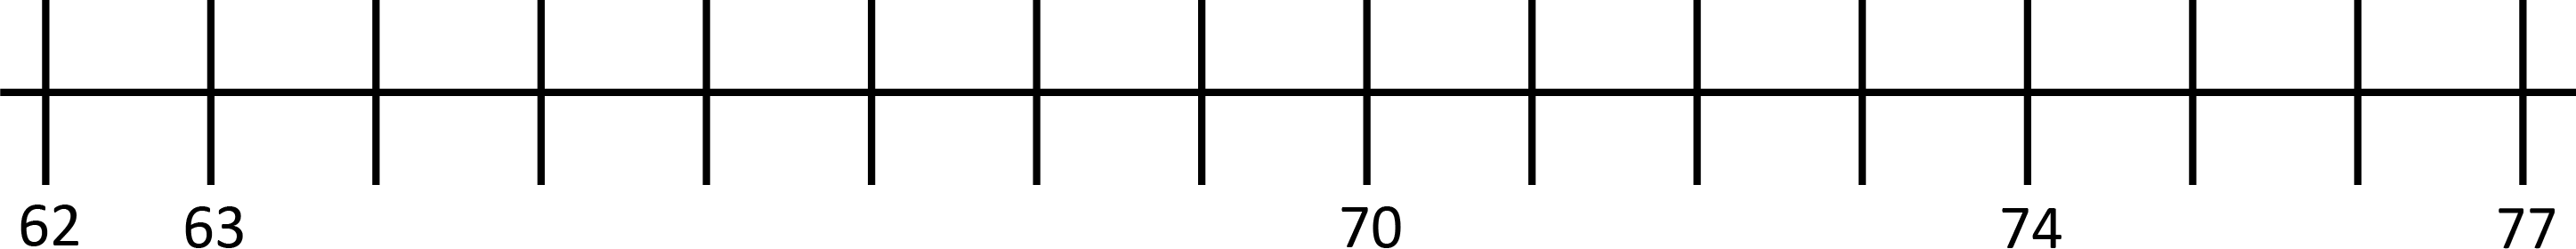
\includegraphics[width=5.22545in,height=0.75840in]{media/image31.png}

\begin{escolha}
\item Qual o número natural que será escrito imediatamente após o número 75?

\reduline{76, pois é o sucessor de 75.\hfill}

\item Qual o número natural que virá escrito antes do número 68 nessa reta numérica?

\reduline{67, pois é o antecessor de 68.\hfill}

\item Qual o antecessor do número setenta e sete?

\reduline{76\hfill}

\item Qual o sucessor do número setenta e quatro?

\reduline{75\hfill}
\end{escolha}

\num{8} Escreva os números naturais escritos em cada item em ordem crescente.

\begin{escolha}
\item 30; 25; 10; 5; 20; 15

\reduline{5; 10; 15; 20; 25; 30\hfill}

\item 7; 21; 14; 35; 28

\reduline{7; 14; 21; 28; 35\hfill}

\item 16; 8; 12; 4; 24; 20

\reduline{4; 8; 12; 16; 20; 24\hfill}
\end{escolha}

\num{9} Em cada item, indique se a sequência é crescente ou decrescente.

\begin{escolha}
\item 10; 8; 6; 4; 2; 0

\reduline{Decrescente.\hfill}

\item 10; 20; 30; 40; 50

\reduline{Crescente.\hfill}

\item 21; 19; 17; 15; 13

\reduline{Decrescente.\hfill}

\item 6; 12; 18; 24; 30; 36

\reduline{Crescente.\hfill}
\end{escolha}

\num{10} Observe as sequências dadas e determine, sem fazer desenhos, a
quantidade de bolinhas que a figura 8 de cada sequência terá.

%Paulo, acho que é possível evitar passar esta demanda pala a ilustração, já que é simples. Confira o original e avalie se é viável.

\begin{escolha}
\item \reduline{(4; 7; 10; 13; 16; 19; 22 = 25)\hfill} bolinhas

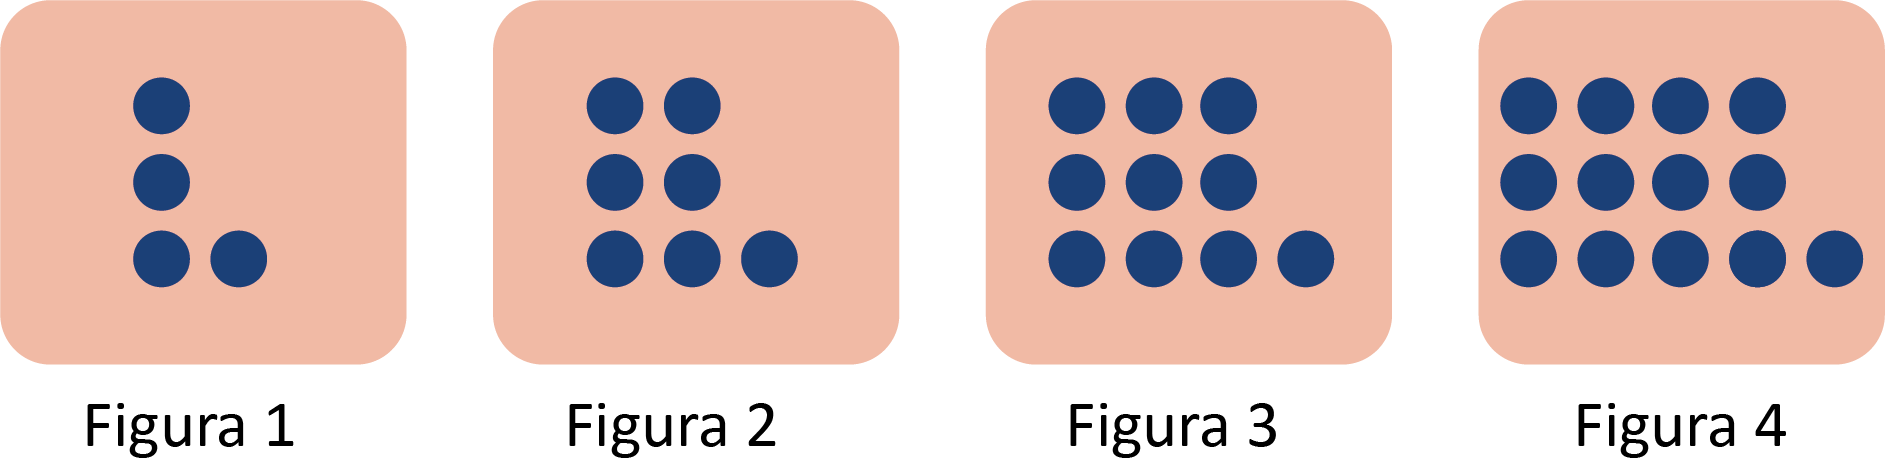
\includegraphics[width=4.09202in,height=0.85841in]{media/image32.png}

\item \reduline{(3; 6; 9; 12; 15; 18; 21 = 24)\hfill} bolinhas

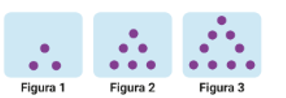
\includegraphics[width=2.38354in,height=0.81674in]{media/image33.png}

\item \reduline{(4; 8; 12; 16; 20; 24; 28 = 32)\hfill} bolinhas

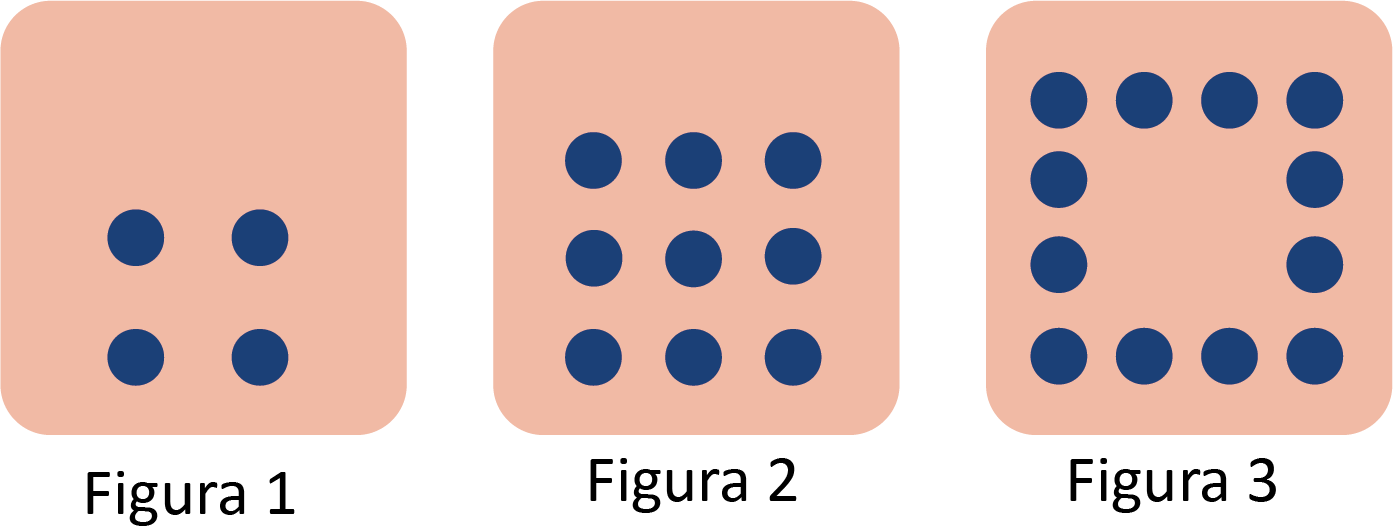
\includegraphics[width=2.38354in,height=0.85007in]{media/image34.png}

\item \reduline{(5; 10; 15; 20; 25; 30; 35 = 40)\hfill} bolinhas


\includegraphics[width=2.35854in,height=0.94175in]{media/image35.png}
\end{escolha}

\num{11} Encontre o número pedido em cada item.

\begin{escolha}
\item O sucessor de 4.089 \reduline{4.090\hfill}

\item O antecessor de 4.302 \reduline{4.301\hfill}

\item O sucessor e o antecessor do número 5.259 \reduline{5.258 e 5.260.\hfill}
\end{escolha}

\coment{Vale explorar bastante os conceitos de sucessor e antecessor com
os alunos, pois isso facilitará muitos entendimentos em anos futuros.}

\num{12} Ana Clara encontrou um papel abaixo entre os cadernos de seu irmão mais velho, com as seguintes anotações:

(21; 58; 95; 132; ...)

Ela ficou muito curiosa, pois entendeu que essa era uma sequência
numérica e queria encontrar o próximo número dessa sequência.

Ajude Ana Clara a descobrir qual é o próximo número da sequência e escreva-o no espaço disponível.

\reduline{A sequência foi montada sempre somando 37 ao número anterior para
encontrar o próximo. Portanto, o próximo número da sequência será: 132 + 37 = 169.\hfill}

\num{13} A professora de Camila decidiu propor um desafio à turma. Assim, apresentou uma sequência de figuras e pediu que os alunos descobrissem qual seria a próxima imagem. 

%Usar recortes da imagem disponível em https://br.freepik.com/vetores-gratis/cartoes-de-jogo-de-memoria-desenhados-a-mao_37451777.htm#query=sequ%C3%AAncias%20de%20figuras&position=0&from_view=search&track=robertav1_2_sidr  
%para construir a seguinte sequência:bola-quadrado-quadrado-losango-triângulo-triângulo-triângulo-oval-bola-quadrado-quadrado-losango-triângulo

Quem acertou o desafio foi o colega de Camila, Gabriel. Qual foi a resposta dele?

\reduline{Gabriel respondeu que a próxima figura seria um triângulo.\hfill}

\reduline{É possível que o aluno continue a sequência com desenhos até chegar à resposta. Não há problemas na utilização dessa técnica.\hfill}
\linhas{1}


\num{14} Observe as sequências e complete-as com os números que estão faltando.

\begin{escolha}
\item 102 \quad \reduline{104}\quad 106 \quad \reduline{108} 110 \quad \reduline{112}

\item 85 \quad \reduline{90} \quad \reduline{95} \quad 100 \quad 105 \quad \reduline{110}
\end{escolha}

\colorsec{Treino}

\num{1} Se os números escritos a seguir foram colocados em ordem crescente, qual
será o número que ficará imediatamente antes de 63?

%Colocar cada um desses números dentro de um círculo e na mesma linha.
%95; 63; 25; 76; 54; 68; 48.

\begin{minipage}{.5\textwidth}
\begin{escolha}

\item
  25
\item
  48
\item
  54
\item
  68
\end{escolha}
\end{minipage}
\sidetext{SAEB: Inferir o padrão ou a regularidade de uma sequência de números naturais ordenados, objetos ou figuras.
BNCC: EF03MA10 -- Identificar regularidades em sequências ordenadas de números naturais,
resultantes da realização de adições ou subtrações sucessivas, por um mesmo número,
descrever uma regra de formação da sequência e determinar elementos faltantes ou seguintes.}

\num{2} Observe a sequência e marque a alternativa que corresponde ao número de bolinhas que a figura 6 terá.

%Construir uma figura conforme a abaixo nos padrões do projeto
%Paulo, observando o original, acho que é possível fazer de forma bem simples as representações, sem precisar passar para a ilustração.

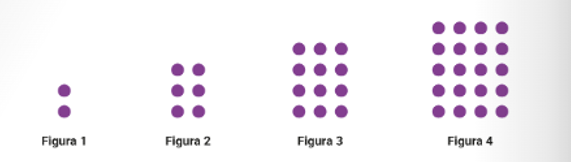
\includegraphics[width=4.75875in,height=1.35012in]{media/image37.png}

\begin{minipage}{.5\textwidth}
\begin{escolha}

\item
  25
\item
  30
\item
  35
\item
  42
\end{escolha}
\end{minipage}
\sidetext{SAEB: Inferir o padrão ou a regularidade de uma sequência de números naturais ordenados, objetos ou figuras.
BNCC: EF03MA10 -- Identificar regularidades em sequências ordenadas de números naturais,
resultantes da realização de adições ou subtrações sucessivas, por um mesmo número,
descrever uma regra de formação da sequência e determinar elementos faltantes ou seguintes.}

\num{3} Assinale a alternativa que possui uma sequência que traz um antecessor, um número e seu sucessor.

\begin{minipage}{.5\textwidth}
\begin{escolha}
\item 450 - 455 - 460

\item 526 - 626 - 726

\item 436 - 446 - 456

\item 488 - 489 - 490
\end{escolha}
\end{minipage}
\sidetext{SAEB: Inferir ou descrever atributos ou propriedades comuns que os elementos que constituem uma sequência recursiva de números naturais apresentam.
BNCC: EF03MA10 -- Identificar regularidades em sequências ordenadas de números naturais,
resultantes da realização de adições ou subtrações sucessivas, por um mesmo número,
descrever uma regra de formação da sequência e determinar elementos faltantes ou seguintes.}

\chapter{Medindo tudo}
\markboth{Módulo 4}{}


\colorsec{Habilidades do SAEB}

\begin{itemize}
\item Reconhecer a unidade de medida ou o instrumento mais apropriado para
medições de comprimento, área, massa, tempo, capacidade ou temperatura.

\item Estimar/inferir medida de comprimento, capacidade ou massa de objetos,
utilizando unidades de medida convencionais ou não ou medir comprimento,
capacidade ou massa de objetos.

\item Explicar que o resultado de uma medida depende da unidade de medida
utilizada.

\item Resolver problemas que envolvam medidas de grandezas (comprimento,
massa, tempo e capacidade) em que haja conversões entre as unidades mais
usuais.

\item Determinar o horário de início, o horário de término ou a duração de
um acontecimento.
\end{itemize}

\coment{Habilidades da BNCC: EF03MA19, EF03MA20.}

\conteudo{

%Construir os quadros abaixo seguindo o padrão de cores do material.

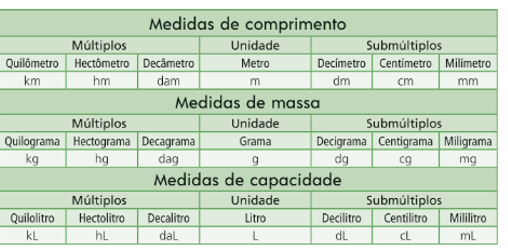
\includegraphics[width=4.23370in,height=2.06685in]{media/image39.png}

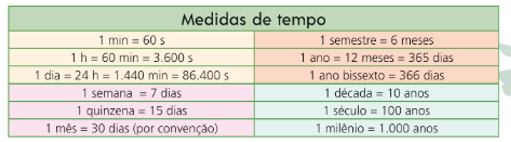
\includegraphics[width=4.25870in,height=1.18344in]{media/image40.png}
}

\colorsec{Atividades}

\num{1} Veja a imagem de uma fita métrica. Ela é utilizada para medir comprimento.

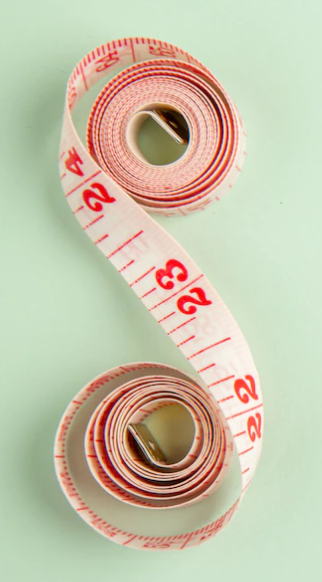
\includegraphics[width=1.29167in,height=2.33463in]{media/image41.png}

%\url{https://img.freepik.com/fotos-gratis/vista-superior-centimetro-rosa-sobre-fundo-verde_179666-22646.jpg?w=1060\&t=st=1677438557~exp=1677439157~hmac=a65357a78e180ff6d1282de8980ca1bfdad02d17329ce5b2620459dcac61e3b8}

\begin{escolha}
\item Escreva o nome de dois objetos de sua sala de aula que você acredita
  medirem menos de 1 metro.

\reduline{Resposta pessoal.\hfill}
\linhas{1}

\item Escreva o nome de dois objetos de sua sala de aula que você acredita
  medirem mais de 1 metro.

\reduline{Resposta pessoal.\hfill}
\linhas{1}
\end{escolha}

\num{2} Utilize sua régua e responda aos itens.

\begin{escolha}
\item Quantos centímetros tem o comprimento de sua borracha?

\reduline{Resposta pessoal.\hfill}
\linhas{1}

\item Qual a largura, em centímetros, da carteira que você utiliza em sua sala de aula?

\reduline{Resposta pessoal.\hfill}
\linhas{1}

\item Qual o comprimento, em centímetros, de seu lápis?

\reduline{Resposta pessoal.\hfill}
\linhas{1}

\item Qual a altura aproximada de um de seus colegas?

\reduline{Resposta pessoal.\hfill}
\linhas{1}
\end{escolha}

\num{3} Relacione a primeira com a segunda coluna levando em conta qual valor
pode corresponder à medida mostrada.

\begin{multicols}{2}
Altura aproximada de uma porta 

Comprimento aproximado de um lápis 

Comprimento médio de um quarteirão 

Comprimento aproximado de uma quadra de basquete 

\colunmbreak

20 cm

90 m

30 m

2 m
\end{escolha}

\coment{A = 2 m

B = 20 cm

C = 90 m

D = 30 m}

\num{4} Complete a frase com o número que representa quanto mede cada um dos
objetos indicados a seguir.

\begin{escolha}

\item O lápis mede \reduline{9 cm.\hfill}

  
\includegraphics[width=4.00868in,height=0.70839in]{media/image42.png}

  %O lápis na régua deve sair exatamente do 0 e chegar exatamente no 9.

\item
  A borracha mede \reduline{6 cm.\hfill}

  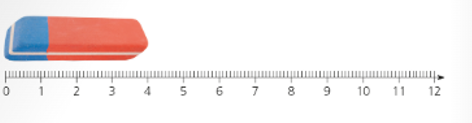
\includegraphics[width=3.93367in,height=1.02509in]{media/image43.png}

  %A borracha deve sair exatamente do zero e chegar exatamente no 6.

\item
  O apontador mede \reduline{4 cm.\hfill}

  
\includegraphics[width=3.87534in,height=0.95842in]{media/image44.png}

  %O apontador deve começar exatamente no 3 e terminar exatamente no 7.

\item
  A tesoura mede \reduline{10 cm.\hfill}

  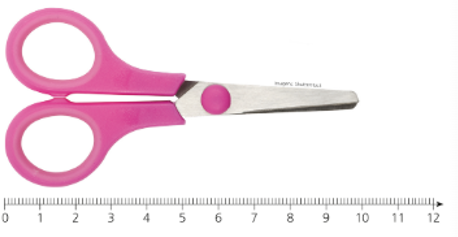
\includegraphics[width=3.81700in,height=1.97517in]{media/image45.png}

  %A tesoura deve sair exatamente do 1 e chegar exatamente no 11
  %Deixar um pedaço de linha nos locais indicados por traços nos itens acima.
\end{escolha}

\coment{Vale a pena explorar bastante essa questão de medir com o auxílio da reta
numérica, principalmente quando o início não é no zero. Esse conceito é
muito útil para entendimento de assuntos que virão em outros anos e
trabalhar bastante agora pode ajudar muito o aluno em anos posteriores.}

\num{5} Débora decidiu estimar a medida do lápis com sua borracha.

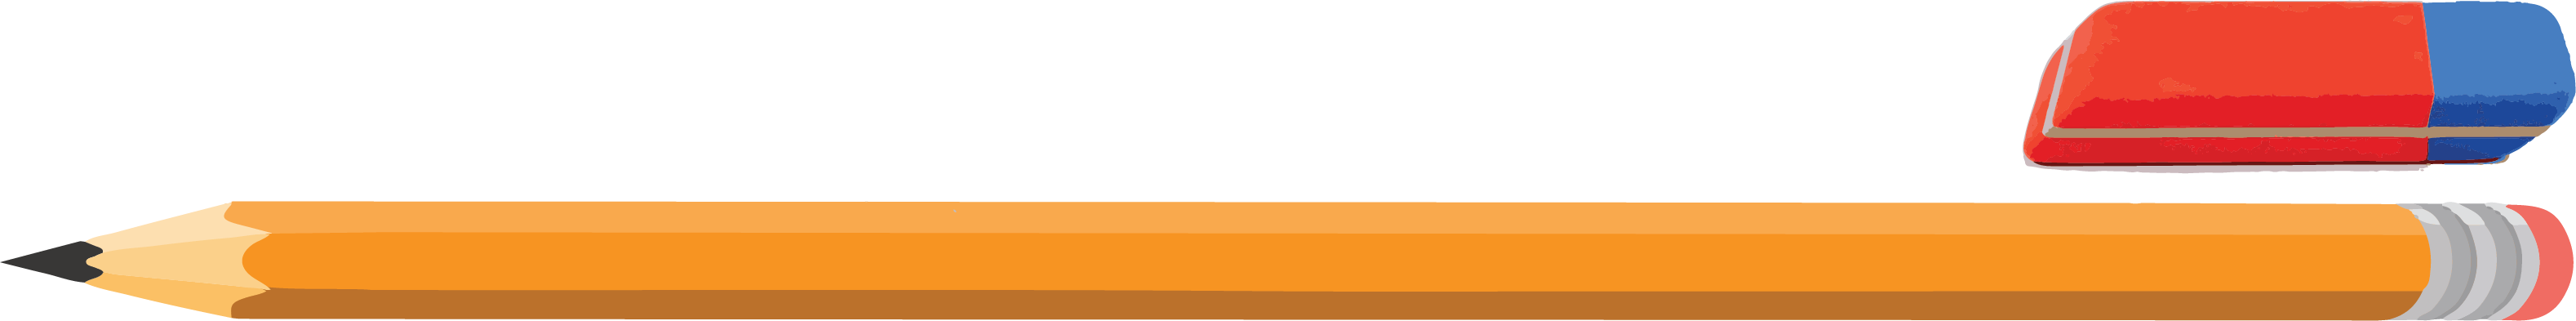
\includegraphics[width=3.84200in,height=1.23344in]{media/image46.png}

%O lápis e a borracha devem ter tamanhos de forma que no comprimento de um lápis caibam de 4 a 5 borrachas. O desenho é fundamental para a resolução dessa questão.

Quantas borrachas, aproximadamente, considerando a figura dada, mede o lápis de Débora?

\begin{minipage}{.5\textwidth}
\begin{escolha}
\item
  Entre 2 e 3.
\item
  Entre 4 e 5.
\item
  Entre 6 e 7.
\item
  Mais que 9.
\end{escolha}
\end{minipage}
\sidetext{Resposta: B
Por meio da percepção de comparação de comprimentos, percebe-se que, no
comprimento de um lápis, cabem cerca de 4 a 5 borrachas, conforme a figura dada.}

\num{6} Um dos brinquedos do parque de diversões permanente de uma cidade proíbe
que crianças com uma altura menor que 1,30 m possam brincar nessa
atração. Manoel mediu sua altura e ele está com 93 cm. Quanto ele
precisa crescer para poder realizar seu sonho de andar nesse brinquedo?

%Deixar espaço em branco equivalente a 2 linhas para cálculos

\reduline{1,30 m = 130 cm\hfill}

\reduline{130 -- 93 = 33 cm\hfill}

\reduline{Portanto, ele ainda precisará crescer 33 cm para que esteja possa aproveitar o brinquedo.\hfill}

\num{7} Roberto está com sintomas de dor de garganta e sua mãe o levou ao
médico. Chegando lá, sua temperatura foi medida e a foto do termômetro
aparece a seguir.

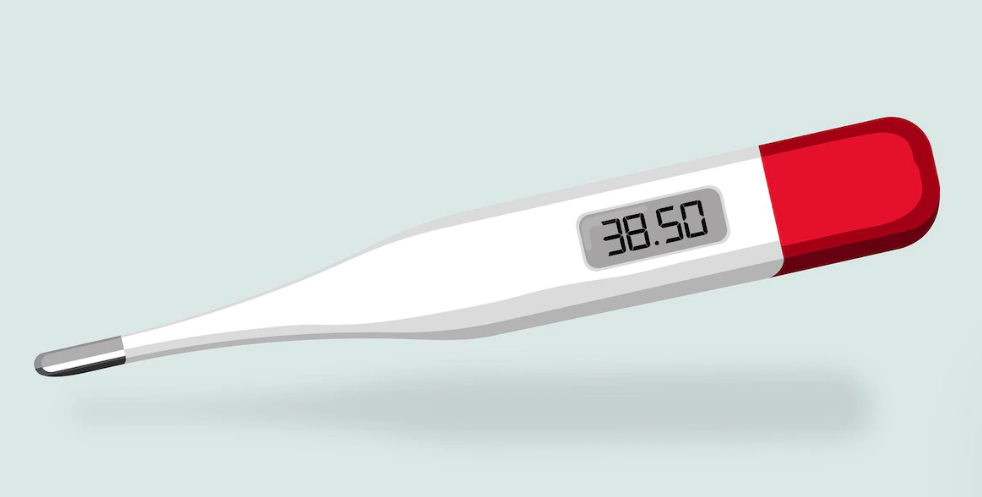
\includegraphics[width=3.15000in,height=1.59426in]{media/image47.png}

%\url{https://img.freepik.com/vetores-gratis/elemento-termometro-digital-38-5-graus-celsius_53876-119949.jpg?w=1380\&t=st=1677436599~exp=1677437199~hmac=efddbcbdae2d4d75bd1e8476eee389a985a191d57800533acdff847111e69669}

%A temperatura indicada no termômetro deve ser de 39,5º C

Analisando a imagem do termômetro, podemos concluir que a temperatura de Roberto nesse instante era de

\begin{minipage}{.5\textwidth}
\begin{escolha}

\item
  38,5º C
\item
  39º C
\item
  39,5º C
\item
  40º
\end{escolha}
\end{minipage}
\sidetext{Resposta: C
Observando a figura percebemos que o termômetro está marcando exatamente
39,5º C.}

\num{8} Para a festa de aniversário de Arthur, seu pai encomendou 24 garrafas de
refrigerante. Dessas garrafas, 10 continham, cada uma, 3 litros. Nas
demais garrafas, havia dois litros em cada uma. Com base nessas
informações, responda ao que se pede.

\begin{escolha}
\item Qual a quantidade, em mililitros, encomendada pelo pai de Arthur?

\reduline{(10 x 3) + (14 x 2) = 30 + 28 = 58 L = 58.000 ml\hfill}
\linhas{2}

\item Se cada pessoa consumiu exatamente 400 mililitros de refrigerante e
  todo o refrigerante foi consumido durante a festa, quantas pessoas
  foram ao aniversário de Arthur?

\reduline{58.000 : 400 = 145 pessoas compareceram à festa.\hfill}
\linhas{2}
\end{escolha}

\num{9} O comprimento de uma escrivaninha é de 1,6 m. Quantos palmos,
aproximadamente, mede a escrivaninha se, em média, um palmo tem 23 cm?

\begin{minipage}{.5\textwidth}
\begin{escolha}
\item
  5 palmos
\item
  6 palmos
\item
  7 palmos
\item
  8 palmos
\end{escolha}
\end{minipage}
\sidetext{Resposta: C

1,6 m = 160 cm

160 : 23 = 6,95 palmos. Aproximadamente 7 palmos.}

\num{10} Uma série de televisão produz episódios com duração de 45 minutos.
Se Jorge terminou de assistir a um episódio às 17 horas, qual foi o
horário em que ele começou a assistir ao episódio, considerando que não houve interrupções?

\reduline{Ele começou a assistir ao episódio às 16 horas e 15 minutos, pois, se a esse
horário somarmos a duração do episódio, que é de 45 minutos, teremos o
horário final, que foi às 17 horas.\hfill}

\colorsec{Treino}

\num{1}

Reinaldo foi contratado por uma empresa que tem um horário bem rígido
e semanal que deve ser cumprido corretamente. No período da manhã ele deve
cumprir 4 horas e 30 minutos de trabalho. Qual será o horário que
Reinaldo sairá para almoçar?

\begin{longtable}[]{@{}lll@{}}
\toprule
& Entrada & Saída\tabularnewline
\midrule
\endhead
Manhã & 8:00 & ?\tabularnewline
Tarde & 14:00 & 17:30\tabularnewline
\bottomrule
\end{longtable}

\begin{minipage}{.5\textwidth}
\begin{escolha}
\item
  11h00
\item
  11h30
\item
  12h00
\item
  12h30
\end{escolha}
\end{minipage}
\sidetext{SAEB: - Determinar o horário de início, o horário de término ou a duração de um acontecimento. 
BNCC: EF03MA22 -- Ler e registrar medidas e intervalos de tempo, utilizando relógios (analógico e
digital) para informar os horários de início e término de realização de uma atividade e sua
duração.}

\num{2} Júlia está com tosse e sua avó preparou para ela um chá de menta com mel que parece ser órimo para resolver o problema. A avó colocou o chá na geladeira, em garrafinhas de 500 mL. Se Júlia deve tomar um copinho de 40 mL, 4 vezes por dia, por dez dias, quantas garrafinhas precisarão ser preparadas pela avó?

\begin{minipage}{.5\textwidth}
\begin{escolha}

\item
  1
\item
  2
\item
  3
\item
  4
\end{escolha}
\end{minipage}
\sidetext{SAEB: Resolver problemas que envolvam medidas de grandezas (comprimento, massa, tempo e capacidade) em que haja conversões entre as unidades mais usuais. 
BNCC: EF03MA22 -- Ler e registrar medidas e intervalos de tempo, utilizando relógios (analógico e
digital) para informar os horários de início e término de realização de uma atividade e sua
duração.}

\num{3} Luana foi visitar sua avó, que mora em outro estado. Seu voo
saiu do aeroporto às 8 horas e 15 minutos e chegou ao seu destino às 11
horas e 30 minutos. Qual foi o tempo de duração do voo?

\begin{minipage}{.5\textwidth}
\begin{escolha}
\item
  3 horas e 15 minutos
\item
  2 horas 
\item
  2 horas e 45 minutos
\item
  3 horas e 50 minutos
\end{escolha}
\end{minipage}
\sidetext{SAEB: Resolver problemas que envolvam medidas de grandezas (comprimento, massa, tempo e capacidade) em que haja conversões entre as unidades mais usuais. 
BNCC: EF03MA22 -- Ler e registrar medidas e intervalos de tempo, utilizando relógios (analógico e
digital) para informar os horários de início e término de realização de uma atividade e sua
duração.}

\chapter{Tempo e comprimento}
\markboth{Módulo 5}{}

\colorsec{Habilidades do SAEB}

\begin{itemize}
\item Medir ou comparar perímetro ou área de figuras planas desenhadas em malha quadriculada.

\item Identificar horas em relógios analógicos ou associar horas em relógios analógicos e digitais.

\item Resolver problemas que envolvam perímetro de figuras planas.

\item Resolver problemas que envolvam área de figuras planas.
\end{itemize}

\coment{Habilidades da BNCC: EF03MA22, EF03MA23.}

\conteudo{
Semana: Uma semana é composta por 7 dias: 
Domingo
Segunda-feira
Terça-feira
Quarta-feira
Quinta-feira
Sexta-feira
Sábado


Ano: O ano é composto por 12 meses. O nome dos meses e suas respectivas quantidades de dias estão na tabela.

\begin{longtable}[]{@{}ll@{}}
\toprule
Meses que compõem o ano & Número de dias dos meses\tabularnewline
\midrule
\endhead
Janeiro & 31\tabularnewline
Fevereiro & 28 (no ano bissexto terá 29 dias)\tabularnewline
Março & 31\tabularnewline
Abril & 30\tabularnewline
Maio & 31\tabularnewline
Junho & 30\tabularnewline
Julho & 31\tabularnewline
Agosto & 31\tabularnewline
Setembro & 30\tabularnewline
Outubro & 31\tabularnewline
Novembro & 30\tabularnewline
Dezembro & 31\tabularnewline
\bottomrule
\end{longtable}

Relógio Analógico

Como é dividido: o relógio de ponteiros é dividido em 12 partes ou
seções. Você pode reparar que, da esquerda para a direita, o acessório é
numerado de 1 a 12. Esses números representam as horas.

Por sua vez, o intervalo de tempo que fica entre cada um deles
representa a contagem dos minutos. Assim, ficou convencionado que o
intervalo entre cada um deles é de 5 minutos. 


Para ver as horas em um relógio analógico, siga os seguintes passos:

Olhe para o mostrador do relógio e localize o ponteiro maior, que é o ponteiro das horas. Ele geralmente é mais curto do que o ponteiro dos minutos.

Observe a posição do ponteiro das horas. Ele estará apontando para um número que indica a hora atual. Cada número representa uma hora do dia, começando do número 1, que representa a uma hora da manhã, e terminando no número 12, que representa o meio-dia ou a meia-noite.

Observe também o ponteiro menor, que é o ponteiro dos minutos. Ele geralmente é mais comprido do que o ponteiro das horas.

Verifique a posição do ponteiro dos minutos. Ele estará apontando para um dos 60 pontos marcados no mostrador do relógio, que representam os minutos. Cada ponto representa um minuto do dia. Os números maiores podem ser úteis, porque entre cada dois deles aparecem cinco divisões de minutos. Portanto, se o ponteiro dos minutos apontar para o número 3, então basta multiplicar 5 por 3: serão 15 minutos.

Lembre-se de que, para ler as horas em um relógio analógico, é importante estar atento tanto ao ponteiro das horas quanto ao ponteiro dos minutos, a fim de obter uma leitura precisa do horário atual.
}

\colorsec{Atividades}

\num{1} Observe os horários nos relógios representados.

%Produzir imagem desses relógios com as respectivas horas indicadas

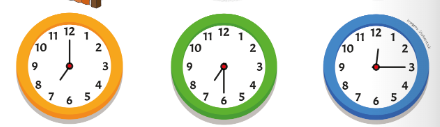
\includegraphics[width=3.66698in,height=1.05843in]{media/image51.png}

Qual o horário cada relógio está marcando?

\reduline{Primeiro relógio: sete horas\hfill}

\reduline{Segundo relógio: sete horas e trinta minutos (sete e meia)\hfill}

\reduline{Terceiro relógio: doze horas e quinze minutos (meio dia e quinze)\hfill}

\num{2} Observe o horário que os relógios digitais estão marcando:

%Produzir imagem de relógios digitais com essas horas

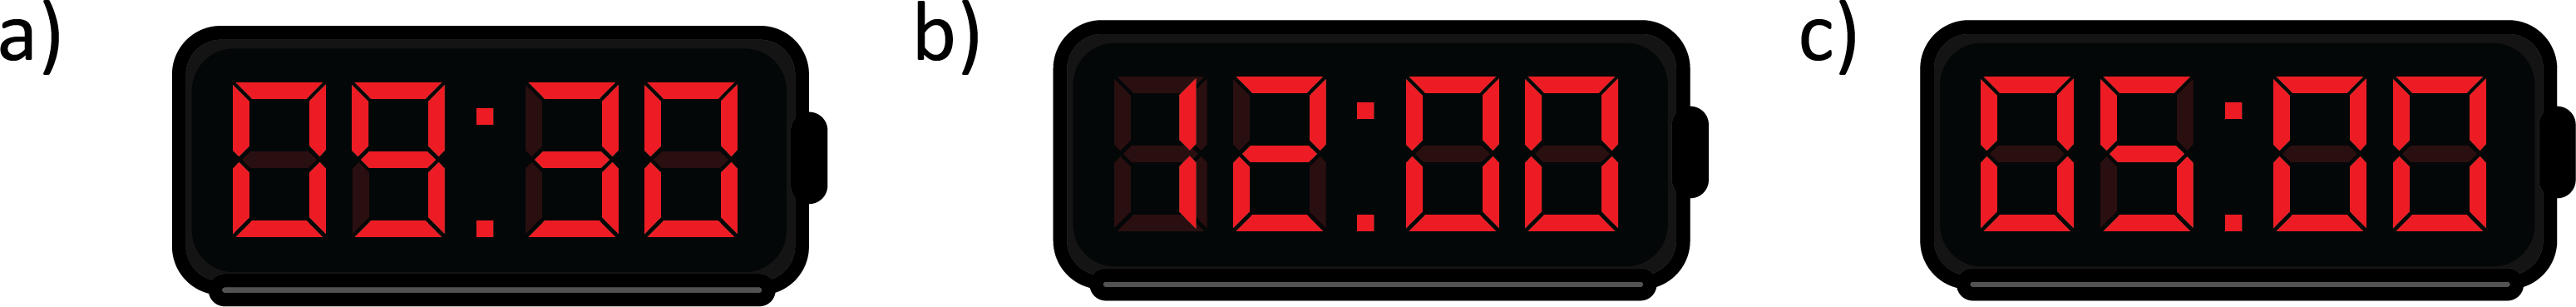
\includegraphics[width=3.54197in,height=0.29169in]{media/image52.png}

Como se lê cada um dos horários marcados?

\reduline{Nove e meia ou nove horas e trinta minutos.\hfill}

\reduline{Meio dia ou doze horas.\hfill}

\reduline{Cinco horas.\hfill}
\linhas{1}

\num{3} A professora de Francisco colocou como primeira questão da prova a seguinte imagem:

%Produzir uma imagem como essa

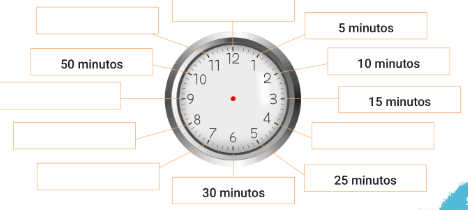
\includegraphics[width=3.90034in,height=1.75015in]{media/image53.png}

Ajude Francisco a completar os retângulos em branco com indicação de
minutos que cada um deles aponta.

\coment{20 minutos; 35 minutos; 40 minutos; 45 minutos; 55 minutos; 60 minutos.}

\num{4} Observe o calendário e em seguida responda aos itens propostos.

%Colocar uma imagem de calendário conforme essa abaixo.

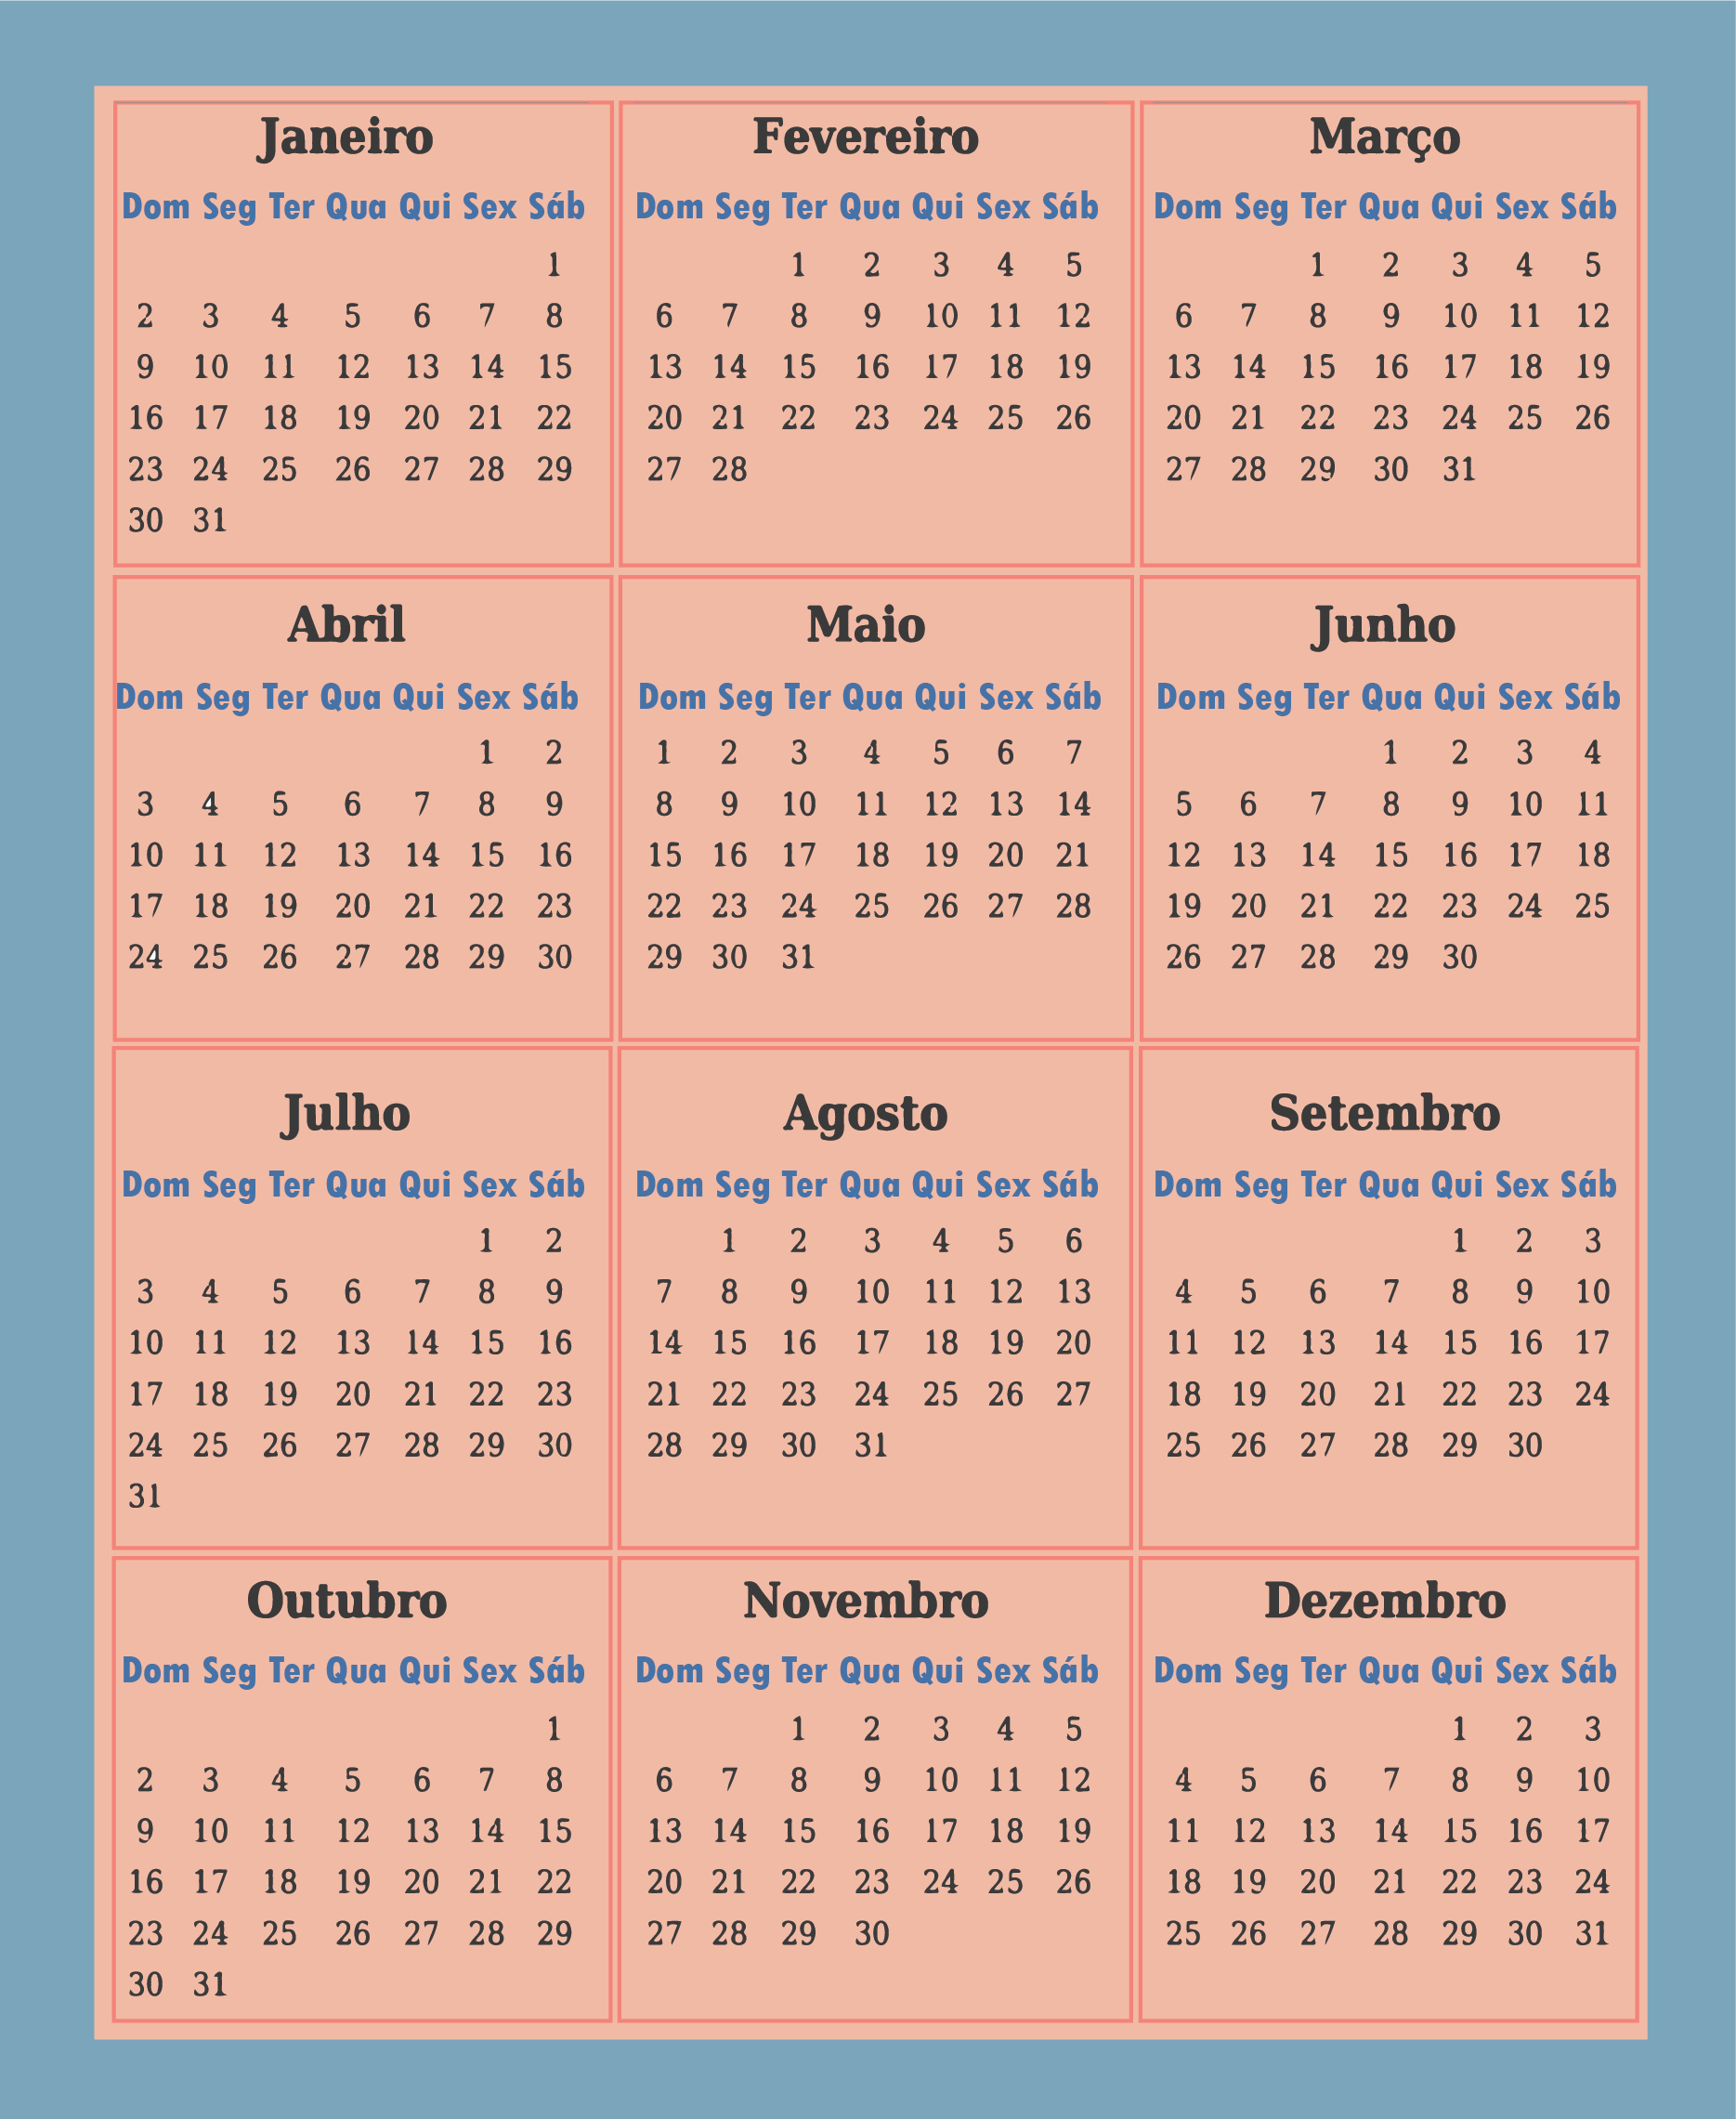
\includegraphics[width=4.13369in,height=3.20861in]{media/image54.png}

\begin{escolha}
\item Circule no calendário o dia de seu aniversário.

\reduline{Resposta pessoal.\hfill}

\item Agora, com um retângulo, marque o dia do aniversário de três colegas da sua sala.

\reduline{Resposta pessoal.\hfill}

\item Marque com um triângulo o dia do aniversário de seu professor.

\reduline{Resposta pessoal.\hfill}

\item Quantos anos você tem?

\reduline{Resposta pessoal.\hfill}

\item Você tem mais ou menos de 450 meses?

\reduline{Resposta pessoal.\hfill}
\linhas{3}
\end{escolha}

\num{5} O pai de Rafael estava conversando com um contador sobre o seu
faturamento semestral. Rafael escutou toda a conversa e depois fez os
seguintes questionamentos a seu pai:

O que é um semestre? 
Quantos semestres temos em um ano?

Diante de tantas perguntas, o pai de Rafael sentou-se com seu filho e
começou a responder aos questionamentos do filho.

Ajude o pai de Rafael a responder corretamente a todas as perguntas que o filho lhe fez.

\reduline{Um semestre é um período composto por 6 meses e em um ano temos 2 semestres.\hfill}
\linhas{4}

\num{6} Marque, desenhando no relógio analógico abaixo, os ponteiros das horas e o dos
minutos na posição exata em que estarão para representar o horário em que
suas aulas começam.

%Inserir imagem disponível em https://br.freepik.com/fotos-gratis/relogio-sem-maos_944733.htm#query=rel%C3%B3gio%20sem%20ponteiros&position=0&from_view=search&track=robertav1_2_sidr

\coment{Resposta circunstancial. Dependerá do horário de início das aulas.}


\num{7} Renato, aos finais de semana, anda de bicicleta ao redor da praça existente no bairro em que mora.

%Produzir uma imagem semelhante a abaixo

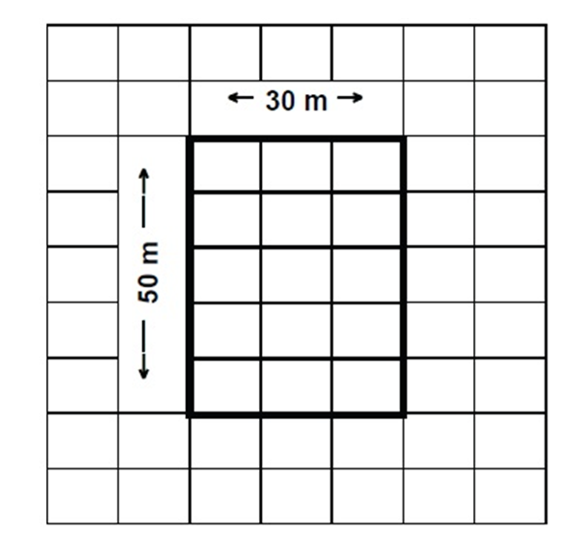
\includegraphics[width=2.35256in,height=2.20730in]{media/image55.png}

Se ele der duas voltas completas ao redor da praça, ele percorrerá qual distância?

%Deixar espaço em branco equivalente a duas linhas para cálculos

\reduline{(2 x 30 + 2 x 50) x 2 = 320 m\hfill}
\coment {Sempre que possível, estimule a montagem da expressões, para que os alunos comecem a se acostumar.}
\linhas{3}

\num{8} As figuras a seguir foram desenhadas em uma malha quadriculada.

%Produzir uma imagem semelhante a abaixo
%Cores importam

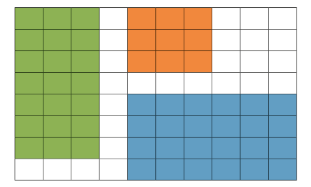
\includegraphics[width=2.59189in,height=1.55847in]{media/image56.png}

Quantos quadradinhos pintados cada figura possui?

\reduline{Verde: 21 quadradinhos.\hfill}

\reduline{Azul: 24 quadradinhos.\hfill}

\reduline{Laranja: 9 quadradinhos.\hfill}

\num{9} Os desenhos representados foram feitos com o auxílio de uma malha
quadriculada na qual cada lado de quadradinho mede 1 cm.

%Produzir uma imagem semelhante a abaixo. Cores importam

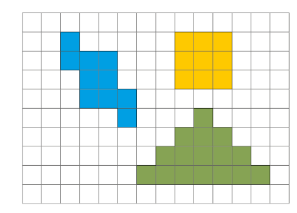
\includegraphics[width=2.47521in,height=1.77515in]{media/image57.png}

\begin{escolha}
\item Qual a medida, em centímetros, do contorno da figura azul?

\reduline{18 cm\hfill}

\item Qual a medida, em centímetros, do contorno da figura amarela?

\reduline{12 cm\hfill}

\item Qual a medida, em centímetros, do contorno da figura verde?

\reduline{22 cm\hfill}
\end{escolha}

\num{10} Utilizando sua régua, una pontos e faça uma figura na malha, representada apenas pelos pontinhos. Em seguida, mostre sua
figura para um colega e veja se ele descobre o que você representou.

%Produzir uma malha semelhante a abaixo

\includegraphics[width=4.05869in,height=1.93350in]{media/image58.png}

\coment{Resposta pessoal.}

\num{11} Observe atentamente as figuras.

%Produzir uma imagem semelhante a abaixo sem os escritos

\includegraphics[width=3.72532in,height=2.47521in]{media/image59.png}

Quais delas possuem a mesma quantidade de quadradinhos? Justifique sua resposta.

\reduline{Todas são compostas pelo mesmo número de quadradinhos.\hfill}

\num{12} Na malha quadriculada, cada quadrado representa uma área de 10 metros quadrados.

%Produzir uma imagem semelhante a abaixo

\includegraphics[width=3.33333in,height=1.50517in]{media/image60.png}

Qual a área da malha quadriculada que a figura destacada ocupa?

\reduline{Realizando a contagem de quadradinhos que preenchem a figura, chega-se à conclusão de que, para o preenchimento dela, são necessários 16 quadradinhos.\hfill}

\reduline{Portanto, 16 x 10 = 160 metros quadrados.\hfill}
\linhas{1}

\colorsec{Treino}

\num{1} Paulo resolveu ir a uma exposição e, no momento, encontra-se na
bilheteria. Quanto ele precisará andar para chegar à exposição,
considerando o caminho destacado, sabendo-se que o lado de cada
quadradinho da malha tem medida de 3m?

%Produzir uma imagem conforme abaixo. Usar imagens de banco gratuito no lugar das ilustrações, para facilitar.

\includegraphics[width=2.60897in,height=1.46587in]{media/image61.png}

\begin{minipage}{.5\textwidth}
\begin{escolha}
\item
  5 m
\item
  10 m
\item
  12 m
\item
  15 m
\end{escolha}
\end{minipage}
\sidetext{SAEB: Medir ou comparar perímetro ou área de figuras planas desenhadas em malha quadriculada. 
BNCC: EF03MA19 -- Estimar, medir e comparar comprimentos, utilizando unidades de medida
não padronizadas e padronizadas mais usuais (metro, centímetro e milímetro) e diversos
instrumentos de medida.}

\num{2} Leandro quer fazer seu nome em letras bem grandes em um papel colorido para enfeitar sua festa de aniversário. Para as letras terem tamanhos equivalentes, resolveu, primeiro, desenhá-las em um papel quadriculado. Veja o L que ele fez.

\Inserir imagem disponível em https://br.freepik.com/vetores-gratis/vetor-de-letras-de-fonte-aquarela-l_33114934.htm#page=2&query=malha%20quadriculada%20com%20letra&position=6&from_view=search&track=robertav1_2_sidr

Quantos quadrados, de forma mais aproximada, esse L ocupa?

\includegraphics[width=1.42949in,height=1.25160in]{media/image62.png}

\begin{minipage}{.5\textwidth}
\begin{escolha}
\item
  3
\item
  14
\item
  26
\item
  120
\end{escolha}
\end{minipage}
\sidetext{SAEB: Resolver problemas que envolvam área de figuras planas. 
BNCC: EF03MA19 -- Estimar, medir e comparar comprimentos, utilizando unidades de medida
não padronizadas e padronizadas mais usuais (metro, centímetro e milímetro) e diversos
instrumentos de medida.}



\num{3} Leia a notícia.

\begin{quote}
A cidade de Tombalina ganhará uma nova praça. A praça atual, com a famosa pista de corrida de 25 metros, será substituída por outra, com pista de corrida e caminhada de 125 metros de comprimento.

A nova praça será construída no centro da cidade, em uma área verde que atualmente não está sendo utilizada. A prefeitura investirá na criação de um espaço amplo e agradável para a população, com áreas de lazer e convivência.

De acordo com o prefeito da cidade, a construção da nova praça é um importante investimento para a cidade. "Estamos investindo em espaços públicos de qualidade para a população, que poderá desfrutar de um ambiente agradável e seguro para passear, praticar atividades físicas e aproveitar o tempo livre", afirmou ele.

A obra está prevista para começar em breve e deve ser concluída em alguns meses. A prefeitura pede a colaboração da população para evitar o desperdício de água e para cuidar do novo espaço, para que todos possam desfrutar de um local agradável e bonito por muitos anos.

\fonte{Texto escrito especialmente para o material.}
\end{quote}

Lendo a notícia, pode-se concluir que a nova pista de caminhada, na nova praça, será, em relação à anterior,

\begin{minipage}{.5\textwidth}
\begin{escolha}
\item
  2 vezes maior.
\item
  3 vezes maior.
\item
  4 vezes maior.
\item
  5 vezes maior.
\end{escolha}
\end{minipage}
\sidetext{SAEB: Resolver problemas que envolvam medidas de grandezas (comprimento, massa, tempo e capacidade) em que haja conversões entre as unidades mais usuais. 
BNCC: EF03MA19 -- Estimar, medir e comparar comprimentos, utilizando unidades de medida
não padronizadas e padronizadas mais usuais (metro, centímetro e milímetro) e diversos
instrumentos de medida.}


\chapter{Nosso dinheiro}
\markboth{Módulo 6}{}

\colorsec{Habilidades do SAEB}

\begin{itemize}
\item Relacionar valores de moedas e/ou cédulas do sistema monetário
brasileiro, com base nas imagens desses objetos.

\item Resolver problemas que envolvam moedas e/ou cédulas do sistema
monetário brasileiro.
\end{itemize}

\coment{Habilidade da BNCC: EF03MA24.}

\conteudo{
Conhecendo nosso dinheiro

\includegraphics[width=1.80833in,height=1.75637in]{media/image64.png}Moeda
de 5 centavos: R\$ 0,05

%\url{https://img.freepik.com/fotos-gratis/dinheiro-moedas-brasileiras-5-centavos_58702-6209.jpg?w=1060\&t=st=1677437125~exp=1677437725~hmac=c640dd9c5a2963fb4f314f44e074b714cda9416e178bd281b3d494e8262ac50e}

\includegraphics[width=1.50833in,height=1.45668in]{media/image65.png}Moeda
de 10 centavos: R\$ 0,10

\includegraphics[width=1.52500in,height=1.24749in]{media/image66.png}Moeda
de 25 centavos: R\$ 0,25

%\url{https://img.freepik.com/fotos-gratis/dinheiro-moedas-brasileiras-25-centavos_58702-6230.jpg?w=1060\&t=st=1677437194~exp=1677437794~hmac=db98c5063a731e98b23627749d52c094bab4a2f113240f1f248ee1be7074b235}

\includegraphics[width=1.56667in,height=1.61849in]{media/image67.png}Moeda
de 50 centavos: R\$ 0,50

%\url{https://img.freepik.com/fotos-gratis/dinheiro-moedas-brasileiras-50-centavos_58702-6291.jpg?w=1060\&t=st=1677437366~exp=1677437966~hmac=a914e13013ee69679658ce52473a57d18d6d23ed6356e75e5d5a34316e88cd82}

\includegraphics[width=2.11667in,height=2.01180in]{media/image68.png}Moeda
de 1 real: R\$ 1,00

%\url{https://img.freepik.com/fotos-gratis/dinheiro-moedas-brasileiras-1-real_58702-6210.jpg?w=1060\&t=st=1677437258~exp=1677437858~hmac=3314b729d5619da0bffa3b7ce7fe354ae155c324f94ca82e2cb356693ffc25dc}

\includegraphics[width=2.71068in,height=1.97500in]{media/image69.png}%Ao lado de cada nota colocar: Nota de 2 reais: R\$ 2,00; Nota de 5 reais R\$ 5,00; Nota de 10 reais: R\$ 10,00; Nota de 20 reais: R\$ 20,00. Nota de 50 reais: R\$ 50,00

%\url{https://img.freepik.com/vetores-gratis/ilustracao-gradiente-de-caixa-brasileira_52683-78831.jpg?w=996\&t=st=1677437712~exp=1677438312~hmac=c23ec28122c2591b7b261ceca09eb7c0a64059387f9729dc642986ca98524f1c}
n

\includegraphics[width=3.18285in,height=1.50833in]{media/image70.png}Nota
de 100 reais R\$ 100,00

%\url{https://img.freepik.com/fotos-premium/cem-reais-contas-dinheiro-brasileiro_499484-1535.jpg?w=1060}

\includegraphics[width=2.68333in,height=1.88913in]{media/image71.png}Nota
de 200 reais: R\$ 200,00
}

\colorsec{Atividades}

\num{1}

Complete o quadro, relacionando a imagem das cédulas e moedas do
sistema monetário brasileiro com seu valor e com como se lê esse valor.

%Colocar no espaço da cédula ou moeda a foto das seguintes notas

\begin{longtable}[]{@{}lll@{}}
\toprule
Cédula ou moeda & Valor & Como se lê\tabularnewline
\midrule
\endhead
Foto nota 200 reais & & Duzentos reais\tabularnewline
Foto nota 100 reais & &\tabularnewline
Foto nota 50 reais & &\tabularnewline
Foto de 20 reais & R\$ 20,00 &\tabularnewline
Foto de 10 reais & &\tabularnewline
Foto de 5 reais & & Cinco reais\tabularnewline
Foto nota 2 reais & &\tabularnewline
Foto moeda de 1 real & &\tabularnewline
Foto moeda de 0,50 centavos & R\$ 0,50 &\tabularnewline
Foto moeda de 0,25 centavos & &\tabularnewline
Foto moeda de 0,10 centavos & &\tabularnewline
Foto moeda de 0,05 centavos & & Cinco centavos\tabularnewline
\bottomrule
\end{longtable}

Resposta:

\begin{longtable}[]{@{}lll@{}}
\toprule
Cédula ou moeda & Valor & Como se lê\tabularnewline
\midrule
\endhead
Foto nota 200 reais & R\$ 200,00 & Duzentos reais\tabularnewline
Foto nota 100 reais & R\$ 100,00 & Cem reais\tabularnewline
Foto nota 50 reais & R\$ 50,00 & Cinquenta reais\tabularnewline
Foto de 20 reais & R\$ 20,00 & Vinte reais\tabularnewline
Foto de 10 reais & R\$ 10,00 & Dez reais\tabularnewline
Foto de 5 reais & R\$ 10,00 & Cinco reais\tabularnewline
Foto nota 2 reais & R\$ 2,00 & Dois reais\tabularnewline
Foto moeda de 1 real & R\$ 1,00 & Um real\tabularnewline
Foto moeda de 0,50 centavos & R\$ 0,50 & Cinquenta
centavos\tabularnewline
Foto moeda de 0,25 centavos & R\$ 0,25 & Vinte e cinco
centavos\tabularnewline
Foto moeda de 0,10 centavos & R\$ 0,10 & Dez centavos\tabularnewline
Foto moeda de 0,05 centavos & R\$0,05 & Cinco centavos\tabularnewline
\bottomrule
\end{longtable}

\num{2} André foi ao banco efetuar um saque (retirada de dinheiro de sua conta
bancária) e, ao pegar o valor pretendido, recebeu as seguintes cédulas e moedas:

%Produzir uma figura conforme a abaixo mantendo as quantidades das notas

\includegraphics[width=2.50022in,height=1.34178in]{media/image72.png}
\includegraphics[width=2.26686in,height=0.87508in]{media/image73.png}

Qual o valor que André retirou de sua conta bancária?

\reduline{1 x 50 + 4 x 20 + 1 x 10 + 3 x 5 + 2 x 2 + 2 x 1 + 4 x 0,50 = 50 + 80 +
10 + 15 + 4 + 2 + 2 = R\$ 173,00.\hfill}
\linhas{2}

\num{3} A mãe de Leonardo foi a supermercado e comprou os seguintes produtos:

%Produzir uma imagem como a abaixo mantendo valores e quantidades

\includegraphics[width=4.10036in,height=1.22511in]{media/image74.png}

Observando o preço pago por cada produto e a quantidade que ela comprou de cada um, pode-se afirmar que o gasto dela no supermercado foi igual a:

\begin{minipage}{.5\textwidth}
\begin{escolha}

\item
  R\$ 35,00
\item
  R\$ 42,00
\item
  R\$ 61,00
\item
  R\$ 67,00
\end{escolha}
\end{minipage}
\sidetext{Resposta: D.
Açúcar: R\$: 5,00\\
Suco: 3 x 3 = R\$ 9,00\\
Arroz: R\$ 10,00\\
Queijo: 19,00\\
Manteiga: R\$ 15,00\\
Café: R\$ 9,00\\
Valor total: 5 + 9 + 10 + 19 + 15 + 9 = R\$ 67,00}

\num{4} Uma grande rede de lojas realizou uma promoção de vendas após o Natal.
Veja os produtos que estavam em promoção e seus respectivos preços.

%Produzir uma imagem como abaixo mantendo os valores. Usar imagens de banco gratuito e inserir os preços, para facilitar. Seguem links de banco com cada produto:

%Airfryer: https://br.freepik.com/fotos-premium/maquina-de-fritadeira-de-ar-na-cozinha_16446672.htm#query=airfryer&position=28&from_view=search&track=robertav1_2_sidr

%Fogão: https://br.freepik.com/vetores-gratis/placa-de-inducao-com-forno-fogao-eletrico-frontal-e-vista-superior_13009313.htm#page=2&query=stove&position=25&from_view=search&track=robertav1_2_sidr

%Microondas: https://br.freepik.com/fotos-premium/forno-de-micro-ondas-isolado-no-branco_7357543.htm#query=microwave&position=40&from_view=search&track=robertav1_2_sidr

%Liquidificador: https://br.freepik.com/fotos-premium/liquidificador-eletrico-isolado-no-branco-close-up_8273323.htm#query=liquidificador&position=13&from_view=search&track=robertav1_2_sidr

Observavdo a figura, responda a cada item.

\begin{escolha}
\item Se uma pessoa comprar um fogão e um liquidificador, quanto irá pagar?

\reduline{1.300 + 250 = R\$ 1.550,00.\hfill}
\linhas{2}

\item Se uma pessoa conseguir um desconto de R\$ 50,00 para pagamento à
  vista na compra do microondas, qual será o valor que ela pagará?

\reduline{480 -- 50 = R\$ 430,00.\hfill}
\linhas{2}
\end{escolha}

\num{5} A tabela a seguir mostra a pesquisa de preços que José está fazendo
sobre um jogo de videogame e um controle bluetooth.

\begin{longtable}[]{@{}lll@{}}
\toprule
Produto & Loja A & Loja B\tabularnewline
\midrule
\endhead
Jogo de vdeogame & R\$ 200,00 & R\$ 176,00\tabularnewline
Controle bluetooth & R\$ 616,00 & R\$ 654,00\tabularnewline
total & &\tabularnewline
\bottomrule
\end{longtable}

\begin{escolha}
\item Se José comprar os dois itens na loja A, pagará quanto?

\reduline{200 + 616 = R\$ 816,00\hfill}
\linhas{2}

\item Se optar por comprar tuda na loja B, qual o valor que pagará?

\reduline{176 + 654 = R\$ 830,00\hfill}
\linhas{2}

\item Se ele quer pagar o menor preço possível, determine em qual loja ele
  deverá comprar cada item e calcule qual o valor que pagará.

\reduline{Ele deverá comprar o jogo na loja B por R\$ 176,00 e o controle na
  loja A por R\$ 616,00. Com isso, pagará R\$ 792,00.\hfill}
  \linhas{1}
\end{escolha}

\num{6} Marta foi à papelaria comprar uma caneta de que estava precisando para
continuar seus estudos. Ela comprou uma caneta que custava 7 reais e 75
centavos. Sabendo-se que ela pagou com uma nota de 10 reais, quais
cédulas e moedas ela recebeu de troco?

\reduline{Como o enunciado indica que são cédulas e moedas, ela deva ter recebido
de troco uma nota de 2 reais e 1 moeda de 25 centavos.
Existem outras opções que podem ser exploradas.
Explorar com os alunos outras situações para que treinem um
pouco esse conceito. Além disso, converse um pouco com os alunos sobre
outras moedas que existem no mundo e qual o seu valor em relação ao real
e vice-versa.\hfill}

\num{7} Caíque economizou muito dinheiro, pois queria comprar um videogame usado
que custava R\$ 3.490,00 à vista. Ele conversou com o vendedor, pediu
um desconto extra e foi atendido com um desconto de R\$ 350,00. Quanto ele pagou pelo videogame?

\reduline{R\$ 3.490,00 -- R\$ 350,00 = R\$ 3.140,00\hfill}
\linhas{2}

\num{8} Em muitas compras a prazo é exigida uma entrada que é paga no ato da
compra e o restante do valor pode ser dividido em um número combinado de
parcelas mensais. Veja o exemplo.

\includegraphics[width=2.90025in,height=0.89174in]{media/image76.png}

%Produzir uma imagem como acima. O escrito deve ser: Entrada R\$ 25 000,00 e o restante dividido em 36 parcelas de R\$ 1 200,00 cada uma.
%a imagem disponível em https://br.freepik.com/fotos-premium/sinal-de-banner-publicitario-em-branco-no-teto-do-carro_16098885.htm#query=car%20add%20mockup&position=25&from_view=search&track=robertav1_2_sidr pode ser aproveitada para a produção da ilustração.

\begin{escolha}
\item Qual o valor que será dividido em 24 vezes?

\reduline{24 x 1.200 = R\$ 28.800,00\hfill}
\linhas{2}

\item Qual o valor que cada parcela terá?

\reduline{Lendo atentamente o texto, sabe-se que cada parcela será de R\$ 1.200,00\hfill}
\linhas{2}

\item Se à vista a loja fornece um desconto de R\$ 2.580,00, quem optar por
  pagar à vista pagará quanto pelo carro?

\reduline{25.000 + (24 x 1.200) -- 2.580 = R\$ 51.220,00\hfill}
\linhas{2}
\end{escolha}

\coment{Incentive os alunos a fazer a montagem da expressão, mesmo que
encontrem outra saída de resolução. É importante não inibir outras resoluções,
mas sim mostrar várias formas e, dentre elas, a montagem da expressão.}

\num{9}  Complete os quadros com as quantidades de cada nota para que se
obtenham os valores estipulados.

\begin{escolha}

\item
  %Produzir uma figura como essa
\includegraphics[width=4.14203in,height=1.14177in]{media/image77.png}
%No lugar de R\$ 836,00 colocar R\$ 966,00


\item
  %Produzir uma imagem com essa
\includegraphics[width=4.10036in,height=1.20844in]{media/image78.png}
%Deixar só o valor R\$ 3 940,00 e deletar o de R\$ 1 700,00
\end{escolha}

\coment{
Podem surgir outras combinações para a resposta. Incentive e
estimule essa criatividade.
A) Uma possibilidade para R\$ 966,00 podem ser 48 notas de 20 reais e 3
  notas de 2 reais.
B) Uma possibilidade para R\$ 3.940,00 podem ser 15 notas de 200 reais, 9
  notas de 100 reais e 2 notas 20 reais.}

\num{10} Bianca foi a uma loja comprar um presente para sua filha e se deparou
com os seguintes objetos e seus respectivos preços:

%Produzir uma imagem como essa mantendo os valores abaixo.

\includegraphics[width=3.51697in,height=1.08343in]{media/image80.png}

Observe atentamente a figura e, em seguida, responda a cada um dos itens.

\begin{escolha}
\item Qual dos três objetos é o mais barato?

\reduline{O mais barato é o pião mecânico, no valor de R\$ 50,00.\hfill}
\linhas{1}

\item Se Bianca resolveu comprar o patinete e o relógio, quanto ela gastou?

\reduline{250 + 154 = R\$ 404,00\hfill}
\linhas{1}
\end{escolha}

\num{11} Jonas recebe R\$ 350,00 por semana. Na segunda-feira gastou 100 reais
com a conta de luz; na terça-feira, 50 reais com transporte e, na quarta-feira, 120 reais com comida. Quanto sobrou para ele gastar nos outros
dias que ainda faltam para acabar a semana?

\reduline{350 -- 100 -- 50 -- 120 = 350 -- 270 = R\$ 80,00\hfill}
\linhas{2}

\colorsec{Treino}

\num{1} Felipe, vendo alguns anúncios de televisores na internet, encontrou um que dizia:

%Produzir uma imagem com essa mantendo os valores. Usar imagem de banco gratuito como base.

\includegraphics[width=1.95850in,height=0.77507in]{media/image81.png}

Uma pessoa que quiser aproveitar o desconto oferecido irá pagar nessa TV

\begin{minipage}{.5\textwidth}
\begin{escolha}
\item
  R\$ 985,00.
\item
  R\$ 75,00.
\item
  R\$ 910,00.
\item
  R\$ 1.060,00.
\end{escolha}
\end{minipage}
\sidetext{SAEB: Resolver problemas que envolvam moedas e/ou cédulas do sistema monetário brasileiro. 
BNCC: EF03MA24 -- Resolver e elaborar problemas que envolvam a comparação e a equivalência de
valores monetários do sistema brasileiro em situações de compra, venda e troca.}

\num{2} Júlia irá trocar suas notas por moedas para guardar tudo em seu
cofrinho. Ela quer trocar suas notas por moedas de 1 real. Marque a
alternativa que traz o número correto de moedas de 1 real que ela
irá receber pelas suas notas quando efetuar a troca.

%Produzir imagens como as abaixo mantendo os valores

\includegraphics[width=3.34196in,height=0.88341in]{media/image82.png}

\begin{escolha}
\item
\includegraphics[width=1.93350in,height=0.50004in]{media/image83.png}

\item
\includegraphics[width=1.26678in,height=0.72506in]{media/image84.png}

\item
\includegraphics[width=1.95850in,height=0.69173in]{media/image85.png}

\item
\includegraphics[width=1.95850in,height=0.69173in]{media/image85.png}\includegraphics[width=1.26678in,height=0.72506in]{media/image84.png}
\end{escolha}

\coment{SAEB: Resolver problemas que envolvam moedas e/ou cédulas do sistema monetário brasileiro. 
BNCC: EF03MA24 -- Resolver e elaborar problemas que envolvam a comparação e a equivalência de
valores monetários do sistema brasileiro em situações de compra, venda e troca.}

\num{3} Na lanchonete a que Augusto costuma ir com seus amigos se encontra a
seguinte tabela de preços:

\begin{longtable}[]{@{}ll@{}}
\toprule
Produtos & Valor por unidade\tabularnewline
\midrule
\endhead
Pão de queijo & R\$ 3,00\tabularnewline
Bombom & R\$ 5,00\tabularnewline
Suco & R\$ 6,00\tabularnewline
Doce & R\$ 4,50\tabularnewline
Refrigerante & R\$ 4,50\tabularnewline
Cachorro-quente & R\$ 12,00\tabularnewline
\bottomrule
\end{longtable}

Na última vez que Augusto foi a esse lugar, ele comprou 1 bombom, 2
sucos e 2 cachorros-quentes. Qual o valor gasto por Augusto nesse dia?

\begin{minipage}{.5\textwidth}
\begin{escolha}

\item
  R\$ 18,00
\item
  R\$ 28,00
\item
  R\$ 30,00
\item
  R\$ 41,00
\end{escolha}
\end{minipage}
\sidetext{SAEB: Resolver problemas que envolvam moedas e/ou cédulas do sistema monetário brasileiro. 
BNCC: EF03MA24 -- Resolver e elaborar problemas que envolvam a comparação e a equivalência de
valores monetários do sistema brasileiro em situações de compra, venda e troca.}

\chapter{Qual é a chance?}
\markboth{Módulo 7}{}

\colorsec{Habilidades do SAEB}

\begin{itemize}
\item Identificar, entre eventos aleatórios, aqueles que têm menos, maiores ou
iguais chances de ocorrência, sem utilizar frações.

\item Determinar a probabilidade de ocorrência de um resultado em eventos
aleatórios, quando todos os resultados possíveis têm a mesma chance de
ocorrer (equiprováveis).
\end{itemize}

\coment{Habilidade da BNCC: EF03MA25.}

\conteudo{
PROBABILIDADE: é uma razão entre o que se espera ou se deseja que aconteça e o total
possível de possibilidades. Essa probabilidade indica
a chance de determinado resultado ocorrer. O número 0 representa uma
probabilidade de zero em cada cem, ou seja, chance nenhuma de o resultado ocorrer;
o número 1 corresponde à probabilidade cem em cada cem, o que quer
dizer que será certeza de que o evento ocorrerá.
}

\colorsec{Atividades}

\num{1} Em um estojo há 25 lápis coloridos e 18 lápis pretos. Retirando-se, ao
acaso, um lápis desse estojo, o que tem chance maior: retirar um lápis
colorido ou um lápis preto? Justifique sua resposta.

\reduline{Como há mais lápis coloridos do que pretos no estojo, a maior chance
quando se retira um único lápis desse estojo é a de que saia um lápis
colorido.\hfill}

\reduline{Professor, aproveite o exercício para dar outros exemplos e, aos poucos,
ir trabalhando o conceito com os alunos, devido à importância de eles
desenvolverem essa habilidade de encontrar maiores chances por meio de uma análise simples.\hfill}

\num{2} Daniel joga um dado de seis faces, numeradas de 1 a 6, que não foi modificado e funciona perfeitamente. Calcule a probabilidade de Daniel passar pelas seguintes situações.

\begin{escolha}
\item Tirar, na face voltada para cima, um número par.

\reduline{Temos 6 possibilidades de números que podem sair: 1, 2, 3, 4, 5 e 6. Interessa, nesse caso, um número par: 2, 4 e 6. Portanto a probabilidade será de metade das chances, ou seja, de uma em cada duas.\hfill}

\item Tirar, na face voltada para cima, um número ímpar.

\reduline{Temos 6 possibilidades de números que podem sair: 1, 2, 3, 4, 5 e 6. Interessa, nesse caso, um número par: 1, 3 e 5. Portanto a probabilidade será de metade das chances, ou seja, de uma em cada duas.\hfill}

\item Tirar, na face voltada para cima, um número menor do que 3.

\reduline{Temos 6 possibilidades de números que podem sair: 1, 2, 3, 4, 5 e 6. Interessa, nesse caso, um número menor que 3: 1 e 2. Portanto a probabilidade é de uma em cada três.\hfill}
\end{escolha}



\num{3} Uma sacola escura, que não permite visualizar o que tem dentro, contém
20 bolas idênticas, mas de cores diferentes. Sabe-se que 6 são azuis, 8
são pretas, 4 são vermelhas e 2 são amarelas. Retirando-se uma bola ao
acaso:

\begin{escolha}
\item Qual cor de bola tem mais chances de sair?

\reduline{A maior chance é de sair uma bola preta.\hfill}
\linhas{1}

\item  Qual cor de bola tem menos chances de sair?

\reduline{A menor chance é de sair uma bola amarela.\hfill}
\linhas{1}
\end{escolha}

\coment{Deixe bem claro que a probabilidade máxima de algo
acontecer e 100 em cada cem, assim como a mínima é de zero em cada cem.}

\num{4} Lucas tem guardados, em uma caixa, 10 livros de matemática, 5 de história, 3 de inglês e
2 de geografia. Retirando-se um desses itens, ao acaso, da caixa,
responda:

\begin{escolha}
\item Qual a chance de ser um livro?

\reduline{A chance é tota, ou seja, de 100 em 100, já que há apenas livros na caixa.\hfill}
\linhas{1}

\item  Qual a probabilidade de ser um livro de português?

\reduline{A probabilidade é de 1 em cada 2, ou metade, ou 50 em cada 100.\hfill}
\linhas{1}
\end{escolha}

\num{5} Na sala em que Clarissa estuda há 32 alunos, dos quais 8 são meninas. A
professora irá escolher um aluno para verificar se este fez a tarefa.
Qual a probabilidade de um menino ser escolhido?

\reduline{Total de alunos: 32\hfill}

\reduline{Número de meninos: 32 -- 8 = 24\hfill}

\reduline{Portanto, a probabilidade será de 24 em cada 32, ou seja, 3 em cada 4.\hfill}


\num{6} Uma letra é escolhida ao acaso dentre as que formam a palavra
FUNDAMENTO. A probabilidade de essa letra ser uma vogam é maior ou menor do que a de ser uma consoante?

\reduline{Total de letras: 10\hfill}

\reduline{Vogais: 4; consoantes: 6.\hfill}

\reduline{Portanto, a probabilidade de ser uma vogal é menor do que a de ser uma consoante.\hfill}


\num{7} Um baralho convencional é composto por 52 cartas divididas em quatro
naipes (copas, paus, ouros e espadas) sendo 13 de cada naipe. Dessa
forma, se retirarmos uma carta ao acaso, qual a probabilidade de sair
uma carta do naipe de copas?

\reduline{Total de cartas: 52\hfill}

\reduline{Carta de copas: 13\hfill}

\reduline{Probabilidade = 13 em 52 = uma em cada quatro.}\hfill

\num{8} Vítor quer escolher um número para sua camiseta do time de futebol e ele
pode escolher qualquer número de 1 a 16. Qual a probabilidade de que ele
escolha um número maior que 8 e menor que 14?

\reduline{Total de números: 16\hfill}

\reduline{Total de números que interessam: 5 (9, 10, 11, 12 e 13)\hfill}

\reduline{Probabilidade de cinco em dezesseis.}\hfill

\num{9} Os 450 estudantes de um colégio responderam a uma pergunta sobre qual a
sua área de conhecimento preferida, entre Exatas, Humanidades e
Biológicas. As respostas foram computadas e alguns dados foram colocados
na tabela.

\begin{longtable}[]{@{}ll@{}}
\toprule
Área & Sexo\tabularnewline
& Masculino (M)\tabularnewline
Exatas (E) & 200\tabularnewline
Humanas (H) & 150\tabularnewline
Biológicas (B) & 100\tabularnewline
Total & 265\tabularnewline
\bottomrule
\end{longtable}

Um estudante é escolhido ao acaso. Determine a probabilidade de esse
estudante preferir humanas.

\reduline{Total de estudantes: 450\hfill}

\reduline{Preferência por humanas: 150\hfill}

\reduline{Probabilidade: 450/150 = 3 = uma chance em cada três.\hfill}


\num{10} Carlos possui duas urnas com bolas que só são diferenciadas pela cor. A
distribuição das bolas nas urnas e por cor se encontra na tabela a
seguir.

\begin{longtable}[]{@{}lll@{}}
\toprule
Cor & Urna 1 & Urna 2\tabularnewline
\midrule
\endhead
Amarela & 4 & 0\tabularnewline
Azul & 3 & 1\tabularnewline
Branca & 2 & 2\tabularnewline
Verde & 1 & 3\tabularnewline
Vermelha & 0 & 4\tabularnewline
\bottomrule
\end{longtable}

Ele irá colocar todas as bolas dessas duas urnas em uma única urna 3. Em
seguida retirará uma bola, ao acaso, dessa última urna. Qual a
probabilidade de que ele retire uma bola verde?

\reduline{Total de bolas: 20\hfill}

\reduline{Bolas verdes: 4\hfill}

\reduline{Probabilidade: 4 em cada 20, ou 1 em cada 5, ou 25 em cada 100.\hfill}


\colorsec{Treino}

\num{1} Mateus precisa tem uma coleção de carrinhos em miniatura. No total, ele tem 30 carrinhos, sendo 10 caminhões (metade deles com 4 rodas e a outra metade com 6 rodas), 15 carrinhos conversíveis e 5 jipes. Se ele pegar um dos carrinhos de olhos fechados, sem escolher, para dar de presente ao seu irmão, quais são as chances de ser um caminhão de 6 rodas?

\begin{minipage}{.5\textwidth}
\begin{escolha}
\item
  dez em cada trinta.
\item
  cinco em cada trinta.
\item
  um em cada trinta.
\item
  trinta em cada trinta.
\end{escolha}
\end{minipage}
\sidetext{SAEB: Identificar, entre eventos aleatórios, aqueles que têm menos, maiores ou iguais chances de ocorrência, sem utilizar frações. 
BNCC: EF03MA25 -- Identificar, em eventos familiares aleatórios, todos os resultados possíveis,
estimando os que têm maiores ou menores chances de ocorrência.}



\num{2} Em uma festa a fantasia temática de alimentação, onde há 100 convidados, apareceram as seguintes fantasias:

Maçã - 12
Batata frita - 20
Cacho de uva - 8
Frango assado - 31
Bolacha - 9
Bolo - 7
Kiwi - 10
Cachorro-quente - 3

Se uma dessas pessoas for escolhida, aleatoriamente, para ganhar um prêmio, qual a chance de ela estar fantasiada de fruta?

\begin{minipage}{.5\textwidth}
\begin{escolha}
\item
30 em cada 100.
\item
50 em cada 100.
\item
Nenhuma chance.
\item
Chance total, de 100 em cada 100.
\end{escolha}
\end{minipage}
\sidetext{SAEB: Determinar a probabilidade de ocorrência de um resultado em eventos aleatórios, quando todos os resultados possíveis têm a mesma chance de ocorrer (equiprováveis).  
BNCC: EF03MA25 -- Identificar, em eventos familiares aleatórios, todos os resultados possíveis,
estimando os que têm maiores ou menores chances de ocorrência.}



\num{3} Uma turma de terceiro ano tem 23 alunos. Três deles, Ana, Carlos e Tatiana, se candidataram para serem representantes de turma. Nessa votação, cada aluno só pode votar uma vez e os candidatos não votam. Veja a lista de chamada, com os primeiros nomes dos alunos, dessa turma.

\begin{enumerate}
\item Abigail

\item Ana

\item Aparecida

\item Bernardo

\item Carla

\item Carlos

\item Coralina

\item Daniel 

\item Elena

\item Estêvão

\item Gustavo

\item Helena

\item Hilda

\item Ingrid

\item Janaína

\item Joaquim

\item Juarez

\item Manuel

\item Nina

\item Paula

\item Pedro

\item Rafael

\item Tatiana
\end{enumerte}

Imagine que a professora sorteie um aluno, de forma aleatória, para ser o primeiro a votar. Quais as chances de esse primeiro votante ter o nome iniciado com a mesma letra de um dos nomes dos candidatos?

\begin{minipage}{.5\textwidth}
\begin{escolha}
\item
3 em 20
\item
4 em 20
\item
7 em 20
\item
Nenhuma chance.
\end{escolha}
\end{minipage}
\sidetext{SAEB: Determinar a probabilidade de ocorrência de um resultado em eventos aleatórios, quando todos os resultados possíveis têm a mesma chance de ocorrer (equiprováveis). 
BNCC: EF03MA25 -- Identificar, em eventos familiares aleatórios, todos os resultados possíveis,
estimando os que têm maiores ou menores chances de ocorrência.}

\chapter{Dados e gráficos}
\markboth{Módulo 8}{}

\colorsec{Habilidades do SAEB}

\begin{itemize}
\item Ler/identificar ou comparar dados estatísticos expressos em tabelas
(simples ou de dupla entrada).

\item Ler/identificar ou comparar dados estatísticos expressos em gráficos
(barras simples ou agrupadas, colunas simples ou agrupadas, pictóricos
ou de linhas).

\item Resolver problemas que envolvam dados apresentados tabelas (simples ou
de dupla entrada) ou gráficos estatísticos (barras simples ou agrupadas,
colunas simples ou agrupadas, pictóricos ou de linhas).
\end{itemize}

\coment{Habilidade da BNCC: EF03MA27.}

\conteudo{
Tipos de gráficos mais utilizados em estatística:

\begin{itemize}
\item
  Gráfico de colunas ou barras
\end{itemize}

%Usar a imagem disponível em https://br.freepik.com/vetores-gratis/conjunto-de-elementos-planos-de-graficos_9387088.htm#query=graphic&position=6&from_view=search&track=sph
%Inserir os seguintes gráficos da figura: linha 1 coluna 1, linha 4 coluna 1, linha 4 coluna 4.


\begin{itemize}
\item
  Pictograma
\end{itemize}

%Fazer a figura abaixo nos moldes do projeto.

Além disso ao invés de raparigas colocar meninas e no lugar de rapazes
colocar meninos.

\includegraphics[width=4.18370in,height=2.21686in]{media/image89.png}

\begin{itemize}
\item
  Gráfico de linhas
\end{itemize}

%Usar a imagem disponível em https://br.freepik.com/vetores-gratis/conjunto-de-elementos-planos-de-graficos_9387088.htm#query=graphic&position=6&from_view=search&track=sph
%Inserir os seguintes gráficos da figura: linha 2 coluna 1, linha 3 coluna 4.


\begin{itemize}
\item
  Gráfico de setores
\end{itemize}

%Usar a imagem disponível em https://br.freepik.com/vetores-gratis/conjunto-de-elementos-planos-de-graficos_9387088.htm#query=graphic&position=6&from_view=search&track=sph
%Inserir os seguintes gráficos da figura: linha 2 coluna 4, linha 3 coluna 3.
}

\colorsec{Atividades}

\num{1} Após um longo período de férias as aulas de Regina voltaram a acontecer.
No primeiro dia de aula a professora fez uma pesquisa sobre as viagens de seus alunos nas férias. Cada aluno foi
orientado a escolher somente um lugar e, após escutar todas as respostas,
a professora montou o seguinte gráfico sobre a pesquisa:

\includegraphics[width=4.23077in,height=2.15071in]{media/image92.png}

Qual foi a resposta menos dada pelos alunos segundo esse gráfico?

\begin{minipage}{.5\textwidth}
\begin{escolha}
\item
  Casa
\item
  Fazenda do tio
\item
  Praia
\item
  Sítio da vovó
\end{escolha}
\end{minipage}
\sidetext{Resposta: B

Observando o gráfico, percebemos que a resposta que menos apareceu foi a
fazenda do tio, com 5 aparições.}

\num{2} Durante uma aula de matemática sobre estatística, os alunos fizeram uma
pesquisa entre eles para consolidar seus aprendizados. A turma fez uma
pergunta a todos os alunos sobre o tipo de filme preferido e cada aluno
poderia dar apenas uma resposta. Após essa coleta de respostas, eles
fizeram a tabela mostrando as respostas dos meninos e das
meninas:

\includegraphics[width=3.42308in,height=1.97646in]{media/image93.png}

%Construir uma tabela com os seguintes valores em colunas:

\begin{multicols}{2}
6 

4

6

1

\columnbreak

15

2

1

1
\end{multicols}

Observando a tabela, conclui-se que o tipo de filme de que as meninas menos
gostam é

\begin{minipage}{.5\textwidth}
\begin{escolha}

\item
  Aventura.
\item
  Comédia.
\item
  Desenho animado.
\item
  Terror.
\end{escolha}
\end{minipage}
\sidetext{Resposta: D

Pela análise da tabela, conclui-se que o tipo de filme de que as meninas menos gostam é o de terror, com 1 voto.}

\num{3} Após todas as rodadas de um campeonato de futebol, os organizadores
apresentaram um gráfico sobre o número de pontos ganhos por cada
time.

\includegraphics[width=3.19194in,height=2.04184in]{media/image94.png}

Observando atentamente o gráfico, podemos concluir que o time D fez

\begin{minipage}{.5\textwidth}
\begin{escolha}
\item
  50 pontos.
\item
  40 pontos.
\item
  35 pontos.
\item
  30 pontos.
\end{escolha}
\end{minipage}
\sidetext{Resposta: A
Olhando atentamente para o gráfico, temos que o time D fez 50 pontos
durante esse campeonato.}

\num{4} Durante um evento de automobilismo, foram colhidas as informações sobre o número de carros
que entraram e também a quantidade de pessoas que estavam em cada carro.
Esses dados foram colocados em uma tabela.

\begin{longtable}[]{@{}ll@{}}
\toprule
Número de pessoas por carro & Quantidade de carros\tabularnewline
\midrule
\endhead
Apenas 1 pessoa & 5\tabularnewline
2 pessoas & 12\tabularnewline
3 pessoas & 15\tabularnewline
4 pessoas & 7\tabularnewline
5 pessoas & 5\tabularnewline
\bottomrule
\end{longtable}

Construa um gráfico de colunas com os dados da tabela.

%Produzir uma figura como essa.

\includegraphics[width=4.76708in,height=3.21695in]{media/image95.png}

%Resposta:
%\includegraphics[width=4.76708in,height=3.21695in]{media/image95.png}

\num{5} Uma empresa de telefonia fez uma pesquisa para saber o índice de
satisfação de seus clientes em relação aos serviços prestados. Esses dados foram
colocados em uma tabela.

%Produzir uma figura semelhante a essa

\includegraphics[width=4.92543in,height=1.97517in]{media/image96.png}

Pela análise do gráfico, pode-se afirmar que o número de pessoas que
responderem Bom ou Normal foi

\begin{minipage}{.5\textwidth}
\begin{escolha}
\item
  120.
\item
  270.
\item
  330.
\item
  500.
\end{escolha}
\end{minipage}
\sidetext{Resposta: B\\
Bom: 120\\
Normal: 150\\
Total: 270}

\num{6} A tabela mostra a quantidade de abacaxis vendidos por um feirante
durante alguns dias do mês de maio.

\begin{longtable}[]{@{}ll@{}}
\toprule
Dia & Quantidade de abacaxis vendidos\tabularnewline
\midrule
\endhead
04/05 & 89\tabularnewline
05/05 & 68\tabularnewline
06/05 & 52\tabularnewline
07/05 & 71\tabularnewline
\bottomrule
\end{longtable}

Analisando os dados da tabela, responda ao que se pede em cada item.

\begin{escolha}
\item Quantos abacaxis foram vendidos nos dias 05/05 e 06/05?
  
\reduline{68 + 52 = 120\hfill}
\linhas{1}

\item Em que dia a venda de abacaxis foi a maior?
  
\reduline{O dia com maior venda foi 04/05, com 89 abacaxis.\hfill}
\linhas{1}

\item Em que dia a venda de abacaxis foi a menor?
  
\reduline{O dia com menor venda foi 06/05, com 52 abacaxis.\hfill}
\linhas{1}
\end{escolha}

\num{7} Uma empresa de doces resolveu contratar um matemático que realizasse uma
pesquisa para verificar o tipo preferido de sobremesa das pessoas que
frequentavam determinado supermercado. Os entrevistados poderiam dar
apenas uma resposta dentre as oferecidas na pesquisa e, após contagem dos
votos sobre a preferência, o matemático apresentou o gráfico a seguir
para a empresa que o contratou.

\begin{longtable}[]{@{}ll@{}}
\toprule
Sobremesa & Total de votos\tabularnewline
\midrule
\endhead
Pudim & 35\tabularnewline
Sorvete & 20\tabularnewline
Doce de leite & 22\tabularnewline
Goiabada com queijo & 10\tabularnewline
Salada de frutas & 13\tabularnewline
\bottomrule
\end{longtable}

Analisando o gráfico apresentado, responda:

\begin{escolha}
\item Qual a sobremesa menos votada?

\reduline{A sobremesa menos votada foi a goiabada com queijo.\hfill}

\item Qual a sobremesa mais votada?

\reduline{A sobremesa mais votada foi o pudim.\hfill}

\item Construa uma sequência crescente dos números apresentados na tabela.

\reduline{10;13;20;22;35.\hfill}

\item Após construir a sequência crescente, qual número ficou na posição central?

\reduline{O número que ocupa a posição central na sequência é o 20.\hfill}
\end{escolha}

\num{8} O professor de educação física apresentou os dados da quantidade de gols
marcados pelos 4 times que dispuraram o interclasses de futebol no ano
corrente.

%Produzir um gráfico como essa nos moldes do projeto. Não alterar valores.

\includegraphics[width=3.30769in,height=1.97201in]{media/image97.png}

Analisando atentamente o gráfico, responda:

\begin{escolha}
\item Qual turma fez a maior quantidade de gols? E qual foi a quantidade que fizeram?

\reduline{A turma que fez a maior quantidade de gols foi a B, com 9 gols.\hfill}

\item Quais turmas fizeram um número de gols maior que 6?

\reduline{As turmas que fizeram um número de gols maior que 6 foram as turmas B
  e D. Reforce com os alunos que maior que 6 não que dizer igual a 6,
ou seja, o 6 não entra na contagem.\hfill}

\item Qual turma fez a menor quantidade de gols?

\reduline{A turma C foi a que fez a menor quantidade de gols, pois marcou apenas
  2 vezes.\hfill}
\end{escolha}

\num{9} Os dados fornecidos na tabela começaram ser passados para um
gráfico pictório.

%Produzir uma figura como essa nos moldes do projeto. Manter os valores.

\includegraphics[width=3.47436in,height=0.75022in]{media/image98.png}

\includegraphics[width=3.86538in,height=2.63899in]{media/image99.png}

Utilizando os dados da tabela e a legenda que o gráfico fornece,
complete o gráfico, desenhando as bolas de sorvete que faltam.

\reduline{No sorvete do dia 04/02 deveremos ter 5 bolas de sorvete, já que cada
bola representa 6 sorvetes.\hfill}

\reduline{No sorvete do dia 05/02 deveremos ter 7 bolas de sorvete, já que cada
bola representa 6 sorvetes.\hfill}

\reduline{No sorvete do dia 06/02 deveremos ter 6 bolas de sorvete, já que cada
bola representa 6 sorvetes.\hfill}

\reduline{No sorvete do dia 07/02 deveremos ter 8 bolas de sorvete, já que cada
bola representa 6 sorvetes.\hfill}

\num{10} Utilizando conceitos modernas de educação, a professora de Leonardo
pediu que seus alunos realizassem uma pesquisa com 50 pessoas acerca da
preferência delas sobre determinados esportes. Sabendo que cada pessoa
escolheu uma única opção, os dados da pesquisa foram colocados em uma tabela.

%Produzir uma tabela com essa nos moldes do projeto

\includegraphics[width=5.39213in,height=1.22511in]{media/image100.png}

Em seguida, a professora pediu que os alunos contruíssem um gráfico de
colunas para representar os números da tabela. Construa o gráfico pedido
e ajude Leonardo a concluir a tarefa.

\linhas{10}

\colorsec{Treino}

\num{1} Pelas regras de um processo seletivo, o candidato que será aprovado será
aquele que tirar todas as notas acima de 30 e, além disso, obtiver o maior
número de notas iguais. As notas de 4 candidatos foram colocadas na
tabela.

\begin{longtable}[]{@{}lllll@{}}
\toprule
Candidato & Português & Matemática & Direito &
Informática\tabularnewline
\midrule
\endhead
A & 33 & 33 & 33 & 34\tabularnewline
B & 32 & 39 & 32 & 40\tabularnewline
C & 24 & 37 & 40 & 42\tabularnewline
D & 36 & 16 & 26 & 40\tabularnewline
\bottomrule
\end{longtable}

Segundo as regras do concurso, o candidato que será aprovado é o
candidato:

\begin{minipage}{.5\textwidth}
\begin{escolha}
\item
  A
\item
  B
\item
  C
\item
  D
\end{escolha}
\end{minipage}
\sidetext{SAEB: Ler/identificar ou comparar dados estatísticos expressos em tabelas (simples ou de dupla entrada). 
BNCC: EF03MA27 -- Ler, interpretar e comparar dados apresentados em tabelas de dupla entrada,
gráficos de barras ou de colunas, envolvendo resultados de pesquisas significativas, utilizando
termos como maior e menor frequência, apropriando-se desse tipo de linguagem para
compreender aspectos da realidade sociocultural significativos.}


\num{2} Uma escola fez um apesquisa sobre os esportes preferidos de seus alunos
e os dados foram colocados em um gráfico.

%Construir uma figura como essa nos moldes do projeto e com os mesmos valores.

\includegraphics[width=3.25862in,height=2.14185in]{media/image105.png}

Sabendo-se que cada aluno escolheu uma única opção, pode-se dizer que o
número total de alunos que respondeu a essa pesquisa foi de

\begin{minipage}{.5\textwidth}
\begin{escolha}
\item
  1.030.
\item
  760.
\item
  710.
\item
  590.
\end{escolha}
\end{minipage}
\sidetext{SAEB: Ler/identificar ou comparar dados estatísticos expressos em gráficos (barras simples ou agrupadas, colunas simples ou agrupadas, pictóricos ou de linhas). 
BNCC: EF03MA27 -- Ler, interpretar e comparar dados apresentados em tabelas de dupla entrada,
gráficos de barras ou de colunas, envolvendo resultados de pesquisas significativas, utilizando
termos como maior e menor frequência, apropriando-se desse tipo de linguagem para
compreender aspectos da realidade sociocultural significativos.}

\num{3} As notas de Geografia de 20 alunos foram organizadas em uma tabela.

\begin{longtable}[]{@{}llllllllll@{}}
\toprule
7,0 & 5,0 & 9,0 & 5,0 & 8,0 & 5,0 & 8,0 & 9,0 & 10,0 &
8,0\tabularnewline
\midrule
\endhead
6,0 & 6,0 & 7,0 & 7,0 & 7,0 & 5,0 & 5,0 & 5,0 & 6,0 & 6,0\tabularnewline
\bottomrule
\end{longtable}

Quantos alunos obtiveram nota maior ou igual a 7,0?

\begin{minipage}{.5\textwidth}
\begin{escolha}
\item
  4
\item
  10
\item
  6
\item
  16
\end{escolha}
\end{minipage}
\sidetext{SAEB: Resolver problemas que envolvam dados apresentados tabelas (simples ou de dupla entrada) ou gráficos estatísticos (barras simples ou agrupadas, colunas simples ou agrupadas, pictóricos ou de linhas). 
BNCC: EF03MA27 -- Ler, interpretar e comparar dados apresentados em tabelas de dupla entrada,
gráficos de barras ou de colunas, envolvendo resultados de pesquisas significativas, utilizando
termos como maior e menor frequência, apropriando-se desse tipo de linguagem para
compreender aspectos da realidade sociocultural significativos.}


\chapter{Simulado 1}
\markboth{Simulado 1}{}

\num{1} Gabriel, durante sua aula, estava aprendendo a montar números utilizando o
material dourado e montou a seguinte número:

%Produzir uma imagem como essa, mantendo as quantidades conforme indicadas e se possível deixando a figura colorida e melhor apresentável

\includegraphics[width=3.55128in,height=1.93600in]{media/image106.png}

Qual é o número representado pelo material dourado na figura?

\begin{minipage}{.5\textwidth}
\begin{escolha}
\item
  623
\item
  423
\item
  503
\item
  523
\end{escolha}
\end{minipage}
\sidetext{SAEB: Compor ou decompor números naturais de até 6 ordens na forma aditiva, ou em suas ordens, ou em adições e multiplicações.
BNCC: EF03MA04 -- Estabelecer a relação entre números naturais e pontos da reta numérica para
utilizá-la na ordenação dos números naturais e também na construção de fatos da adição e da
subtração, relacionando-os com deslocamentos para a direita ou para a esquerda.}

\num{2} Alex estava jogando dardos em um alvo que possuía áreas de pontuação e
durante uma rodada notou que a expressão 2 x 1 000 + 3 x 100 + 1 x 10,
quando resolvida, gerava exatamente o número de pontos que ele havia
feito naquela rodada. A pontuação de Alex naquela rodado foi:

\begin{minipage}{.5\textwidth}
\begin{escolha}
\item
  231 pontos
\item
  2.031 pontos
\item
  2.301 pontos
\item
  2.310 pontos
\end{escolha}
\end{minipage}
\sidetext{SAEB: Compor ou decompor números naturais de até 6 ordens na
forma aditiva, ou em suas ordens, ou em adições e multiplicações.
BNCC: EF03MA06 – Resolver e elaborar problemas de adição e subtração com os significados de
juntar, acrescentar, separar, retirar, comparar e completar quantidades, utilizando diferentes
estratégias de cálculo exato ou aproximado, incluindo cálculo mental.}


\num{3} José resolveu comprar uma linda placa com o número de sua casa.

\includegraphics[width=1.60256in,height=1.03072in]{media/image107.png}

%O número da casa que deverá estar em uma placa como a de cima deve ser 384

Porém, na hora de efetuar a compra, não percebeu que o número estava errado, já que o primeiro e o último algarismos estão nas posições
trocadas. Qual o valor relativo do último algarismo no lugar em que ele se
encontra na placa errada e qual deveria ser seu valor relativo no número correto da casa de José?

\begin{minipage}{.5\textwidth}
\begin{escolha}
\item
  Como está: 4; Como deveria ser: 40.
\item
  Como está: 40; Como deveria ser: 400.
\item
  Como está: 4; Como deveria ser: 400.
\item
  Como está: 40; Como deveria ser: 4.
\end{escolha}
\end{minipage}
\sidetext{SAEB: Identificar a ordem ocupada por um algarismo ou seu
valor posicional (ou valor relativo) em um número natural de até 6
ordens.
BNCC: EF03MA04 -- Estabelecer a relação entre números naturais e pontos da reta numérica para
utilizá-la na ordenação dos números naturais e também na construção de fatos da adição e da
subtração, relacionando-os com deslocamentos para a direita ou para a esquerda.}

\num{4} A escola em que Jack estuda está promovendo uma conscientização de
preservação do meio ambiente por meio do plantio de mudas de árvores
nativas. Sabe-se que já foram plantadas 359 mudas e ainda serão
plantadas 246. Quantas mudas ao todo serão plantadas durante esse evento
da escola de Jack?

\begin{minipage}{.5\textwidth}
\begin{escolha}
\item
  513
\item
  523
\item
  605
\item
  705
\end{escolha}
\end{minipage}
\sidetext{SAEB: Resolver problemas de adição ou de subtração,
envolvendo números naturais de até 6 ordens, com os significados de
juntar, acrescentar, separar, retirar, comparar ou completar.
BNCC: EF03MA06 – Resolver e elaborar problemas de adição e subtração com os significados de
juntar, acrescentar, separar, retirar, comparar e completar quantidades, utilizando diferentes
estratégias de cálculo exato ou aproximado, incluindo cálculo mental.}



\num{5} Na escola em que André estuda há 4.054 alunos. Já na escola em que
Pedro estuda estão matriculados 2.843 alunos. Se, no próximo ano, 300
alunos se matricularem em cada uma das escolas, qual será a diferença
entre a quantidade de alunos das duas escolas?

\begin{minipage}{.5\textwidth}
\begin{escolha}
\item
  2.422
\item
  1.211
\item
  1.883
\item
  1.463
\end{escolha}
\end{minipage}
\sidetext{
SAEB: Resolver problemas de adição ou de subtração,
envolvendo números naturais de até 6 ordens, com os significados de
juntar, acrescentar, separar, retirar, comparar ou completar.
BNCC: EF03MA06 – Resolver e elaborar problemas de adição e subtração com os significados de
juntar, acrescentar, separar, retirar, comparar e completar quantidades, utilizando diferentes
estratégias de cálculo exato ou aproximado, incluindo cálculo mental.}

\num{6} A numeração das salas de um novo prédio comercial de 5 andares segue a
numeração dos andares com a orientação da árvore que se localiza ao
lado do prédio. Assim, em cada andar a numeração começa pela sala mais
próxima da árvore, da seguinte maneira: 101, 102, 103, 201 etc.

%Produzir uma imagem como essa. Janelas devem estar igual se encontram na figura

\includegraphics[width=1.96154in,height=1.44792in]{media/image108.png}

Qual a numeração da sala do 3º andar que está com a janela fechada?

\begin{minipage}{.5\textwidth}
\begin{escolha}
\item
  301
\item
  302
\item
  303
\item
  304
\end{escolha}
\end{minipage}
\sidetext{SAEB: Inferir o padrão ou a regularidade de uma sequência de
números naturais ordenados, objetos ou figuras.
BNCC: EF03MA10 -- Identificar regularidades em sequências ordenadas de números naturais,
resultantes da realização de adições ou subtrações sucessivas, por um mesmo número,
descrever uma regra de formação da sequência e determinar elementos faltantes ou seguintes.}

\num{7} Raquel está jogando um determinado jogo de pontos com sua prima. Ela
tinha 42 pontos na primeira rodada, perdeu 14 na segunda rodada e ganhou
5 na terceira rodada. Podemos afirmar que, ao final da terceira rodada, Raquel estava com

\begin{minipage}{.5\textwidth}
\begin{escolha}
\item
  33 pontos
\item
  37 pontos
\item
  61 pontos
\item
  5 pontos
\end{escolha}
\end{minipage}
\sidetext{Habilidade Saeb: Resolver problemas de adição ou de subtração,
envolvendo números naturais de até 6 ordens, com os significados de
juntar, acrescentar, separar, retirar, comparar ou completar.
BNCC: EF03MA06 – Resolver e elaborar problemas de adição e subtração com os significados de
juntar, acrescentar, separar, retirar, comparar e completar quantidades, utilizando diferentes
estratégias de cálculo exato ou aproximado, incluindo cálculo mental.}

\num{8} Observe a figura.

%Produzir uma imagem como essa, o número de quadradinhos que formam a figura importa.

\includegraphics[width=2.32692in,height=1.43990in]{media/image109.png}

Considerando tudo o que está pintado e, se precisar, juntando pedaços
menores para formar quadrados, quantos quadrados estão pintados?

\begin{minipage}{.5\textwidth}
\begin{escolha}
\item
  24
\item
  26
\item
  29
\item
  34
\end{escolha}
\end{minipage}
\sidetext{
SAEB: Medir ou comparar perímetro ou área de figuras planas
desenhadas em malha quadriculada.
BNCC: EF03MA19 -- Estimar, medir e comparar comprimentos, utilizando unidades de medida
não padronizadas e padronizadas mais usuais (metro, centímetro e milímetro) e diversos
instrumentos de medida.}

\num{9} Ana Beatriz e Camila juntaram todo o dinheiro que ganharam de seus pais no
último mês e as quantias estão representadas em uma figura.

%Produzir uma figura como essa

\includegraphics[width=2.77564in,height=1.11703in]{media/image110.png}

%Colocar Ana Beatriz no lugar de Júlio Cesar e Camila no lugar de Fabrício

Somando-se os dois valores, qual o valor total que as duas conseguiram juntar?

\begin{minipage}{.5\textwidth}
\begin{escolha}
\item
  R\$ 36,40
\item
  R\$ 37,70
\item
  R\$ 74,10
\item
  R\$ 85,20
\end{escolha}
\end{minipage}
\sidetext{SAEB: Resolver problemas que envolvam moedas e/ou cédulas do
sistema monetário brasileiro.
BNCC: EF03MA24 -- Resolver e elaborar problemas que envolvam a comparação e a equivalência de
valores monetários do sistema brasileiro em situações de compra, venda e troca.}

\num{10} Gabriel achou nas coisas guardadas de seu irmão mais velho a seguinte malha quadriculada com letras destacadas:

%Produzir uma figura como essa. A quantidade de quadradinhos importam

\includegraphics[width=4.36538in,height=1.60417in]{media/image111.png}

Dentre elas existem duas que ocupam superfícies de mesmo tamanho. Essas letras são

\begin{minipage}{.5\textwidth}
\begin{escolha}
\item
  A e C
\item
  D e E
\item
  D e C
\item
  A e E
\end{escolha}
\end{minipage}
\sidetext{SAEB: Medir ou comparar perímetro ou área de figuras planas
desenhadas em malha quadriculada.
BNCC: EF03MA20 -- Estimar e medir capacidade e massa, utilizando unidades de medida não
padronizadas e padronizadas mais usuais (litro, mililitro, quilograma, grama e miligrama),
reconhecendo-as em leitura de rótulos e embalagens, entre outros.}

\num{11} Uma escola fez um levantamento sobre a quantidade de alunos em dois anos
do ensino fundamental. Os dados foram apresentados em um gráfico.

%Construir um gráfico como o abaixo na formatação do projeto

\includegraphics[width=2.89744in,height=1.52156in]{media/image112.png}

Após analisar o gráfico, calcule e assinale a alternativa que traz o número total de alunos do 4º ano.

\begin{minipage}{.5\textwidth}
\begin{escolha}
\item
  60
\item
  86
\item
  91
\item
  150
\end{escolha}
\end{minipage}
\sidetext{SAEB: Ler/identificar ou comparar dados estatísticos
expressos em gráficos (barras simples ou agrupadas, colunas simples ou
agrupadas, pictóricos ou de linhas).
BNCC: EF03MA27 -- Ler, interpretar e comparar dados apresentados em tabelas de dupla entrada,
gráficos de barras ou de colunas, envolvendo resultados de pesquisas significativas, utilizando
termos como maior e menor frequência, apropriando-se desse tipo de linguagem para
compreender aspectos da realidade sociocultural significativos.}



\num{12} Assinale a alternativa que traz a sequência dos números dos balões ordenados de forma decrescente.

%Fazer uma figura como essa nos moldes do projeto deixando-a mais apresentável, se possível colorida.

\includegraphics[width=2.21686in,height=2.20852in]{media/image113.png}

\begin{minipage}{.5\textwidth}
\begin{escolha}
\item
  (25; 88; 120; 153; 280; 326; 400)
\item
  (25; 120; 280; 88; 400; 153; 326)
\item
  (88; 25; 120; 280; 153; 326; 400)
\item
  (400; 326; 280; 153; 120; 88; 25)
\end{escolha}
\end{minipage}
\sidetext{SAEB: Inferir ou descrever atributos ou propriedades comuns
que os elementos que constituem uma sequência recursiva de números
naturais apresentam.
BNCC: EF03MA10}


\num{13} A professora de Adriana pediu para que ela fosse até a lousa e resolvesse a seguinte conta:

%Fazer uma figura com a abaixo mas no lugar de estar multiplicando por dois, colocar o 3 na linha 2 linha. Colocar a conta como se estive em uma lousa.

\includegraphics[width=1.51680in,height=1.67515in]{media/image114.png}

Ajude Adriana a resolver essa conta identificando a alternativa que traz a resposta correta.

\begin{minipage}{.5\textwidth}
\begin{escolha}
\item
  819
\item
  625
\item
  546
\item
  273
\end{escolha}
\end{minipage}
\sidetext{Habilidade Saeb: Calcular o resultado de multiplicações ou divisões
envolvendo números naturais de até 6 ordens.
BNCC: EF03MA07 – Resolver e elaborar problemas de multiplicação (por 2, 3, 4, 5 e 10) com os
significados de adição de parcelas iguais e elementos apresentados em disposição retangular,
utilizando diferentes estratégias de cálculo e registros.}


\num{14} O relógio de parede do consultório médico em que Graziela está esperando
para ser atendida está com os ponteiros posicionados da seguinte maneira:

%Fazer um relógio com esse, mas que esteja marcando 8:30. Deixar a imagem mais apresentável

\includegraphics[width=1.79182in,height=1.69181in]{media/image115.png}

Assinale a alternativa que traz a hora que o relógio da imagem está marcando.

\begin{minipage}{.5\textwidth}
\begin{escolha}
\item
  8 horas e 30 minutos.
\item
  7 horas e 15 minutos.
\item
  8 horas e 50 minutos.
\item
  7 horas e 50 minutos.
\end{escolha}
\end{minipage}
\sidetext{SAEB: Identificar horas em relógios analógicos ou associar
horas em relógios analógicos e digitais.
BNCC: EF03MA23 – Ler horas em relógios digitais e em relógios analógicos e reconhecer a relação
entre hora e minutos e entre minuto e segundos.}


\num{15} Observe a imagem, que traz a comparação de tamanho de dois lápis.

%Produzir uma igual a essa sem o valor de medida mais o lápis maior deve ser 4 vezes a medida do lápis menor.

\includegraphics[width=2.43137in,height=0.71356in]{media/image116.png}

Pela observação, pode-se afirmar que o lápis maior mede aproximadamente

\begin{minipage}{.5\textwidth}
\begin{escolha}
\item
  Duas vezes o lápis menor.
\item
  Quatro vezes o lápis menor.
\item
  Dez vezes o lápis menor.
\item
  Uma vez o lápis menor.
\end{escolha}
\end{minipage}
\sidetext{SAEB: Estimar/inferir medida de comprimento, capacidade ou
massa de objetos, utilizando unidades de medida convencionais ou não ou
medir comprimento, capacidade ou massa de objetos.
BNCC: EF03MA19 -- Estimar, medir e comparar comprimentos, utilizando unidades de medida
não padronizadas e padronizadas mais usuais (metro, centímetro e milímetro) e diversos
instrumentos de medida.}



\chapter{Simulado 2}
\markboth{Simulado 2}{}

\num{1} Fabiano tem peças do material dourado de forma que o maior número
que consegue formar é o 724. Sendo assim, a alternativa que traz uma
possibilidade de peças que ele tem do material dourado é:

\begin{minipage}{.5\textwidth}
\begin{escolha}
\item
  6 placas, 4 barras e 6 cubinhos.
\item
  6 placas, 3 barras e 4 cubinhos.
\item
  7 placas, 4 barras e 3 cubinhos.
\item
  7 placas, 2 barras e 4 cubinhos.
\end{escolha}
\end{minipage}
\sidetext{SAEB: Compor ou decompor números naturais de até 6 ordens na forma aditiva, ou em suas ordens, ou em adições e multiplicações.
BNCC: EF03MA01 -- Ler, escrever e comparar números naturais de até a ordem de unidade de milhar, estabelecendo relações entre os registros numéricos e em língua materna.}



\num{2} Isabeli quer colocar o número 380 em uma reta numérica igual à representada:

%Produzir uma figura como essa deixando mais apresentável

\includegraphics[width=5.90556in,height=0.74931in]{media/image117.png}

Entre quais números que aparecem na reta Isabeli deverá colocar o número?

\begin{minipage}{.5\textwidth}
\begin{escolha}
\item
  Entre 150 e 200.
\item
  Entre 250 e 300.
\item
  Entre 350 e 400.
\item
  Entre 450 e 500.
\end{escolha}
\end{minipage}
\sidetext{SAEB: Comparar ou ordenar números racionais (naturais de até 6 ordens, representação fracionária ou decimal finita até a ordem dos milésimos), com ou sem suporte da reta numérica.
BNCC: EF03MA04 -- Estabelecer a relação entre números naturais e pontos da reta numérica para
utilizá-la na ordenação dos números naturais e também na construção de fatos da adição e da
subtração, relacionando-os com deslocamentos para a direita ou para a esquerda.}

\num{3} Gilberto tem as seguintes peças do material dourado:

%Produzir uma figura como essa mantendo as quantidades

\includegraphics[width=2.20852in,height=1.52513in]{media/image118.png}

Quantas barras, no mínimo, ele ainda precisará juntar a essas para conseguir trocar por duas placas?

\begin{minipage}{.5\textwidth}
\begin{escolha}
\item
  3.
\item
  10.
\item
  13.
\item
  20.
\end{escolha}
\end{minipage}
\sidetext{SAEB: Compor ou decompor números naturais de até 6 ordens na forma aditiva, ou em suas ordens, ou em adições e multiplicações.
BNCC: EF03MA01 -- Ler, escrever e comparar números naturais de até a ordem de unidade de milhar, estabelecendo relações entre os registros numéricos e em língua materna.}

\num{4} Um lote de 26.104 lápis será embalado em caixas contendo 13 unidades de
lápis em cada. Essas caixas serão distribuídas uma para cada escola
estadual que existe na região em que Lucas mora. Quantas escolas
receberão uma caixa contendo lápis?

\begin{minipage}{.5\textwidth}
\begin{escolha}
\item
  26.
\item
  28.
\item
  208.
\item
  2.008.
\end{escolha}
\end{minipage}
\sidetext{SAEB: Resolver problemas de multiplicação ou de divisão, envolvendo números naturais de até 6 ordens, com os significados de formação de grupos iguais (incluindo repartição equitativa e medida), proporcionalidade ou disposição retangular.
BNCC: EF03MA08 -- Resolver e elaborar problemas de divisão de um número natural por outro (até
10), com resto zero e com resto diferente de zero, com os significados de repartição equitativa
e de medida, por meio de estratégias e registros pessoais.}

\num{5} Analisando a sequência, pode-se afirmar que ela segue uma lógica. Quel seria, segundo essa lógica, o próximo número da sequência?

(240; 120; 60; 30; ...)

\begin{minipage}{.5\textwidth}
\begin{escolha}
\item
  20.
\item
  15.
\item
  10.
\item
  5.
\end{escolha}
\end{minipage}
\sidetext{SAEB: Inferir o padrão ou a regularidade de uma sequência de números naturais ordenados, objetos ou figuras.
BNCC: EF03MA10 -- Identificar regularidades em sequências ordenadas de números naturais,
resultantes da realização de adições ou subtrações sucessivas, por um mesmo número,
descrever uma regra de formação da sequência e determinar elementos faltantes ou seguintes.}

\num{6} Raquel completará 11 anos daqui a 5 semanas e 2 dias. Quantos dias faltam para ela completar 12 anos?

\begin{minipage}{.5\textwidth}
\begin{escolha}
\item
  37.
\item
  27.
\item
  17.
\item
  7.
\end{escolha}
\end{minipage}
\sidetext{SAEB: Reconhecer a unidade de medida ou o instrumento mais apropriado para medições de comprimento, área, massa, tempo, capacidade
ou temperatura.
BNCC: EF03MA22 -- Ler e registrar medidas e intervalos de tempo, utilizando relógios (analógico e
digital) para informar os horários de início e término de realização de uma atividade e sua
duração.}

\num{7} Um marceneiro quer medir uma tábua, mas esqueceu-se sua trena. Dessa forma, resolveu medir com seu palmo, que mede aproximadamente 21 cm.

%Produzir uma figura semelhante a essa

\includegraphics[width=1.73077in,height=1.57654in]{media/image119.png}

Sabendo-se que ele chegou à conclusão de que a tábua possui o comprimento de 7 palmos seus, podemos afirmar que a tábua terá uma medida aproximada de

\begin{minipage}{.5\textwidth}
\begin{escolha}
\item
  1,10 m.
\item
  1,30 m.
\item
  1,50 m.
\item
  1,60 m.
\end{escolha}
\end{minipage}
\sidetext{SAEB: Estimar/inferir medida de comprimento, capacidade ou massa de objetos, utilizando unidades de medida convencionais ou não ou medir comprimento, capacidade ou massa de objetos.
BNCC: EF03MA19 -- Estimar, medir e comparar comprimentos, utilizando unidades de medida
não padronizadas e padronizadas mais usuais (metro, centímetro e milímetro) e diversos
instrumentos de medida.}

\num{8} Observando um calendário, José queria lembrar qual é o mês que pode ter 28 ou 29 dias. Após pensar um pouquinho, ele chegou à conclusão de que era o mês de

\begin{minipage}{.5\textwidth}
\begin{escolha}
\item
  janeiro.
\item
  fevereiro.
\item
  junho.
\item
  agosto.
\end{escolha}
\end{minipage}
\sidetext{SAEB: Reconhecer a unidade de medida ou o instrumento mais apropriado para medições de comprimento, área, massa, tempo, capacidade ou temperatura.
BNCC: EF03MA22 -- Ler e registrar medidas e intervalos de tempo, utilizando relógios (analógico e
digital) para informar os horários de início e término de realização de uma atividade e sua
duração.}

\num{9} Maria Luísa resolveu trocar as moedas que ganhou de seu avô por notas de
2 reais com o seu primo, Francisco. No cofre da menina havia 12 moedas de 50
centavos e 8 moedas de 25 centavos. Quantas notas de 2 reais ela recebeu
de seu primo nessa troca?

\begin{minipage}{.5\textwidth}
\begin{escolha}
\item
  4.
\item
  6.
\item
  8.
\item
  20.
\end{escolha}
\end{minipage}
\sidetext{SAEB: Resolver problemas que envolvam moedas e/ou cédulas do sistema monetário brasileiro.
BNCC: EF03MA24 -- Resolver e elaborar problemas que envolvam a comparação e a equivalência de
valores monetários do sistema brasileiro em situações de compra, venda e troca.}

\num{10} Isac estava conferindo o estoque de mercadorias de sua loja e percebeu que, inicialmente, ele tinha 200 peças; depois vendeu 2 caixas com peças para Carlos. Em cada uma das caixas havia um pacote com 5 unidades de peças e dois pacotes com 7 peças.

Para saber a quantidade de peças que restavam no estoque, Isac fez a seguinte anotação:

200 -- 2 x (1 x 5 + 2 x 7)

O resultado dessa expressão era exatamente igual à quantidade de peças que restavam em seu estoque após a venda para Carlos. Qual é a quantidade de peças que Isac possui agora em seu estoque?

\begin{minipage}{.5\textwidth}
\begin{escolha}
\item
  72.
\item
  94.
\item
  126.
\item
  162.
\end{escolha}
\end{minipage}
\sidetext{SAEB: Resolver problemas de multiplicação ou de divisão, envolvendo números naturais de até 6 ordens, com os significados de formação de grupos iguais (incluindo repartição equitativa e medida), proporcionalidade ou disposição retangular.
BNCC: EF03MA07 – Resolver e elaborar problemas de multiplicação (por 2, 3, 4, 5 e 10) com os
significados de adição de parcelas iguais e elementos apresentados em disposição retangular, utilizando diferentes estratégias de cálculo e registros.}


\num{11} O gráfico mostra a quantidade de bolas que uma loja de artigos espeortivos conseguiu vender durante os meses que antecederam e em que aconteceu uma edição da copa do mundo de futebol.

%Produzir uma figura com essa, mantendo os valores.

\includegraphics[width=3.36538in,height=2.00040in]{media/image120.png}

Analise o gráfico e responda: em qual mês a quantidade de bolas vendidas foi exatamente o triplo daquela vendida em outro mês?

\begin{minipage}{.5\textwidth}
\begin{escolha}
\item
  Abril.
\item
  Maio.
\item
  Junho.
\item
  Julho.
\end{escolha}
\end{minipage}
\sidetext{SAEB: Ler/identificar ou comparar dados estatísticos
expressos em gráficos (barras simples ou agrupadas, colunas simples ou agrupadas, pictóricos ou de linhas).
BNCC: EF03MA27 -- Ler, interpretar e comparar dados apresentados em tabelas de dupla entrada,
gráficos de barras ou de colunas, envolvendo resultados de pesquisas significativas, utilizando
termos como maior e menor frequência, apropriando-se desse tipo de linguagem para compreender aspectos da realidade sociocultural significativos.}

\num{12} A biblioteca municipal de uma cidade do interior do Ceará fez uma pesquisa sobre a quantidade de livros retirados pelas pessoas em determinados meses. Veja o resultado:

%Construir um gráfico com esse mas nos padrões do projeto.

\includegraphics[width=3.93590in,height=1.40906in]{media/image121.png}

Pela análise dos dados, é possivel concluir que

\begin{escolha}
\item
  A quantidade de livros foi crescente mês a mês, de forma linear.
\item
  A quantidade de livros foi decrescente mês a mês, de forma linear.
\item
  Em todos os meses, a quantidade de livros retirados foi praticamente a mesma.
\item
  Com exceção de maio, em todos os demais meses houve aumento crescente nos números.
\end{escolha}

\coment{SAEB: Ler/identificar ou comparar dados estatísticos
expressos em gráficos (barras simples ou agrupadas, colunas simples ou
agrupadas, pictóricos ou de linhas).
BNCC: EF03MA27 -- Ler, interpretar e comparar dados apresentados em tabelas de dupla entrada,
gráficos de barras ou de colunas, envolvendo resultados de pesquisas significativas, utilizando
termos como maior e menor frequência, apropriando-se desse tipo de linguagem para compreender aspectos da realidade sociocultural significativos.}

\num{13} Maria é especialista em fazer um café delicioso. Na receita que ela segue, utiliza-se uma colher de sopa de pó de café para cada 250 mL de água. Se você, utilizando a receita de Maria, pretende utilizar 750 mL de água, quantas colheres de sopa de pó de café deverá utilizar?

\begin{minipage}{.5\textwidth}
\begin{escolha}
\item
  2.
\item
  3.
\item
  4.
\item
  5.
\end{escolha}
\end{minipage}
\sidetext{SAEB: Resolver problemas de multiplicação ou de divisão, envolvendo números naturais de até 6 ordens, com os significados de formação de grupos iguais (incluindo repartição equitativa e medida), proporcionalidade ou disposição retangular.
BNCC: EF03MA07 – Resolver e elaborar problemas de multiplicação (por 2, 3, 4, 5 e 10) com os
significados de adição de parcelas iguais e elementos apresentados em disposição retangular,
utilizando diferentes estratégias de cálculo e registros.}

\num{14} Gabriel foi ao um estádio de futebol assistir a um jogo ao vivo pela primeira vez. Os ingressos eram numerados, mas, chegando próximo ao seu
lugar, percebeu que sua cadeira estava sem o número de identificação.

%Fazer uma figura com essa, mas deixando mais apresentável e se possível colorida.

\includegraphics[width=3.87534in,height=0.76673in]{media/image122.png}

Ele parou alguns instantes, relembrando de suas aulas de matemática, e logo concluiu que aquela cadeira sem número era realmente a cadeira que deveria estar com o número impresso em seu ingresso. Qual o número que
deveria estar fixado na cadeira que está sem a placa?

\begin{minipage}{.5\textwidth}
\begin{escolha}
\item
  30.
\item
  19.
\item
  35.
\item
  25.
\end{escolha}
\end{minipage}
\sidetext{SAEB: Inferir os elementos ausentes em uma sequência de
números naturais ordenados, objetos ou figuras.
BNCC: EF03MA10 -- Identificar regularidades em sequências ordenadas de números naturais,
resultantes da realização de adições ou subtrações sucessivas, por um mesmo número,
descrever uma regra de formação da sequência e determinar elementos faltantes ou seguintes.}

\num{15} Dois aplicativos exigem uma senha numérica para serem acessados. Breno criou a senha 6081 para o primeiro e para o segundo utilizou como senha o sucessor do sucessor do número escolhido para a primeira senha. Qual a senha utilizada por Breno para o segundo aplicativo?

\begin{minipage}{.5\textwidth}
\begin{escolha}
\item
  6.079.
\item
  6.080.
\item
  6.082.
\item
  6.083.
\end{escolha}
\end{minipage}
\sidetext{SAEB: Inferir os elementos ausentes em uma sequência de números naturais ordenados, objetos ou figuras.
BNCC: EF03MA10 -- Identificar regularidades em sequências ordenadas de números naturais,
resultantes da realização de adições ou subtrações sucessivas, por um mesmo número,
descrever uma regra de formação da sequência e determinar elementos faltantes ou seguintes.}

\chapter{Simulado 3}
\markboth{Simulado 3}{}

\num{1} Durante a aula de matemática a professora colocou na lousa a seguinte decomposição de um número:

4 x 1.000 + 3 x 100 + 3 x 10 + 5 x 1

Muito rapidamente, Artur levantou a mão e disse que sabia qual era o número. Qual o número representado por essa decomposição?

\begin{minipage}{.5\textwidth}
\begin{escolha}
\item
  4.035.
\item
  4.335.
\item
  5.034.
\item
  5.304.
\end{escolha}
\end{minipage}
\sidetext{SAEB: Compor ou decompor números naturais de até 6 ordens na forma aditiva, ou em suas ordens, ou em adições e multiplicações.
BNCC: EF03MA01 -- Ler, escrever e comparar números naturais de até a ordem de unidade de milhar, estabelecendo relações entre os registros numéricos e em língua materna.}

\num{2} Ricardo deseja escrever o maior número possível utilizando os algarismos 1, 2, 4, 5 e 7 sem repeti-los nenhuma vez. Qual é o número que ele irá escrever?

\begin{escolha}
\item
  Setecentos e cinquenta mil e quatrocentos e vinte um.
\item
  Setenta e cinco mil e quatrocentos e vinte um.
\item
  Quarenta e cinco mil e duzentos e cinquenta e sete.
\item
  Dezessete mil e quinhetos e quarenta e cinco.
\end{escolha}

\coment{SAEB: Compor ou decompor números naturais de até 6 ordens na forma aditiva, ou em suas ordens, ou em adições e multiplicações.
BNCC: EF03MA01 -- Ler, escrever e comparar números naturais de até a ordem de unidade de milhar, estabelecendo relações entre os registros numéricos e em língua materna.}


\num{3} Cláudio separou 7 cubinhos e 6 barras do material dourado; sendo assim, o maior número que ele conseguirá formar com essas peças será

\begin{minipage}{.5\textwidth}
\begin{escolha}
\item
  13.
\item
  76.
\item
  67.
\item
  21.
\end{escolha}
\end{minipage}
\sidetext{SAEB: Compor ou decompor números naturais de até 6 ordens na forma aditiva, ou em suas ordens, ou em adições e multiplicações.
BNCC: EF03MA01 -- Ler, escrever e comparar números naturais de até a ordem de unidade de milhar, estabelecendo relações entre os registros numéricos e em língua materna.}

\num{4} Um grande circo chegou à cidade em que Rafael mora e logo uma fila enorme se formou com pessoas querendo assistir ao espetáculo. Os ingressos começaram a ser vendidos e as pessoas começaram a entrar. Em certo instante, sabia-se que 540 pessoas já tinham entrado e que a capacidade máxima por espetáculo nesse circo era de 1.200 pessoas. Como ainda temos 932 pessoas na fila, quantas pessoas não conseguirão entrar para assistir a essa seção do circo?

\begin{minipage}{.5\textwidth}
\begin{escolha}
\item
  660.
\item
  272.
\item
  268.
\item
  1.472.
\end{escolha}
\end{minipage}
\sidetext{SAEB: Resolver problemas de adição ou de subtração,
envolvendo números naturais de até 6 ordens, com os significados de
juntar, acrescentar, separar, retirar, comparar ou completar.
BNCC: EF03MA06 – Resolver e elaborar problemas de adição e subtração com os significados de
juntar, acrescentar, separar, retirar, comparar e completar quantidades, utilizando diferentes
estratégias de cálculo exato ou aproximado, incluindo cálculo mental.}


\num{5} Alex estava observando a seguinte sequência numérica: (3; 9; 27, 81; 243; 729).
Pode-se dizer que, para encontrarmos um elemento qualquer da sequência, devemos 

\begin{minipage}{.5\textwidth}
\begin{escolha}
\item
  Somar 6 a um termo anterior.
\item
  Dividir por 3 um termo anterior.
\item
  Multiplicar por 3 um termo anterior.
\item
  Somar 9 a um termo anterior.
\end{escolha}
\end{minipage}
\sidetext{SAEB: Inferir o padrão ou a regularidade de uma sequência de números naturais ordenados, objetos ou figuras. Observando a sequência observa-se que para descobrir um termo basta multiplicar por 3 seu antecessor.
BNCC: EF03MA10 -- Identificar regularidades em sequências ordenadas de números naturais,
resultantes da realização de adições ou subtrações sucessivas, por um mesmo número,
descrever uma regra de formação da sequência e determinar elementos faltantes ou seguintes.}

\num{6} O zoológico da cidade em que Fabiana mora abre às 9 horas da manhã e fica aberto apenas 8 horas e meia por dia. Qual o horário em que o zoológico fecha, sabendo-se que ele não fecha no horário do almoço?

\begin{minipage}{.5\textwidth}
\begin{escolha}
\item
  16 horas e trinta minutos.
\item
  17 horas e 30 minutos.
\item
  17 horas e 45 minutos.
\item
  18 horas e 30 minutos.
\end{escolha}
\end{minipage}
\sidetext{SAEB: Determinar o horário de início, o horário de término ou a duração de um acontecimento.
BNCC: EF03MA22 -- Ler e registrar medidas e intervalos de tempo, utilizando relógios (analógico e
digital) para informar os horários de início e término de realização de uma atividade e sua duração.}

\num{7} Para a festa de aniversário de Camila, sua avó preparou um bolo de um tamanho adequado para receber 25 convidados, mas, olhando novamente a lista, percebeu que iria receber mais do que 25 pessoas; assim, um bolo maior seria necessário.

O que a avó de Camila deverá fazer para que tenha um bolo que sirva adequadamente o número de pessoas que irão à festa de aniversário de sua neta?

\begin{escolha}
\item
  Apenas comprar mais pratos descartáveis.
\item
  Aumentar a quantidade de alguns ingredientes.
\item
  Diminuir alguns ingredientes e aumentar outros.
\item
  Ampliar a quantidade de todos os ingredientes na mesma proporção inicial.
\end{escolha}

\coment{SAEB: Resolver problemas que envolvam medidas de grandezas (comprimento, massa, tempo e capacidade) em que haja conversões entre as
unidades mais usuais.
BNCC: EF03MA20 -- Estimar e medir capacidade e massa, utilizando unidades de medida não
padronizadas e padronizadas mais usuais (litro, mililitro, quilograma, grama e miligrama),
reconhecendo-as em leitura de rótulos e embalagens, entre outros.}


\num{8} Marina quer colocar um carpete de madeira no quarta de sua única filha.
Para isso, representou o quarto da menina na malha quadriculada, onde a parte escura corresponde ao carpete de madeira que será
colocado.

%Produzir uma imagem semelhante a essa e a quantidade de quadradinhos que formam a figura importam

\includegraphics[width=2.90385in,height=1.84662in]{media/image123.png}

Como cada quadradinho possui 1 metro quadrado de área, qual a área total de carpete de madeira que ela terá que encomendar para colocar no quarto da filha sem que falte nenhum pedaço e também não sobre material?

\begin{minipage}{.5\textwidth}
\begin{escolha}
\item
  12 metros quadrados.
\item
  17 metros quadrados.
\item
  18 metros quadrados.
\item
  20 metros quadrados.
\end{escolha}
\end{minipage}
\sidetext{SAEB: Medir ou comparar perímetro ou área de figuras planas desenhadas em malha quadriculada.
BNCC: EF03MA19 -- Estimar, medir e comparar comprimentos, utilizando unidades de medida
não padronizadas e padronizadas mais usuais (metro, centímetro e milímetro) e diversos
instrumentos de medida.}

\num{9} Sara está montando uma biblioteca pessoal em sua casa. Ela possui 12 livros de romance, 6 de aventura e 14 de histórias em quadrinhos. Contando-se todos os livros, podemos afirmar que a biblioteca de Sara terá

\begin{minipage}{.5\textwidth}
\begin{escolha}
\item
  20 livros.
\item
  18 livros.
\item
  26 livros.
\item
  32 livros.
\end{escolha}
\end{minipage}
\sidetext{SAEB: Resolver problemas de adição ou de subtração,
envolvendo números naturais de até 6 ordens, com os significados de juntar, acrescentar, separar, retirar, comparar ou completar.
BNCC: EF03MA06 – Resolver e elaborar problemas de adição e subtração com os significados de
juntar, acrescentar, separar, retirar, comparar e completar quantidades, utilizando diferentes
estratégias de cálculo exato ou aproximado, incluindo cálculo mental.}

\num{10} Uma lanchonete construiu um gráfico sobre a quantidade de sanduíches
naturais vendidos em alguns dias.

\includegraphics[width=2.05128in,height=1.61850in]{media/image124.png}

%Na legenda do gráfico trocar mês 3 por mês 4

Por meio da análise dos dados apresentados no gráfico, podemos concluir que o dia em que se teve a maior quantidade de vendas foi

\begin{minipage}{.5\textwidth}
\begin{escolha}
\item
  05/04.
\item
  06/04.
\item
  07/04.
\item
  08/04.
\end{escolha}
\end{minipage}
\sidetext{SAEB: Ler/identificar ou comparar dados estatísticos
expressos em gráficos (barras simples ou agrupadas, colunas simples ou
agrupadas, pictóricos ou de linhas).
BNCC: EF03MA27 -- Ler, interpretar e comparar dados apresentados em tabelas de dupla entrada,
gráficos de barras ou de colunas, envolvendo resultados de pesquisas significativas, utilizando
termos como maior e menor frequência, apropriando-se desse tipo de linguagem para
compreender aspectos da realidade sociocultural significativos.}

\num{11} Letícia resolveu arrumar as coisas que estavam em sua bolsa e encontrou os seguintes valores:

\includegraphics[width=2.33354in,height=0.76673in]{media/image125.png}

Após uma contagem rápida ela concluiu que possuía em sua bolsa a quantia de

\begin{minipage}{.5\textwidth}
\begin{escolha}
\item
  R\$ 136,00.
\item
  R\$ 149,00.
\item
  R\$ 185,00.
\item
  R\$ 200,00.
\end{escolha}
\end{minipage}
\sidetext{SAEB: Relacionar valores de moedas e/ou cédulas do sistema monetário brasileiro, com base nas imagens desses objetos.
BNCC: EF03MA24 -- Resolver e elaborar problemas que envolvam a comparação e a equivalência de
valores monetários do sistema brasileiro em situações de compra, venda e troca.}

\num{12} Maria está assando um bolo para sua filha e disse que ele ficará pronto às 3 horas e 25 minutos da tarde.

O relógio que traz a hora correta em que o bolo ficará pronto é:

%Na alternativa A trocar o horário para 3:25 e deixar a imagem melhor apresentável nos padrõs do projeto.

\includegraphics[width=3.44197in,height=2.84191in]{media/image126.png}

\coment{SAEB: Identificar horas em relógios analógicos ou associar horas em relógios analógicos e digitais.
BNCC: EF03MA23 – Ler horas em relógios digitais e em relógios analógicos e reconhecer a relação
entre hora e minutos e entre minuto e segundos.}

\num{13} Foi feito um levantamento sobre o tempo de vida, aproximado, em anos, de alguns animais e os dados foram colocados no seguinte gráfico:

\includegraphics[width=3.02451in,height=1.70004in]{media/image127.png}

Analisando atentamete o gráfico, pode-se afirmar que os animais que vivem menos que o tigre e o leão são

\begin{minipage}{.5\textwidth}
\begin{escolha}
\item
  Lontra e chimpanzé.
\item
  Hipopótamo e Girafa.
\item
  Mico-leão-dourado e lobo-guará.
\item
  Lontra e Mico-leão-dourado.
\end{escolha}
\end{minipage}
\sidetext{SAEB: Ler/identificar ou comparar dados estatísticos
expressos em gráficos (barras simples ou agrupadas, colunas simples ou agrupadas, pictóricos ou de linhas).
BNCC: EF03MA27 -- Ler, interpretar e comparar dados apresentados em tabelas de dupla entrada,
gráficos de barras ou de colunas, envolvendo resultados de pesquisas significativas, utilizando
termos como maior e menor frequência, apropriando-se desse tipo de linguagem para
compreender aspectos da realidade sociocultural significativos.}



\num{14} Quatro amigos resolveram realizar uma medida das suas respectivas massas corpóreas. Veja a imagem de cada uma das balanças.

%Produzir uma imagem como essa trocando os nomes: Regina e Deusite por Amanda e Raquel

\includegraphics[width=3.15196in,height=2.22201in]{media/image128.png}

Observando as imagens das balanças, pode-se afirmar que a pessoa que apresenta a maior massa é

\begin{minipage}{.5\textwidth}
\begin{escolha}
\item
  Amanda.
\item
  Raquel.
\item
  Carlos.
\item
  Alex.
\end{escolha}
\end{minipage}
\sidetext{
SAEB: Estimar/inferir medida de comprimento, capacidade ou
massa de objetos, utilizando unidades de medida convencionais ou não ou
medir comprimento, capacidade ou massa de objetos.
BNCC: EF03MA20 -- Estimar e medir capacidade e massa, utilizando unidades de medida não
padronizadas e padronizadas mais usuais (litro, mililitro, quilograma, grama e miligrama),
reconhecendo-as em leitura de rótulos e embalagens, entre outros.}



\num{15} Seis alunos foram à secretaria da escola e pegaram 8 folhas de sulfite cada um. Essas folhas serão para realizarem um trabalho em grupo. Sabendo-se que os 6 alunos que foram buscar as folhas são do mesmo grupo
e que não desperdiçaram nenhuma folha, conclui-se que o trabalho terá, no total

\begin{minipage}{.5\textwidth}
\begin{escolha}
\item
  8 folhas.
\item
  6 folhas.
\item
  14 folhas.
\item
  48 folhas.
\end{escolha}
\end{minipage}
\sidetext{SAEB: Resolver problemas de multiplicação ou de divisão, envolvendo números naturais de até 6 ordens, com os significados de formação de grupos iguais (incluindo repartição equitativa e medida), proporcionalidade ou disposição retangular.
BNCC: EF03MA07 – Resolver e elaborar problemas de multiplicação (por 2, 3, 4, 5 e 10) com os
significados de adição de parcelas iguais e elementos apresentados em disposição retangular,
utilizando diferentes estratégias de cálculo e registros.}

\chapter{Simulado 4}
\markboth{Simulado 4}{}

\num{1} Um jogo consiste em uma pessoa sortear um número e, após ver qual número foi, pensar por alguns instantes e dizer em qual potinho deve ser colocado cada algarismo do número.

\includegraphics[width=3.90833in,height=2.14168in]{media/image129.png}
\includegraphics[width=1.10010in,height=1.54180in]{media/image130.png}

%Nos potinhos da esquerda para a direita escrever:
%No primeiro: Unidade de Milhar
%No segundo: Centena
%No terceiro: Dezena
%No quarto: Unidade

%\url{https://img.freepik.com/vetores-gratis/frascos-de-vidro-vazios-com-formas-diferentes-e-tampas-douradas-isoladas_107791-4880.jpg?w=1380\&t=st=1677441377~exp=1677441977~hmac=1a035eae808f3c24443d5c471152ea78afffe4e157b8908b4fe1c5e3648ca1d6}

O número que acabou de ser sorteado foi 3.756. Qual o algarismo que será colocado no potinho com rótulo centenas?

\begin{minipage}{.5\textwidth}
\begin{escolha}
\item
  7.
\item
  6.
\item
  5.
\item
  3.
\end{escolha}
\end{minipage}
\sidetext{SAEB: Compor ou decompor números naturais de até 6 ordens na forma aditiva, ou em suas ordens, ou em adições e multiplicações.
BNCC: EF03MA04 -- Estabelecer a relação entre números naturais e pontos da reta numérica para
utilizá-la na ordenação dos números naturais e também na construção de fatos da adição e da
subtração, relacionando-os com deslocamentos para a direita ou para a esquerda.}


\num{2} Fred foi comemorar a promoção que recebeu de seu chefe em uma pizzaria. Inicialmente, resolveram pedir 2 pizzas e perceberam que o valor total seria de R\$ 81,60. Se após alguns cálculos resolvessem comprar 6
pizzas, o valor pago seria de

\includegraphics[width=2.80000in,height=1.66867in]{media/image131.png}

%\url{https://img.freepik.com/fotos-gratis/pizza-de-ingredientes-misturados-em-uma-placa-de-madeira_114579-9317.jpg?w=1060\&t=st=1677438726~exp=1677439326~hmac=414162b34390b8a3e55b259971404deb4b174cfe1661757105e4ac4078bf44b1}

\begin{minipage}{.5\textwidth}
\begin{escolha}
\item
  R\$ 40,80.
\item
  R\$ 81,60.
\item
  R\$ 122,40.
\item
  R\$ 244,80.
\end{escolha}
\end{minipage}
\sidetext{SAEB: Resolver problemas que envolvam moedas e/ou cédulas do sistema monetário brasileiro.
BNCC: EF03MA24 -- Resolver e elaborar problemas que envolvam a comparação e a equivalência de
valores monetários do sistema brasileiro em situações de compra, venda e troca.}

\num{3} Henrique leu hoje 60 páginas de um livro. Podemos afirmar que o número de dezenas que ele leu hoje foi de

\begin{minipage}{.5\textwidth}
\begin{escolha}
\item
  4
\item
  5
\item
  6
\item
  7
\end{escolha}
\end{minipage}
\sidetext{SAEB: Resolver problemas de multiplicação ou de divisão, envolvendo números naturais de até 6 ordens, com os significados de formação de grupos iguais (incluindo repartição equitativa e medida),
proporcionalidade ou disposição retangular.
BNCC: EF03MA08 -- Resolver e elaborar problemas de divisão de um número natural por outro (até
10), com resto zero e com resto diferente de zero, com os significados de repartição equitativa
e de medida, por meio de estratégias e registros pessoais.}

\num{4} A mãe de Joana está fazendo uma deliciosa salada de frutas e para terminar só falta colocar uva e morango. A quantidade de cada uma dessas frutas está representada na imagem.

%Produzir uma imagem como essa deixando mais apresentável. O número de frutas que aparecem importa.

\includegraphics[width=4.26704in,height=1.75849in]{media/image132.png}

Somando-se as unidades de uvas e morangos que ainda serão adicionadas, podemos afirmar que ainda faltam

\begin{escolha}
\item
  25 unidades de uvas e morangos para serem adicionadas.
\item
  20 unidades de uvas e morangos para serem adicionadas.
\item
  23 unidades de uvas e morangos para serem adicionadas.
\item
  12 unidades de uvas e morangos para serem adicionadas.
\end{escolha}

\coment{SAEB: Resolver problemas de adição ou de subtração,
envolvendo números naturais de até 6 ordens, com os significados de
juntar, acrescentar, separar, retirar, comparar ou completar.
BNCC: EF03MA06 – Resolver e elaborar problemas de adição e subtração com os significados de
juntar, acrescentar, separar, retirar, comparar e completar quantidades, utilizando diferentes
estratégias de cálculo exato ou aproximado, incluindo cálculo mental.}

\num{5} Arnaldo esqueceu um dos números que fazem parte da senha do cofre que
possui em sua casa. Ele lembra que a senha era composta por 6 números e
que os números da senha formam a seguinte sequência (2, 102, 202,
\_\_A\_\_, 402, 502).

Pela análise da sequência, podemos afirmar que o número A, o qual ele esqueceu, é

\begin{minipage}{.5\textwidth}
\begin{escolha}
\item
  O dobro de 150.
\item
  O antecessor de 303.
\item
  O sucessor de 251.
\item
  Metade de 500.
\end{escolha}
\end{minipage}
\sidetext{SAEB: Inferir os elementos ausentes em uma sequência de
números naturais ordenados, objetos ou figuras.
BNCC: EF03MA10 -- Identificar regularidades em sequências ordenadas de números naturais,
resultantes da realização de adições ou subtrações sucessivas, por um mesmo número,
descrever uma regra de formação da sequência e determinar elementos faltantes ou seguintes.}

\num{6} Observando atentamente as figuras, pode-se perceber que a figura que possui a menor área é:

%Produzir uma imagem como essa, o número de quadradinhos que formam cada figura importa

\includegraphics[width=5.12179in,height=1.48342in]{media/image133.png}

\begin{minipage}{.5\textwidth}
\begin{escolha}
\item
  1.
\item
  2.
\item
  3.
\item
  4.
\end{escolha}
\end{minipage}
\sidetext{SAEB: Medir ou comparar perímetro ou área de figuras planas desenhadas em malha quadriculada.
BNCC: EF03MA19 -- Estimar, medir e comparar comprimentos, utilizando unidades de medida
não padronizadas e padronizadas mais usuais (metro, centímetro e milímetro) e diversos
instrumentos de medida.}

\num{7} Maria começou a se arrumar para um passeio com suas amigas na hora em que o relógio estava assim:

%Produzir uma figura como essa mais apresentável com esse horário indicado

\includegraphics[width=1.29487in,height=1.32633in]{media/image134.png}

Sabendo-se que ela terminou de se arrumar em 35 minutos, qual o horário que o relógio estava marcando quando ela terminou de se arrumar?

\begin{minipage}{.5\textwidth}
\begin{escolha}
\item
  11 horas e 50 minutos.
\item
  12 horas.
\item
  12 horas e 5 minutos.
\item
  12 horas e 10 minutos.
\end{escolha}
\end{minipage}
\sidetext{SAEB: Determinar o horário de início, o horário de término ou a duração de um acontecimento.
BNCC: EF03MA23 – Ler horas em relógios digitais e em relógios analógicos e reconhecer a relação
entre hora e minutos e entre minuto e segundos.}

\num{8} Rafael foi a uma papelaria e comprou um livro por R\$ 35,00 e uma caneta
por R\$ 3,00. Das alternativas a seguir, qual pode representar as cédulas
e moedas que Rafael utilizou para pagar, sabendo-se que não terá troco?

\begin{escolha}

\item
  1 cédula de 10 reais, 5 cédulas de 5 reais e 3 moedas de 1 real.
\item
  1 cédula de 10 reais, 4 cédulas de 5 reais e 3 moedas de 1 real.
\item
  2 cédulas de 10 reais, 1 cédula de 5 reais e 3 moedas de 1 real.
\item
  2 cédulas de 10 reais, 2 cédulas de 5 reais e 2 moedas de 1 real.
\end{escolha}

\coment{SAEB: Resolver problemas que envolvam moedas e/ou cédulas do sistema monetário brasileiro.
BNCC: EF03MA24 -- Resolver e elaborar problemas que envolvam a comparação e a equivalência de
valores monetários do sistema brasileiro em situações de compra, venda e troca.}

\num{9} Alana resolveu trocar todas as moedas que estavam em seu cofrinho por uma única cédula. Ela tinha no cofrinho 10 moedas de 5 centavos, 5 moedas de
50 centavos, 70 moedas de 10 centavos.

Marque a alternativa que traz a nota correta que substituiu em valor todas as moedas que Alana tinha em seu cofrinho.

%Produzir alternativas conforme as abaixo sendo fiel ao valor das notas

\includegraphics[width=2.93590in,height=3.00930in]{media/image135.png}

\coment{SAEB: Resolver problemas que envolvam moedas e/ou cédulas do sistema monetário brasileiro.
BNCC: EF03MA24 -- Resolver e elaborar problemas que envolvam a comparação e a equivalência de
valores monetários do sistema brasileiro em situações de compra, venda e troca.}

\num{10} O enfeite encomendado pela mãe de Joaquina para a festa de aniversário da filha era composto por 8 bexigas brancas e o triplo dessa quantidade de bexigas vermelhas. Qual o total de bexigas presentes no enfeite?

\begin{minipage}{.5\textwidth}
\begin{escolha}
\item
  8.
\item
  16.
\item
  24.
\item
  32.
\end{escolha}
\end{minipage}
\sidetext{SAEB: Resolver problemas de multiplicação ou de divisão, envolvendo números naturais de até 6 ordens, com os significados de formação de grupos iguais (incluindo repartição equitativa e medida), proporcionalidade ou disposição retangular.
BNCC: EF03MA07 – Resolver e elaborar problemas de multiplicação (por 2, 3, 4, 5 e 10) com os significados de adição de parcelas iguais e elementos apresentados em disposição retangular, utilizando diferentes estratégias de cálculo e registros.}


\num{11} Uma loja de brinquedos efetuou uma pesquisa em determinado dia para saber a faixa etária das crianças que visitaram a loja e os dados foram
colocados em um gráfico.

%Produzir uma imagem como essa mantendo os valores

\includegraphics[width=3.77564in,height=1.60972in]{media/image136.png}

Por meio da análise do gráfico, podemos afirmar que o total de crianças de 7 a 12 anos que visitaram a loja foi de

\begin{minipage}{.5\textwidth}
\begin{escolha}
\item
  7.
\item
  12.
\item
  16.
\item
  21.
\end{escolha}
\end{minipage}
\sidetext{SAEB: Ler/identificar ou comparar dados estatísticos
expressos em gráficos (barras simples ou agrupadas, colunas simples ou agrupadas, pictóricos ou de linhas).
BNCC: EF03MA27 -- Ler, interpretar e comparar dados apresentados em tabelas de dupla entrada,
gráficos de barras ou de colunas, envolvendo resultados de pesquisas significativas, utilizando
termos como maior e menor frequência, apropriando-se desse tipo de linguagem para
compreender aspectos da realidade sociocultural significativos.}

\num{12} Um empresa de brinquedos fez um levantamento dos produtos amis vendidos e suas quantidades em um determinado mês. Esses dados foram colocados em um gráfico.

%Produzir um gráfico semelhante ao abaixo mantendo as quantidades.

\includegraphics[width=2.35294in,height=1.56863in]{media/image137.png}

Observando o gráfico, pode-se afirmar que o produto menos vendido nesse período foi

\begin{minipage}{.5\textwidth}
\begin{escolha}
\item
  boneca.
\item
  tambor.
\item
  carrinho.
\item
  bola.
\end{escolha}
\end{minipage}
\sidetext{SAEB: Ler/identificar ou comparar dados estatísticos
expressos em gráficos (barras simples ou agrupadas, colunas simples ou agrupadas, pictóricos ou de linhas).
BNCC: EF03MA27 -- Ler, interpretar e comparar dados apresentados em tabelas de dupla entrada,
gráficos de barras ou de colunas, envolvendo resultados de pesquisas significativas, utilizando
termos como maior e menor frequência, apropriando-se desse tipo de linguagem para
compreender aspectos da realidade sociocultural significativos.}

\num{13} Observe o preço dos produtos vendidos na loja da senhora Marina:

%Produzir uma imagem mais apresentável mantendo os valores

\includegraphics[width=3.02451in,height=1.54853in]{media/image138.png}

Se Albertou foi até a loja e comprou o tênis mais caro, o boné mais barato e a camiseta mais cara; assim, pode-se afirmar que ele pagou pela compra

\begin{minipage}{.5\textwidth}
\begin{escolha}
\item
  R\$ 123,00.
\item
  R\$ 130,00.
\item
  R\$ 138,00.
\item
  R\$ 145,00.
\end{escolha}
\end{minipage}
\sidetext{SAEB: Resolver problemas que envolvam moedas e/ou cédulas do sistema monetário brasileiro.
BNCC: EF03MA24 -- Resolver e elaborar problemas que envolvam a comparação e a equivalência de
valores monetários do sistema brasileiro em situações de compra, venda e troca.}

\num{14} Marcos é um professor de tênis e estava precisando repor o estoque de bolinhas para o jogo. Para isso, foi até uma loja e comprou o número de embalagens indicado na figura seguinte:

%Produzir uma imagem mais apresentável com 7 embalagesn com 3 bolas de tênis

\includegraphics[width=2.80882in,height=1.29243in]{media/image139.png}
\includegraphics[width=1.18628in,height=1.28713in]{media/image140.png}

Pode-se afirmar que ele comprou um número de bolinhas igual a

\begin{minipage}{.5\textwidth}
\begin{escolha}
\item
  3.
\item
  12.
\item
  15.
\item
  21.
\end{escolha}
\end{minipage}
\sidetext{SAEB: Resolver problemas de multiplicação ou de divisão, envolvendo números naturais de até 6 ordens, com os significados de formação de grupos iguais (incluindo repartição equitativa e medida), proporcionalidade ou disposição retangular.
BNCC: EF03MA07 – Resolver e elaborar problemas de multiplicação (por 2, 3, 4, 5 e 10) com os
significados de adição de parcelas iguais e elementos apresentados em disposição retangular,
utilizando diferentes estratégias de cálculo e registros.}

\num{15} Verificando algumas atividades realizadas na escola no ano anterior, Gustavo se deparou com a seguinte conta, em que um dos números estava
coberto por um retângulo:

%Produzir uma imagem como essa deixando mais apresentável

\includegraphics[width=5.39213in,height=1.80849in]{media/image141.png}

%Na ilustração acima trocar o número 178 pelo número 105

Gustavo ficou curioso e resolveu refazer a atividade para descobrir o número que faltava; após alguns minutos, conseguiu descobrir. Qual o número que Gabriel encontrou?

\begin{minipage}{.5\textwidth}
\begin{escolha}
\item
  239.
\item
  312.
\item
  595.
\item
  417.
\end{escolha}
\end{minipage}
\sidetext{SAEB: Calcular o resultado de adições ou subtrações
envolvendo números naturais de até 6 ordens.
BNCC: EF03MA06 – Resolver e elaborar problemas de adição e subtração com os significados de
juntar, acrescentar, separar, retirar, comparar e completar quantidades, utilizando diferentes
estratégias de cálculo exato ou aproximado, incluindo cálculo mental.}


